% !TEX root = ../Elements.tex
% Greek and English text last checked 15/03/2013
%%%%%%
% BOOK 3
%%%%%%
\pdfbookmark[0]{Book 3}{book3}
\pagestyle{empty}
\begin{center}
{\Huge ELEMENTS BOOK 3}\\
\spa\spa\spa
{\huge\it Fundamentals of Plane Geometry Involving}\\[0.5ex] {\huge\it Circles}
\end{center}
%\vspace{2cm}
%\epsfysize=5in
%\centerline{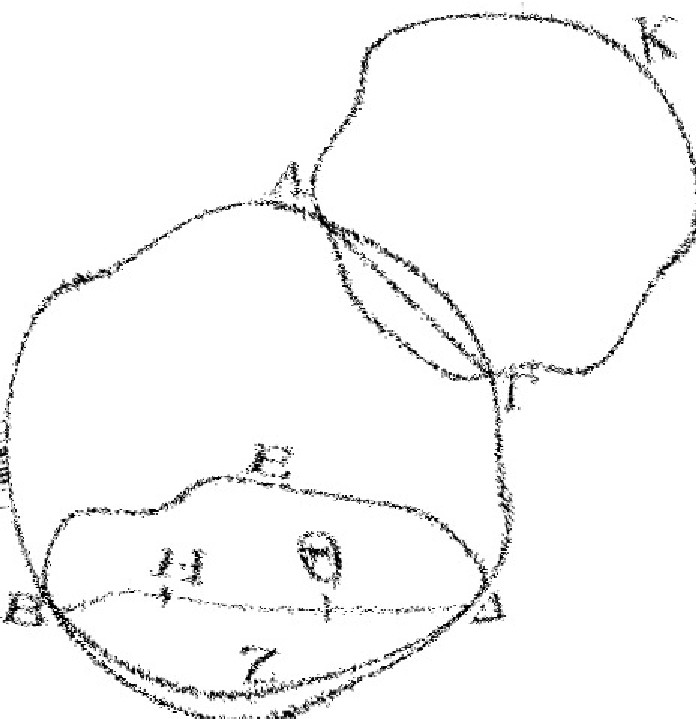
\includegraphics{Book03/front.eps}}
\newpage

%%%%%%%
% Definitions
%%%%%%%
\pdfbookmark[1]{Definitions}{def3}
\pagestyle{fancy}
\cfoot{\gr{\kern -.7pt }}
\lhead{\large\gr{ΣΤΟΙΘΕΙΩΝ \kern -.7pt {3}.}}
\rhead{\large ELEMENTS BOOK 3}
\begin{Parallel}{}{} 
\ParallelLText{
\begin{center}
\large{\gr{<'Οροι}.}
\end{center}\vspace*{-7pt}

\ggn{1}.~\gr{>'Ισοι κύκλοι εἰσίν, <ῶν αἱ διάμετροι >ίσαι εἰσίν,
>ὴ <ῶν αἱ ἐκ τῶν κέντρων >ίσαι εἰσίν.}

\ggn{2}.~\gr{Εὐθεῖα κύκλου ἐφάπτεσθαι λέγεται, <ήτιξ ἁπτομένη τοῦ
κύκλου καὶ ἐκβαλλομένη οὐ τέμνει τὸν κύκλον.}

\ggn{3}.~\gr{Κύκλοι ἐφάπτεσθαι ἀλλήλων λέγονται ο<ίτινεξ ἁπτό\-μενοι ἀλλήλων οὐ τέμνουσιν ἀλλήλουξ.}

\ggn{4}.~\gr{Ἐν κύκλῳ >ίσον ἀπέθειν ἀπὸ τοῦ κέντρου εὐθεῖαι
λέγονται, <όταν αἱ ἀπὸ τοῦ κέντρου ἐπ> α\kern -.7pt  ὐτὰξ κάθετοι ἀγόμεναι
>ίσαι >ῶσιν.}

\ggn{5}.~\gr{Μεῖζον δὲ ἀπέθειν λέγεται, ἐφ> <ὴν ἡ μείζων κάθετοξ πίπτει.}

\ggn{6}.~\gr{Τμ\kern -.7pt  ῆμα κύκλου ἐστὶ τὸ περιεχόμενον σθῆμα ὑπό τε εὐθείαξ καὶ κύκλου περιφερείαξ.}

\ggn{7}.~\gr{Τμ\kern -.7pt  ήματοξ δὲ γωνία ἐστὶν ἡ περιεθομένη ὑπό
τε εὐθείαξ καὶ κύκλου περιφερείαξ.}

\ggn{8}.~\gr{Ἐν τμ\kern -.7pt  ήματι δὲ γωνία ἐστίν, <όταν ἐπὶ τῆξ περιφερείαξ τοῦ τμ\kern -.7pt  ήματοξ ληφθῆ| τι σημεῖον καὶ ἀπ> α\kern -.5pt  ὐτοῦ ἐπὶ τὰ πέρατα
τῆξ εὐθείαξ, <ή ἐστι βάσιξ τοῦ τμ\kern -.3pt  ήματοξ, ἐπιζευθθῶσιν εὐθεῖαι,
ἡ περιεθομένη γωνία ὑπὸ τῶν ἐπιζευθθεισῶν εὐθειῶν.}

\ggn{9}.~\gr{<'Οταν δὲ αἱ περιέθουσαι τὴν γωνίαν εὐθεῖαι ἀπολαμβάνωσί τινα περιφέρειαν, ἐπ> ἐκείνηξ λέγεται βεβηκέναι ἡ γωνία.}

\ggn{10}.~\gr{Τομεὺξ δὲ κύκλου ἐστίν, <όταν πρὸξ τῶ| κέντρῶ| τοῦ
κύκλου συσταθῆ| γωνία, τὸ περιεχόμενον σθῆμα ὑπό τε τῶν τὴν
γωνίαν περιεθουσῶν
εὐθειῶν καὶ τῆξ ἀπολαμβανομένηξ ὑπ> α\kern -.7pt  ὐτῶν περιφερείαξ.}

\ggn{11}.~\gr{<'Ομοία τμ\kern -.7pt  ήματα κύκλων ἐστὶ τὰ δεθόμενα γωνίαξ >ίσαξ, >ή ἐν ο<ῖξ αἱ γωνίαι >ίσαι ἀλλήλαιξ εἰσίν.}}

\ParallelRText{
\begin{center}
{\large Definitions}
\end{center}

1.~Equal circles are (circles) whose diameters are equal,  or whose (distances)
from the centers (to the circumferences) are equal (i.e., whose radii are equal).

2.~A straight-line said to touch a circle  is any (straight-line) which, meeting the circle and being produced, does not cut the circle.

3.~Circles said to touch one another are any (circles) which, meeting one another, do not cut one another.

4.~In a circle, straight-lines are said to be equally far from the center
when the perpendiculars drawn to them from the center are equal.

5.~And (that straight-line) is said to be further (from the center) on
which the greater perpendicular falls (from the center).

6. ~A segment of a circle is the figure contained by a straight-line
and a circumference of a circle.

7.~And the angle of a segment is that contained by a straight-line
and a circumference of a circle.

8.~And the angle in a segment is the
angle contained by the joined straight-lines, when any
point  is taken on the circumference of a segment, 
and straight-lines are joined from it to the ends of the straight-line which is the base of the
segment.

9. ~And when the straight-lines containing an angle cut off some circumference, the angle is said to stand upon that (circumference).

10.~And a sector of a circle is the figure contained by the
straight-lines surrounding an angle, and the circumference cut off by them,
when the angle is constructed at the center of a circle.

11.~Similar segments of circles are those accepting equal angles, or
in which the angles are equal to one another.}
\end{Parallel}

%%%%%%
% Prop 3.1
%%%%%%
\pdfbookmark[1]{Proposition 3.1}{pdf3.1}
\begin{Parallel}{}{} 
\ParallelLText{
\begin{center}
{\large \ggn{1}.}
\end{center}\vspace*{-7pt}

\gr{Τοῦ δοθέντοξ κύκλου τὸ κέντρον εὑρεῖν.}

\gr{>'Εστω ὁ δοθεὶξ κύκλοξ ὁ ΑΒΓ; δεῖ δὴ τοῦ ΑΒΓ κύκλου
τὸ κέντρον εὑρεῖν.}

\gr{Διήθθω τιξ εἰξ α\kern -.7pt  ὐτόν, ὡξ >έτυθεν, εὐθεῖα ἡ ΑΒ, καὶ τετμ\kern -.7pt  ήσθω δίθα
κατὰ τὸ Δ σημεῖον, καὶ ἀπὸ τοῦ Δ τῆ| ΑΒ πρὸξ ὀρθὰξ >ήθθω
ἡ ΔΓ καὶ διήθθω ἐπὶ τὸ Ε, καὶ τετμ\kern -.5pt  ήσθω ἡ ΓΕ δίθα κατὰ τὸ Ζ;
λέγω, <ότι τὸ Ζ κέντρον ἐστὶ τοῦ ΑΒΓ [κύκλου].}

\gr{μ\kern -.7pt  ὴ γάρ, ἀλλ> εἰ δυνατόν, >έστω τὸ Η, καὶ ἐπεζεύθθωσαν αἱ ΗΑ, ΗΔ, ΗΒ. καὶ ἐπεὶ >ίση ἐστὶν ἡ ΑΔ τῆ| ΔΒ, κοινὴ δὲ ἡ ΔΗ, δύο δὴ
αἱ ΑΔ, ΔΗ δύο ταῖξ ΗΔ, ΔΒ >ίσαι εἰσὶν ἑκατέρα ἑκατέρᾳ;
καὶ βάσιξ ἡ ΗΑ βάσει τῆ| ΗΒ ἐστιν >ίση; ἐκ κέντρου γάρ;
γωνία >άρα ἡ ὑπὸ ΑΔΗ γωνίᾳ τῆ| ὑπὸ ΗΔΒ >ίση ἐστίν.
<όταν δὲ εὐθεῖα ἐπ> εὐθεῖαν σταθεῖσα τὰξ ἐφεχῆξ γωνίαξ
>ίσαξ ἀλλήλαιξ ποιῆ|, ὀρθὴ ἑκατέρα τῶν >ίσων γωνιῶν ἐστιν; ὀρθὴ
>άρα ἐστὶν ἡ  ὑπὸ ΗΔΒ. ἐστὶ δὲ καὶ ἡ ὑπὸ ΖΔΒ ὀρθή;
>ίση >άρα ἡ ὑπὸ ΖΔΒ τῆ| ὑπὸ ΗΔΒ, ἡ μείζων τῆ| ἐλάττονι;
<όπερ ἐστὶν ἀδύνατον. οὐκ >άρα τὸ Η κέντρον ἐστὶ τοῦ
ΑΒΓ κύκλου. ὁμοίωξ δὴ δείχομεν, <ότι οὐδ> >άλλο
τι πλὴν τοῦ Ζ.}\\~\\~\\~\\

\epsfysize=2.2in
\centerline{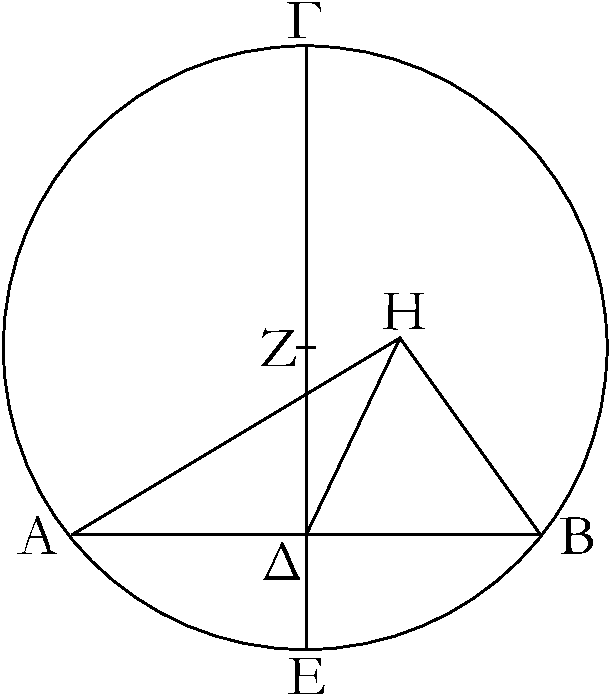
\includegraphics{Book03/fig01g.eps}}

\gr{Τὸ Ζ >άρα σημεῖον κέντρον ἐστὶ τοῦ ΑΒΓ [κύκλου].}

\begin{center}\mbox{}\\
{\large \gr{Πόρισμα}.}
\end{center}\vspace*{-7pt}

\gr{Ἐκ δὴ τούτου φανερόν, <ότι ἒαν ἐν κύκλῳ εὐθεῖά
τιξ εὐθεῖάν τινα δίθα καὶ πρὸξ ὀρθὰξ τέμνῃ, ἐπὶ
τῆξ τεμνούσηξ ἐστὶ τὸ κέντρον τοῦ κύκλου.} --- \gr{<όπερ >έδει
ποιῆσαι.}}

\ParallelRText{
\begin{center}
{\large Proposition 1}
\end{center}

To find the center of a given circle.

Let $ABC$ be the given circle. So it is required to find the center of circle $ABC$.

Let some straight-line $AB$ be drawn through ($ABC$), at random,
and let ($AB$) be cut in half at point $D$ 
[Prop.~1.9]. And let
$DC$ be drawn from $D$, at right-angles to $AB$ [Prop.~1.11].
And let ($CD$) be drawn through to $E$. And let $CE$ be cut in half
at $F$ [Prop.~1.9]. I say that (point) $F$ is the center of the [circle] $ABC$.

For (if) not (then), if possible, let $G$ (be the center of the circle), and
let $GA$, $GD$, and $GB$ be joined. And since $AD$ is equal to $DB$,
and $DG$ (is) common, the two (straight-lines) $AD$, $DG$
are equal to the two (straight-lines) $BD$, $DG$,$^\dag$ respectively. And the
base $GA$ is equal to the base $GB$. For (they are both) radii. Thus, angle
$ADG$ is equal to angle $GDB$ [Prop.~1.8]. And when a straight-line
stood upon (another) straight-line make  adjacent angles (which are)
equal to one another, each of the equal angles is a right-angle [Def.~1.10].
Thus, $GDB$ is a right-angle. And $FDB$ is also a right-angle. Thus,
$FDB$ (is) equal to $GDB$, the greater to the lesser. The very thing
is impossible. Thus, (point) $G$ is not the center of the circle $ABC$. 
So, similarly, we can show that neither is any other (point) except $F$.

\epsfysize=2.2in
\centerline{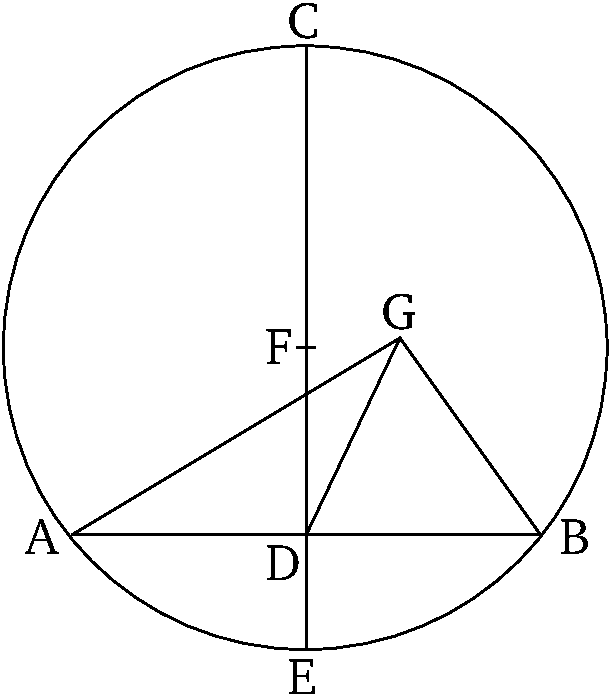
\includegraphics{Book03/fig01e.eps}}

Thus, point $F$ is the center of the [circle] $ABC$.

\begin{center}\mbox{}\\
{\large Corollary}
\end{center}

So, from this, (it is) manifest that if any straight-line in a circle
cuts any (other) straight-line in half, and at right-angles, (then) the center
of the circle is on the former (straight-line). --- (Which is) the very thing it
was required to do.}
\end{Parallel}
{\footnotesize \noindent$^\dag$  The Greek text has ``$GD$, $DB$'', which is obviously a mistake.} 

%%%%%%
% Prop 3.2
%%%%%%
\pdfbookmark[1]{Proposition 3.2}{pdf3.2}
\begin{Parallel}{}{} 
\ParallelLText{
\begin{center}
{\large \ggn{2}.}
\end{center}\vspace*{-7pt}

\gr{Ἐὰν κύκλου ἐπὶ τῆξ περιφερείαξ ληφθῆ| δύο
τυθόντα σημεῖα, ἡ ἐπὶ τὰ σημεῖα ἐπιζευγνυμένη εὐθεῖα
ἐντὸξ πεσεῖται τοῦ κύκλου.}

\gr{>'Εστω κύκλοξ ὁ ΑΒΓ, καὶ ἐπὶ τῆξ περιφερείαξ α\kern -.7pt  ὐτοῦ εἰλήφθω
δύο τυθόντα σημεῖα τὰ Α, Β; λέγω, <ότι ἡ ἀπὸ τοῦ Α ἐπὶ τὸ Β
ἐπιζευγνυμένη εὐθεῖα ἐντὸξ πεσεῖται τοῦ κύκλου.}

\gr{μ\kern -.7pt  ὴ γάρ, ἀλλ> εἰ δυνατόν, πιπτέτω ἐκτὸξ ὡξ ἡ ΑΕΒ, καὶ εἰλήφθω
τὸ κέντρον τοῦ ΑΒΓ κύκλου, καὶ >έστω τὸ Δ, καὶ ἐπεζεύθθωσαν αἱ
ΔΑ, ΔΒ, καὶ διήθθω ἡ ΔΖΕ.}

\gr{Ἐπεὶ ο>ῦν >ίση ἐστὶν ἡ ΔΑ τῆ| ΔΒ, >ίση >άρα
καὶ γωνία ἡ ὑπὸ ΔΑΕ τῆ| ὑπὸ ΔΒΕ; καὶ ἐπεὶ τριγώνου
τοῦ ΔΑΕ μία πλευρὰ προσεκβέβληται ἡ ΑΕΒ, μείζων
>άρα ἡ ὑπὸ ΔΕΒ γωνία τῆξ ὑπὸ ΔΑΕ. >ίση δὲ ἡ ὑπὸ
ΔΑΕ τῆ|  ὑπὸ ΔΒΕ; μείζων >άρα ἡ ὑπὸ ΔΕΒ τῆξ ὑπὸ
ΔΒΕ. ὑπὸ δὲ τὴν μείζονα γωνίαν ἡ μείζων πλευρὰ
ὑποτείνει; μείζων >άρα ἡ ΔΒ τῆξ ΔΕ. >ίση δὲ ἡ ΔΒ
τῆ| ΔΖ. μείζων >άρα ἡ ΔΖ τῆξ ΔΕ ἡ ἐλάττων τῆξ
μείζονοξ; <όπερ ἐστὶν ἀδύνατον. οὐκ >άρα ἡ ἀπὸ
τοῦ Α ἐπὶ τὸ Β ἐπιζευγνυμένη εὐθεῖα ἐκτὸξ
πεσεῖται τοῦ κύκλου. ὁμοίωξ δὴ δείχομεν, <ότι οὐδὲ ἐπ>
α\kern -.7pt  ὐτῆξ τῆξ περιφερείαξ; ἐντὸξ >άρα.}\\~\\~\\

\epsfysize=2.2in
\centerline{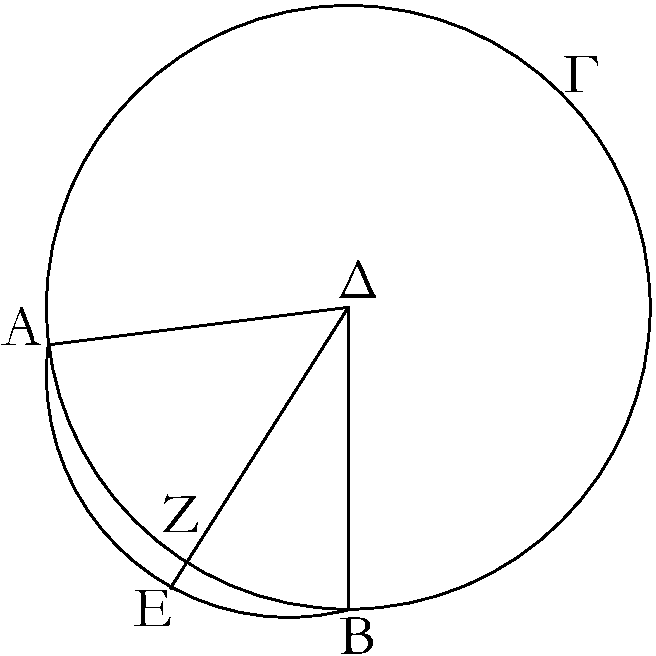
\includegraphics{Book03/fig02g.eps}}

\gr{Ἐὰν >άρα κύκλου ἐπὶ τῆξ περιφερείαξ ληφθῆ| δύο
τυθόντα σημεῖα, ἡ ἐπὶ τὰ σημεῖα ἐπιζευγνυμένη εὐθεῖα
ἐντὸξ πεσεῖται τοῦ κύκλου; <όπερ >έδει δεῖχαι.}}

\ParallelRText{
\begin{center}
{\large Proposition 2}
\end{center}

If two points are taken at random on the circumference of a circle,  (then)
the straight-line joining the points will fall inside the circle.

Let $ABC$ be a circle, and let two points $A$ and $B$ be taken
at random on its circumference. I say that the straight-line joining
$A$ to $B$ will fall inside the circle.

For (if) not (then), if possible, let it fall outside (the circle), like $AEB$ (in the figure). And let the center of the circle $ABC$ be found [Prop.~3.1], and let it be (at point) $D$. And let $DA$ and $DB$ be joined, and let $DFE$ be
drawn through.

Therefore, since $DA$ is equal to $DB$, the angle $DAE$ (is) thus also equal to
$DBE$ [Prop.~1.5]. And since in triangle $DAE$ the one side, $AEB$, has been
produced, angle $DEB$ (is) thus greater than $DAE$ [Prop.~1.16]. And
$DAE$ (is) equal to $DBE$ [Prop.~1.5]. Thus, $DEB$ (is) greater than $DBE$.
And the greater angle is subtended by the greater side [Prop.~1.19].
Thus, $DB$ (is) greater than $DE$. And $DB$ (is) equal to $DF$. Thus,
$DF$ (is) greater than $DE$, the lesser than the greater. The very thing is impossible.
Thus, the straight-line joining $A$ to $B$ will not fall outside the
circle. So, similarly, we can show that neither (will it fall) on the
circumference itself. Thus, (it will fall) inside (the circle).

\epsfysize=2.2in
\centerline{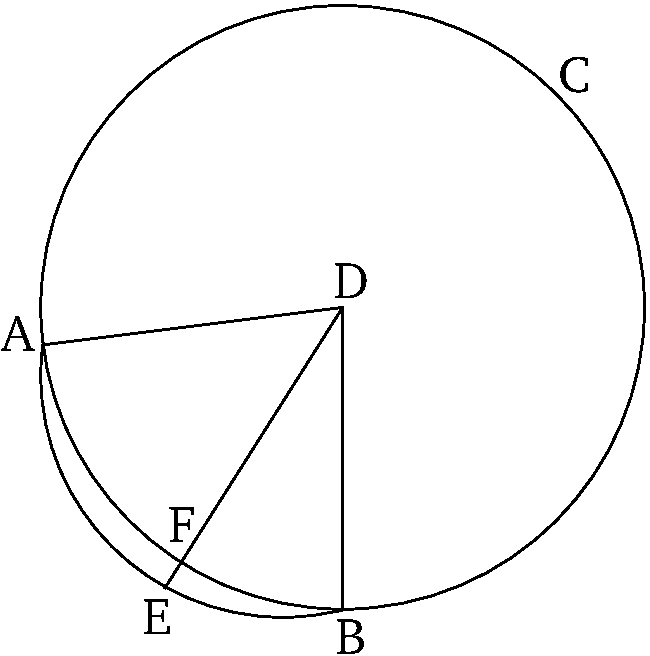
\includegraphics{Book03/fig02e.eps}}

Thus, if two points are taken at random on the circumference of a circle, (then)
the straight-line joining the points will fall inside the circle. (Which is) the
very thing it was required to show.}
\end{Parallel}

%%%%%%
% Prop 3.3
%%%%%%
\pdfbookmark[1]{Proposition 3.3}{pdf3.3}
\begin{Parallel}{}{} 
\ParallelLText{
\begin{center}
{\large \ggn{3}.}
\end{center}\vspace*{-7pt}

\gr{Ἐὰν ἐν κύκλῳ εὐθεῖά τιξ διὰ τοῦ κέντρου εὐθεῖάν τινα μ\kern -.7pt  ὴ διὰ τοῦ κέντρου δίθα τέμνῃ, καὶ πρὸξ ὀρθὰξ α\kern -.7pt  ὐτὴν τέμνει; καὶ ἒαν πρὸξ ὀρθὰξ α\kern -.5pt  ὐτὴν τέμνῃ, καὶ δίθα α\kern -.3pt  ὐτὴν τέμνει.}

\gr{>'Εστω κύκλοξ ὁ ΑΒΓ, καὶ ἐν α\kern -.7pt  ὐτῶ| εὐθεῖά τιξ διὰ τοῦ κέντρου ἡ ΓΔ εὐθεῖάν τινα μ\kern -.7pt  ὴ διὰ τοῦ κέντρου τὴν ΑΒ δίθα τεμνέτω κατὰ τὸ
Ζ σημεῖον; λέγω, <ότι καὶ πρὸξ ὀρθὰξ α\kern -.5pt  ὐτὴν τέμνει.}

\gr{Εἰλήφθω γὰρ τὸ κέντρον τοῦ ΑΒΓ κύκλου, καὶ >έστω τὸ Ε, καὶ ἐπεζεύθθωσαν αἱ ΕΑ, ΕΒ.}

\gr{Καὶ ἐπεὶ >ίση ἐστὶν ἡ ΑΖ τῆ| ΖΒ, κοινὴ δὲ ἡ ΖΕ, δύο δυσὶν >ίσαι [εἰσίν]; καὶ βάσιξ ἡ ΕΑ βάσει τῆ| ΕΒ >ίση; γωνία >άρα ἡ ὑπὸ ΑΖΕ γωνίᾳ τῆ| ὑπὸ ΒΖΕ >ίση ἐστίν. <όταν δὲ εὐθεῖα ἐπ> εὐθεῖαν
σταθεῖσα τὰξ ἐφεχῆξ γωνίαξ >ίσαξ ἀλλήλαιξ ποιῆ|,  ὀρθὴ
ἑκατέρα τῶν >ίσων γωνιῶν ἐστιν; ἑκατέρα >άρα τῶν ὑπὸ ΑΖΕ, ΒΖΕ ὀρθή ἐστιν. ἡ ΓΔ >άρα διὰ τοῦ κέντρου ο>ῦσα τὴν ΑΒ μ\kern -.7pt  ὴ
διὰ τοῦ κέντρου ο>ῦσαν δίθα τέμνουσα καὶ πρὸξ ὀρθὰξ τέμνει.}

\gr{Ἀλλὰ δὴ ἡ ΓΔ τὴν ΑΒ πρὸξ ὀρθὰξ τεμνέτω; λέγω, <ότι καὶ δίθα
α\kern -.7pt  ὐτὴν τέμνει, τουτέστιν, <ότι >ίση ἐστὶν ἡ ΑΖ τῆ| ΖΒ.}

\gr{Τῶν γὰρ α\kern -.7pt  ὐτῶν κατασκευασθέντων, ἐπεὶ >ίση ἐστὶν ἡ ΕΑ τῆ| ΕΒ,
>ίση ἐστὶ καὶ γωνία ἡ ὑπὸ ΕΑΖ τῆ| ὑπὸ ΕΒΖ. ἐστὶ δὲ καὶ
ὀρθὴ ἡ ὑπὸ ΑΖΕ ὀρθῆ| τῆ| ὑπὸ ΒΖΕ >ίση; δύο >άρα τρίγωνά
ἐστι ΕΑΖ, ΕΖΒ τὰξ δύο γωνίαξ δυσὶ γωνίαιξ >ίσαξ >έθοντα καὶ
μίαν πλευρὰν μιᾶ| πλευρᾶ| >ίσην κοινὴν α\kern -.7pt  ὐτῶν τὴν ΕΖ ὑποτείνουσαν ὑπὸ μίαν τῶν >ίσων γωνιῶν; καὶ τὰξ λοιπὰξ >άρα πλευρὰξ ταῖξ
λοιπαῖξ πλευραῖξ >ίσαξ <έχει; >ίση >άρα ἡ ΑΖ τῆ| ΖΒ.}\\~\\~\\~\\

\epsfysize=2.2in
\centerline{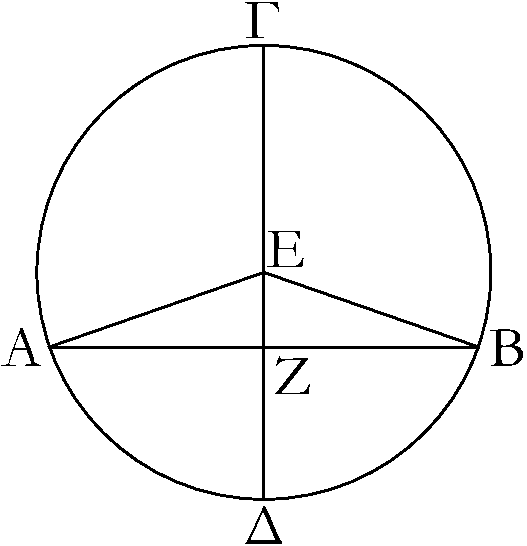
\includegraphics{Book03/fig03g.eps}}

\gr{Ἐὰν >άρα ἐν κύκλῳ εὐθεῖά τιξ διὰ τοῦ κέντρου εὐθεῖάν τινα μ\kern -.7pt  ὴ διὰ τοῦ κέντρου δίθα τέμνῃ, καὶ πρὸξ ὀρθὰξ α\kern -.7pt  ὐτὴν τέμνει; καὶ ἒαν πρὸξ ὀρθὰξ α\kern -.5pt  ὐτὴν τέμνῃ, καὶ δίθα α\kern -.3pt  ὐτὴν τέμνει; <όπερ >έδει δεῖχαι.}}

\ParallelRText{
\begin{center}
{\large Proposition 3}
\end{center}

In a circle, if any straight-line through the center cuts in half any straight-line
not through the center, (then) it also cuts it at right-angles. And (conversely)
if it cuts it at right-angles, (then) it also cuts it in half.

Let $ABC$ be a circle, and, within it, let some straight-line through the center,
$CD$, 
cut in half some straight-line not through the center, $AB$, at the point $F$.
I say that ($CD$) also cuts ($AB$) at right-angles.

For let the center of the circle $ABC$ be found [Prop.~3.1], and let it
be (at point) $E$, and let $EA$ and $EB$ be joined.

And since  $AF$ is equal to $FB$, and $FE$ (is) common, two (sides  of triangle $AFE$) [are] equal to
two (sides of triangle $BFE$). And the base $EA$ (is) equal to the base $EB$. Thus, angle
$AFE$ is equal to angle $BFE$ [Prop.~1.8]. And when a straight-line
stood upon (another) straight-line makes adjacent angles (which are)
equal to one another, each of the equal angles is a right-angle [Def.~1.10].
Thus, $AFE$ and $BFE$ are each right-angles. Thus, the (straight-line) $CD$, which is
through the center
and cuts  in half the (straight-line) $AB$, which is not through the center, also cuts ($AB$) at right-angles.

And so let $CD$ cut $AB$ at right-angles. I say that it also cuts ($AB$) in half.
That is to say, that $AF$ is equal to $FB$.

For, with the same construction, since $EA$ is equal to $EB$, angle $EAF$ is also
equal to $EBF$ [Prop.~1.5]. And the right-angle $AFE$ is also equal to the
right-angle $BFE$. Thus, $EAF$ and $EFB$ are two triangles having two angles
equal to two angles, and one side equal to one side---(namely), their common (side)
$EF$, subtending one of the equal angles. Thus, they will also have the remaining sides equal to the (corresponding) remaining sides [Prop.~1.26]. Thus, $AF$ (is) equal to $FB$.

\epsfysize=2.2in
\centerline{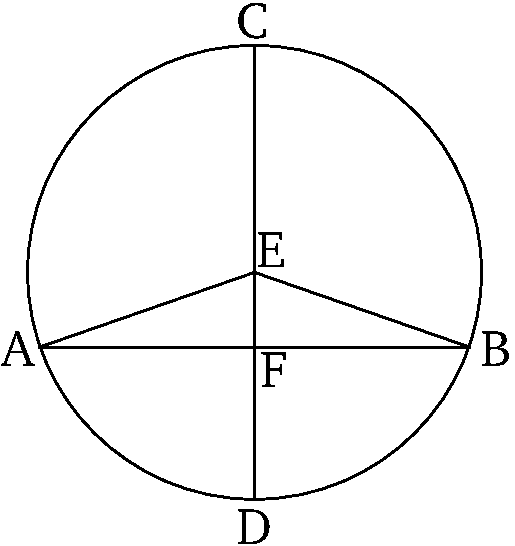
\includegraphics{Book03/fig03e.eps}}

Thus, in a circle, if any straight-line through the center cuts in half any straight-line
not through the center, (then) it also cuts it at right-angles. And (conversely)
if it cuts it at right-angles, (then) it also cuts it in half. (Which is) the very thing
it was required to show.}
\end{Parallel}

%%%%%%
% Prop 3.4
%%%%%%
\pdfbookmark[1]{Proposition 3.4}{pdf3.4}
\begin{Parallel}{}{} 
\ParallelLText{
\begin{center}
{\large \ggn{4}.}
\end{center}\vspace*{-7pt}

\gr{Ἐὰν ἐν κύκλῳ δύο εὐθεῖαι τέμνωσιν ἀλλήλαξ μ\kern -.7pt  ὴ δὶα τοῦ
κέντρου ο>ῦσαι, οὐ τέμνουσιν ἀλλήλαξ δίθα.}\\

\epsfysize=2in
\centerline{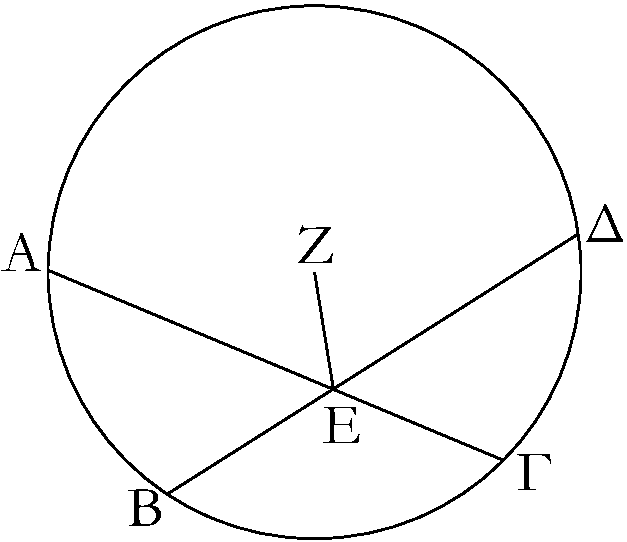
\includegraphics{Book03/fig04g.eps}}

\gr{>'Εστω κύκλοξ ὁ ΑΒΓΔ, καὶ ἐν α\kern -.7pt  ὐτῶ| δύο εὐθεῖαι αἱ ΑΓ,
ΒΔ τεμνέτωσαν ἀλλήλαξ κατὰ τὸ Ε μ\kern -.7pt  ὴ διὰ τοῦ κέντρου ο>ῦσαι;
λέγω, <ότι οὐ τέμνουσιν ἀλλήλαξ δίθα.}

\gr{Εἰ γὰρ δυνατόν, τεμνέτωσαν ἀλλήλαξ δίθα <ώστε >ίσην ε>ῖναι
τὴν μὲν ΑΕ τῆ| ΕΓ, τὴν δὲ ΒΕ τῆ| ΕΔ; καὶ εἰλήφθω τὸ κέντρον
τοῦ ΑΒΓΔ κύκλου, καὶ >έστω τὸ Ζ, καὶ ἐπεζεύθθω ἡ ΖΕ.}

\gr{Ἐπεὶ ο>ῦν εὐθεῖά τιξ διὰ τοῦ κέντρου ἡ ΖΕ εὐθεῖάν τινα
μ\kern -.7pt  ὴ διὰ τοῦ κέντρου τὴν ΑΓ δίθα τέμνει, καὶ πρὸξ ὀρθὰξ α\kern -.7pt  ὐτὴν τέμνει; ὀρθὴ >άρα ἐστὶν ἡ ὑπὸ ΖΕΑ; πάλιν, ἐπεὶ εὐθεῖά τιξ ἡ ΖΕ εὐθεῖάν τινα τὴν ΒΔ δίθα τέμνει, καὶ πρὸξ ὀρθὰξ α\kern -.5pt  ὐτὴν τέμνει;
ὀρθὴ >άρα ἡ ὑπὸ ΖΕΒ. ἐδείθθη δὲ καὶ ἡ ὑπὸ ΖΕΑ ὀρθή; >ίση >άρα ἡ ὑπὸ ΖΕΑ τῆ| ὑπὸ ΖΕΒ ἡ ἐλάττων τῆ| μείζονι;
<όπερ ἐστὶν ἀδύνατον. οὐκ >άρα αἱ ΑΓ, ΒΔ τέμνουσιν ἀλλήλαξ δίθα.}

\gr{Ἐὰν >άρα ἐν κύκλῳ δύο εὐθεῖαι τέμνωσιν ἀλλήλαξ μ\kern -.7pt  ὴ δὶα τοῦ
κέντρου ο>ῦσαι, οὐ τέμνουσιν ἀλλήλαξ δίθα; <όπερ >έδει δεῖχαι.}}

\ParallelRText{
\begin{center}
{\large Proposition 4}
\end{center}

In a circle, if two straight-lines, which are not through the center, cut
one another, (then) they do not cut one another in half.

\epsfysize=2in
\centerline{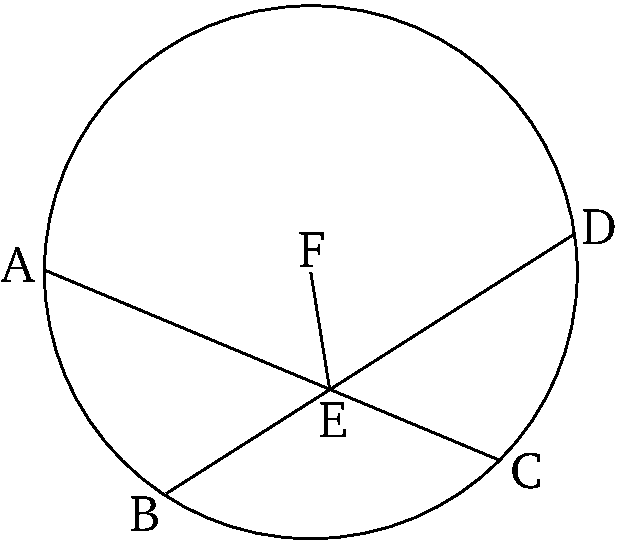
\includegraphics{Book03/fig04e.eps}}

Let $ABCD$ be a circle, and within it, let two straight-lines, $AC$ and
$BD$, which are not through the center, cut one another at  (point) $E$. I say that they
do not cut one another in half.

For, if possible, let them cut one another in half, such that $AE$ is equal to $EC$, and
$BE$ to $ED$. And let the center of the circle $ABCD$ be found [Prop.~3.1], and let it be (at point) $F$, and let $FE$ be joined.

Therefore, since some straight-line through the center, $FE$, cuts in half
some straight-line not through the center, $AC$, it also cuts it at right-angles
[Prop.~3.3]. Thus, $FEA$ is a right-angle. Again, since some straight-line
$FE$ cuts in half some straight-line $BD$, it also cuts it at right-angles [Prop.~3.3]. Thus, $FEB$ (is) a right-angle. But $FEA$ was also shown (to be) a right-angle. Thus, $FEA$ (is) equal to $FEB$, the lesser to the greater.
The very thing is impossible. Thus, $AC$ and $BD$ do not cut one another in half.

Thus, in a circle, if two straight-lines, which are not through the center, cut
one another, (then) they do not cut one another in half. (Which is) the very
thing it was required to show.}
\end{Parallel}

%%%%%%
% Prop 3.5
%%%%%%
\pdfbookmark[1]{Proposition 3.5}{pdf3.5}
\begin{Parallel}{}{} 
\ParallelLText{
\begin{center}
{\large \ggn{5}.}
\end{center}\vspace*{-7pt}

\gr{Ἐὰν δύο κύκλοι τέμνωσιν ἀλλήλουξ, οὐκ >έσται α\kern -.7pt  ὐτῶν τὸ α\kern -.7pt  ὐτὸ
κέντρον.}

\epsfysize=2in
\centerline{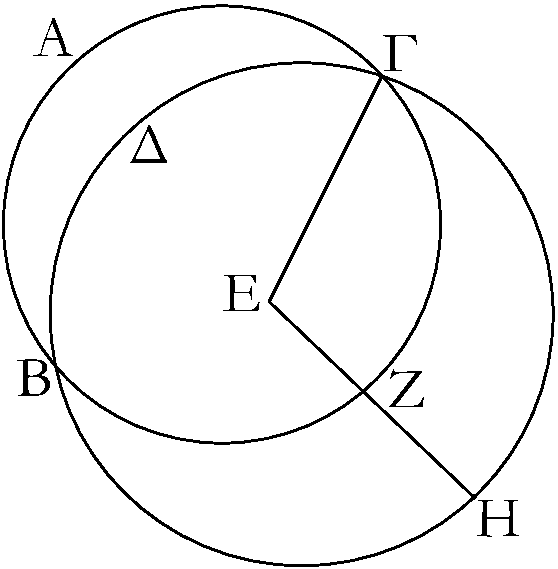
\includegraphics{Book03/fig05g.eps}}

\gr{Δύο γὰρ κύκλοι οἱ ΑΒΓ, ΓΔΗ τεμνέτωσαν ἀλλήλουξ κατὰ τὰ Β, Γ σημεῖα. λέγω, <ότι οὐκ >έσται α\kern -.7pt  ὐτῶν τὸ α\kern -.7pt  ὐτὸ κέντρον.}

\gr{Εἰ γὰρ δυνατόν, >έστω τὸ Ε, καὶ ἐπεζεύθθω ἡ ΕΓ, καὶ διήθθω
ἡ ΕΖΗ, ὡξ >έτυθεν. καὶ ἐπεὶ τὸ Ε σημεῖον κέντρον ἐστὶ τοῦ ΑΒΓ κύκλου, <ίση ἐστὶν ἡ ΕΓ τῆ| ΕΖ. πάλιν, ἐπεὶ τὸ Ε σημεῖον κέντρον ἐστὶ τοῦ ΓΔΗ κύκλου, >ίση ἐστὶν ἡ ΕΓ τῆ| ΕΗ; ἐδείθθη
δὲ ἡ ΕΓ καὶ τῆ| ΕΖ >ίση; καὶ ἡ ΕΖ >άρα τῆ| ΕΗ ἐστιν >ίση ἡ
ἐλάσσων τῆ| μείζονι; <όπερ ἐστὶν ἀδύνατον.  οὐκ >άρα τὸ Ε
σημεῖον κέντρον ἐστὶ τῶν ΑΒΓ, ΓΔΗ κύκλων.}

\gr{Ἐὰν >άρα δύο κύκλοι τέμνωσιν ἀλλήλουξ, οὐκ >έστιν α\kern -.7pt  ὐτῶν τὸ
α\kern -.7pt  ὐτὸ κέντρον; <όπερ >έδει δεῖχαι.}}

\ParallelRText{
\begin{center}
{\large Proposition 5}
\end{center}

If two circles cut one another,  (then) they will not have the same center.

\epsfysize=2in
\centerline{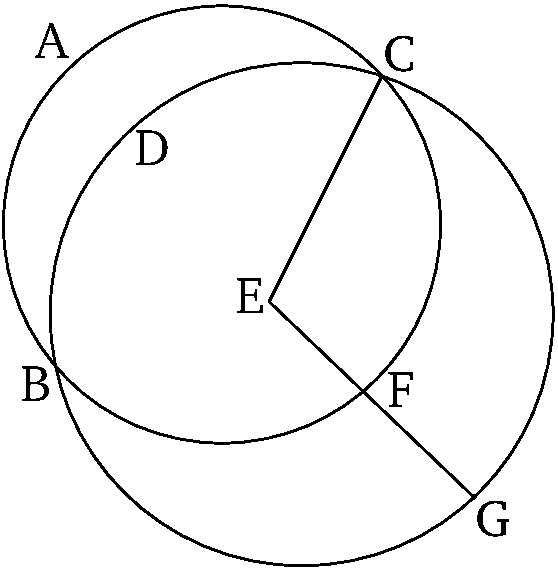
\includegraphics{Book03/fig05e.eps}}

For let the two circles $ABC$ and $CDG$ cut one another at  points $B$ and $C$.
I say that they will not have the same center.

For, if possible, let $E$ be (the common center), and let $EC$ be joined,
and let $EFG$ be drawn through (the two circles), at random. And since point $E$
is the center of the circle $ABC$, $EC$ is equal to $EF$. Again, since point $E$ is
the center of the circle $CDG$, $EC$ is equal to $EG$. But $EC$  was also shown (to be) equal to $EF$. Thus, $EF$ is also equal to $EG$, the lesser to the
greater. The very thing is impossible. Thus, point $E$ is not the (common)
center of the circles $ABC$ and $CDG$.

Thus, if two circles cut one another, (then) they will not have the same
center. (Which is) the very thing it was required to show.}
\end{Parallel}

%%%%%%
% Prop 3.6
%%%%%%
\pdfbookmark[1]{Proposition 3.6}{pdf3.6}
\begin{Parallel}{}{} 
\ParallelLText{
\begin{center}
{\large \ggn{6}.}
\end{center}\vspace*{-7pt}

\gr{Ἐὰν δύο κύκλοι ἐφάπτωνται ἀλλήλων, οὐκ >έσται α\kern -.7pt  ὐτῶν τὸ α\kern -.7pt  ὐτὸ κέντρον.}

\gr{Δύο γὰρ κύκλοι οἱ ΑΒΓ, ΓΔΕ ἐφαπτέσθωσαν ἀλλήλων κατὰ τὸ Γ
σημεῖον; λέγω, <ότι οὐκ >έσται α\kern -.7pt  ὐτῶν τὸ α\kern -.7pt  ὐτὸ κέντρον.}

\gr{Εἰ γὰρ δυνατόν, >έστω τὸ Ζ, καὶ ἐπεζεύθθω ἡ ΖΓ, καὶ διήθθω, ὡξ >έτυθεν, ἡ ΖΕΒ.}

\gr{Ἐπεὶ ο~ὐν τὸ Ζ σημεῖον κέντρον ἐστὶ τοῦ ΑΒΓ κύκλου, >ίση
ἐστὶν ἡ ΖΓ τῆ| ΖΒ. πάλιν, ἐπεὶ τὸ Ζ σημεῖον κέντρον ἐστὶ τοῦ ΓΔΕ κύκλου, >ίση ἐστὶν ἡ ΖΓ τῆ| ΖΕ. ἐδείθθη δὲ ἡ ΖΓ τῆ| ΖΒ
>ίση; καὶ ἡ ΖΕ >άρα τῆ| ΖΒ ἐστιν >ίση, ἡ ἐλάττων τῆ| μείζονι;
<όπερ ἐστὶν ἀδύνατον. οὐκ >άρα τὸ Ζ σημεῖον κέντρον ἐστὶ
τῶν ΑΒΓ, ΓΔΕ κύκλων.}

\epsfysize=2.2in
\centerline{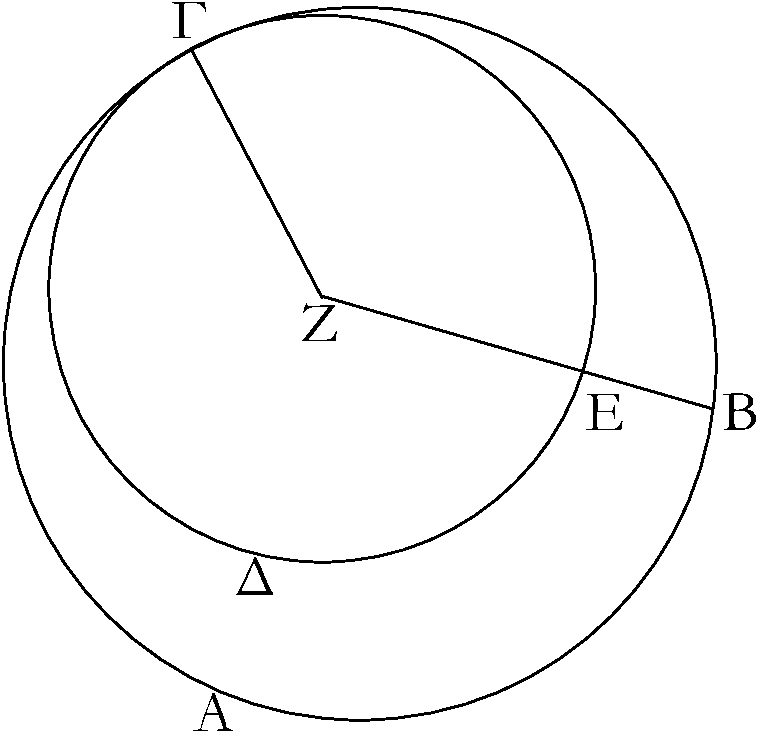
\includegraphics{Book03/fig06g.eps}}

\gr{Ἐὰν >άρα δύο κύκλοι ἐφάπτωνται ἀλλήλων, οὐκ >έσται α\kern -.7pt  ὐτῶν τὸ α\kern -.7pt  ὐτὸ κέντρον; <όπερ >έδει δεῖχαι.}}

\ParallelRText{
\begin{center}
{\large Proposition 6}
\end{center}

If  two circles touch one another, (then) they  will not have the same center.

For let the two circles $ABC$ and $CDE$ touch one another at point $C$. I say that
they will not have the same center.

For, if possible, let $F$ be (the common center), and let $FC$ be
joined, and let $FEB$ be drawn through (the two circles), at random.

Therefore, since point $F$ is the center of the circle $ABC$, $FC$ is equal to
$FB$. Again, since point $F$ is the center of the circle $CDE$, $FC$ is
equal to $FE$. But $FC$ was shown (to be) equal to $FB$. Thus, $FE$ is
also equal to $FB$, the lesser to the greater. The very thing is impossible.
Thus, point $F$ is not the (common) center of the circles
$ABC$ and $CDE$.

\epsfysize=2.2in
\centerline{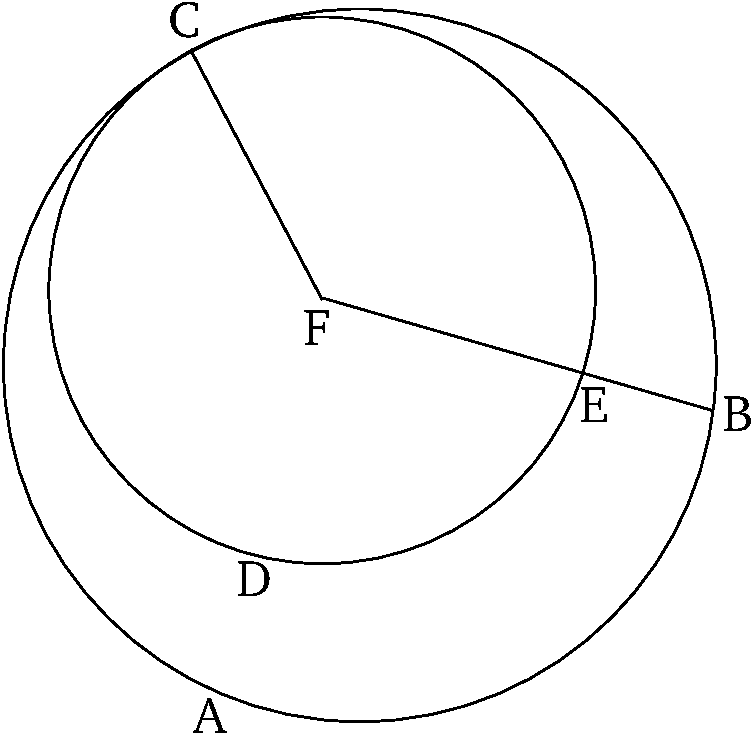
\includegraphics{Book03/fig06e.eps}}

Thus, if two circles touch one another, (then) they  will not have the same center. (Which is) the very thing it was required to show.}
\end{Parallel}

%%%%%%
% Prop 3.7
%%%%%%
\pdfbookmark[1]{Proposition 3.7}{pdf3.7}
\begin{Parallel}{}{} 
\ParallelLText{
\begin{center}
{\large \ggn{7}.}
\end{center}\vspace*{-7pt}

\gr{Ἐὰν κύκλου ἐπὶ τῆξ διαμέτρου ληφθῆ| τι σημεῖον, <ὸ μ\kern -.7pt  ή ἐστι κέντρον τοῦ κύκλου, ἀπὸ δὲ τοῦ σημείου πρὸξ τὸν κύκλον προσπίπτωσιν εὐθεῖαί τινεξ, μεγίστη μὲν >έσται, ἐφ> <ῆξ
τὸ κέντρον, ἐλαθίστη δὲ ἡ λοιπή, τῶν δὲ >άλλων ἀεὶ ἡ
>έγγιον τῆξ δὶα τοῦ κέντρου τῆξ ἀπώτερον μείζων ἐστίν, δύο
δὲ μόνον >ίσαι ἀπὸ τοῦ σημείου προσπεσοῦνται πρὸξ τὸν
κύκλον ἐφ> ἑκάτερα τῆξ ἐλαθίστηξ.}

\gr{>'Εστω κύκλοξ ὁ ΑΒΓΔ, διάμετροξ δὲ α\kern -.7pt  ὐτοῦ >έστω ἡ ΑΔ, καὶ ἐπὶ
τῆξ ΑΔ εἰλήφθω τι σημεῖον τὸ Ζ, <ὸ μ\kern -.7pt  ή ἐστι κέντρον τοῦ κύκλου, κέντρον δὲ τοῦ κύκλου >έστω τὸ Ε, καὶ ἀπὸ τοῦ Ζ πρὸξ τὸν ΑΒΓΔ κύκλον προσπιπτέτωσαν εὐθεῖαί τινεξ αἱ ΖΒ, ΖΓ, ΖΗ; λέγω, <ότι
μεγίστη μέν ἐστιν ἡ ΖΑ, ἐλαθίστη δὲ ἡ ΖΔ, τῶν δὲ >άλλων ἡ μὲν
ΖΒ τῆξ ΖΓ μείζων, ἡ δὲ ΖΓ τῆξ ΖΗ.}

\gr{Ἐπεζεύθθωσαν γὰρ αἱ ΒΕ, ΓΕ, ΗΕ. καὶ ἐπεὶ παντὸξ τριγώνου αἱ δύο πλευραὶ τῆξ λοιπῆξ μείζονέξ εἰσιν, αἱ >άρα ΕΒ, ΕΖ τῆξ ΒΖ μείζονέξ
εἰσιν. >ίση δὲ ἡ ΑΕ τῆ| ΒΕ [αἱ >άρα ΒΕ, ΕΖ >ίσαι εἰσὶ τῆ| ΑΖ];
μείζων >άρα ἡ ΑΖ τῆξ ΒΖ. πάλιν, ἐπεὶ >ίση ἐστὶν ἡ ΒΕ τῆ| ΓΕ,
κοινὴ δὲ ἡ ΖΕ, δύο δὴ αἱ ΒΕ, ΕΖ δυσὶ ταῖξ ΓΕ, ΕΖ >ίσαι εἰσίν.
ἀλλὰ καὶ γωνία ἡ ὑπὸ ΒΕΖ γωνίαξ τῆξ ὑπὸ ΓΕΖ μείζων; βάσιξ
>άρα ἡ ΒΖ βάσεωξ τῆξ ΓΖ μείζων ἐστίν. διὰ τὰ α\kern -.7pt  ὐτὰ δὴ καὶ
ἡ ΓΖ τῆξ ΖΗ μείζων ἐστίν.}

\gr{Πάλιν, ἐπεὶ αἱ ΗΖ, ΖΕ τῆξ ΕΗ μείζονέξ εἰσιν, >ίση δὲ ἡ ΕΗ
τῆ| ΕΔ, αἱ >άρα ΗΖ, ΖΕ τῆξ ΕΔ μείζονέξ εἰσιν. κοινὴ ἀφῃρήσθω ἡ ΕΖ; λοιπὴ >άρα ἡ ΗΖ λοιπῆξ τῆξ ΖΔ μείζων ἐστίν. μεγίστη μὲν >άρα ἡ ΖΑ, ἐλαθίστη δὲ ἡ ΖΔ, μείζων δὲ ἡ μὲν ΖΒ τῆξ ΖΓ, ἡ
δὲ ΖΓ τῆξ ΖΗ.}\\~\\~\\~\\~\\~\\~\\

\epsfysize=2.5in
\centerline{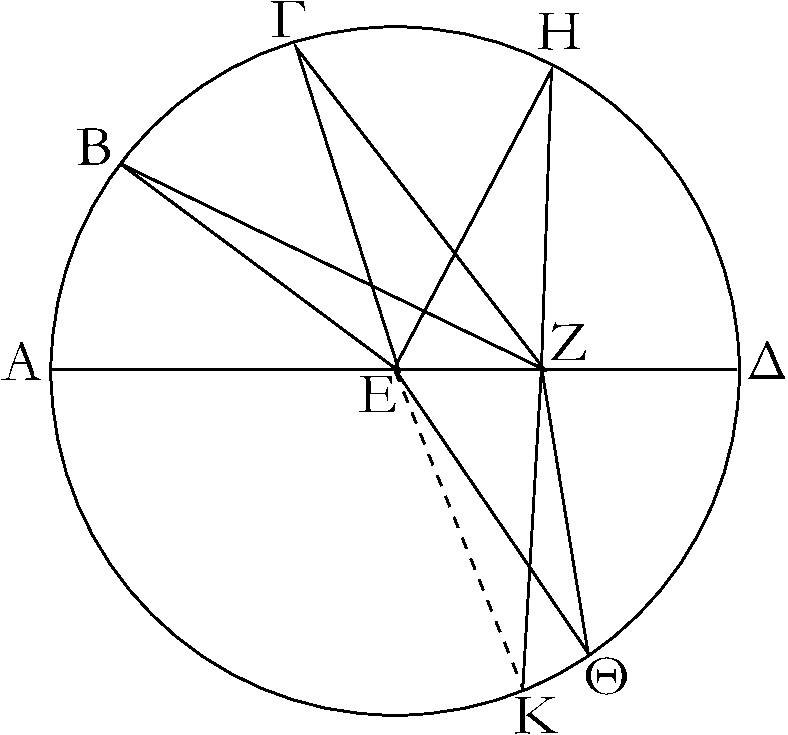
\includegraphics{Book03/fig07g.eps}}

\gr{Λέγω, <ότι καὶ ἀπὸ τοῦ Ζ σημείου δύο μόνον >ίσαι προσπεσοῦνται πρὸξ τὸν ΑΒΓΔ κύκλον ἐφ> ἑκάτερα τῆξ ΖΔ ἐλαθίστηξ. συνεστάτω γὰρ πρὸξ τῆ| ΕΖ εὐθείᾳ καὶ τῶ| πρὸξ α\kern -.7pt  ὐτῆ| σημείῳ τῶ| Ε τῆ|
ὑπὸ ΗΕΖ γωνίᾳ >ίση ἡ ὑπὸ ΖΕJ, καὶ ἐπεζεύθθω ἡ ΖJ. ἐπεὶ ο>ῦν >ίση ἐστὶν ἡ ΗΕ τῆ| ΕJ, κοινὴ δὲ ἡ ΕΖ, δύο
δὴ αἱ ΗΕ, ΕΖ δυσὶ ταῖξ JΕ, ΕΖ >ίσαι εἰσίν; καὶ γωνία ἡ ὑπὸ ΗΕΖ
γωνίᾳ τῆ| ὑπὸ JΕΖ >ίση; βάσιξ >άρα ἡ ΖΗ βάσει τῆ| ΖJ >ίση
ἐστίν. λέγω δή, <ότι τῆ| ΖΗ >άλλη >ίση οὐ προσπεσεῖται πρὸξ τὸν
κύκλον ἀπὸ τοῦ Ζ σημείου. εἰ γὰρ δυνατόν, προσπιπτέτω ἡ ΖΚ.
καὶ ἐπεὶ ἡ ΖΚ τῆ| ΖΗ >ίση ἐστίν, ἀλλὰ ἡ ΖJ τῆ| ΖΗ
[>ίση ἐστίν], καὶ  ἡ  ΖΚ
>άρα τῆ| ΖJ ἐστιν >ίση, ἡ >έγγιον
τῆξ διὰ τοῦ κέντρου τῆ| ἀπώτερον >ίση; <όπερ ἀδύνατον.
οὐκ >άρα ἀπὸ τοῦ Ζ σημείου ἑτέρα τιξ προσπεσεῖται πρὸξ τὸν
κύκλον >ίση τῆ| ΗΖ; μία >άρα μόνη.}

\gr{Ἐὰν >άρα κύκλου ἐπὶ τῆξ διαμέτρου ληφθῆ| τι σημεῖον, <ὸ μ\kern -.7pt  ή ἐστι κέντρον τοῦ κύκλου, ἀπὸ δὲ τοῦ σημείου πρὸξ τὸν κύκλον προσπίπτωσιν εὐθεῖαί τινεξ, μεγίστη μὲν >έσται, ἐφ> <ῆξ
τὸ κέντρον, ἐλαθίστη δὲ ἡ λοιπή, τῶν δὲ >άλλων ἀεὶ ἡ
>έγγιον τῆξ δὶα τοῦ κέντρου τῆξ ἀπώτερον μείζων ἐστίν, δύο
δὲ μόνον >ίσαι ἀπὸ τοῦ α\kern -.7pt  ὐτοῦ σημείου προσπεσοῦνται πρὸξ τὸν
κύκλον ἐφ> ἑκάτερα τῆξ ἐλαθίστηξ; <όπερ >έδει δεῖχαι.}}

\ParallelRText{
\begin{center}
{\large Proposition 7}
\end{center}

If some point, which is not the
center of the circle, is taken on the diameter of a circle,
and some straight-lines radiate from the point towards
the (circumference of the) circle, (then) the greatest (straight-line) will be that on which
the center (lies), and the least the remainder (of the same diameter). And
for the others, a (straight-line) nearer$^\dag$ to the (straight-line) through the center is always
greater than a (straight-line) further away. And only two equal (straight-lines)
will radiate from the point towards the (circumference of the) circle, (one)
on each (side) of the least (straight-line).

Let $ABCD$ be a circle, and let $AD$ be its diameter, and
let some point $F$, which is not the center of the circle, be taken on $AD$.
Let $E$ be the center of the circle. And let some straight-lines, $FB$, $FC$,
and $FG$, radiate from $F$ towards (the circumference of) circle $ABCD$.
I say that $FA$ is the greatest (straight-line), $FD$ the least, and of the others, $FB$ (is)
greater than $FC$, and $FC$ than $FG$.

For let $BE$, $CE$, and $GE$ be joined. And since for every triangle
(any) two sides are greater than the remaining (side) [Prop.~1.20],
$EB$ and $EF$ is thus greater than $BF$. And $AE$ (is) equal to $BE$ [thus,
$BE$ and $EF$ is equal to $AF$]. Thus, $AF$ (is) greater than $BF$. Again,
since $BE$ is equal to $CE$, and $FE$ (is) common, the two (straight-lines)
$BE$, $EF$ are equal to the two (straight-lines) $CE$, $EF$ (respectively). But, angle $BEF$ (is)
also greater than angle $CEF$.$^\ddag$ Thus, the base $BF$ is greater than the base $CF$.
Thus, the base $BF$ is greater than the base $CF$ [Prop.~1.24]. So, for the same (reasons), $CF$ is also greater than $FG$.

Again, since $GF$ and $FE$ are greater than $EG$ [Prop.~1.20], and $EG$
(is) equal to $ED$, $GF$ and $FE$ are thus greater than $ED$. Let $EF$ be
taken from both. Thus, the remainder $GF$ is greater than the remainder $FD$.
Thus, $FA$ (is) the greatest  (straight-line), $FD$ the least, and $FB$ (is) greater than $FC$, and $FC$ than $FG$.

\epsfysize=2.5in
\centerline{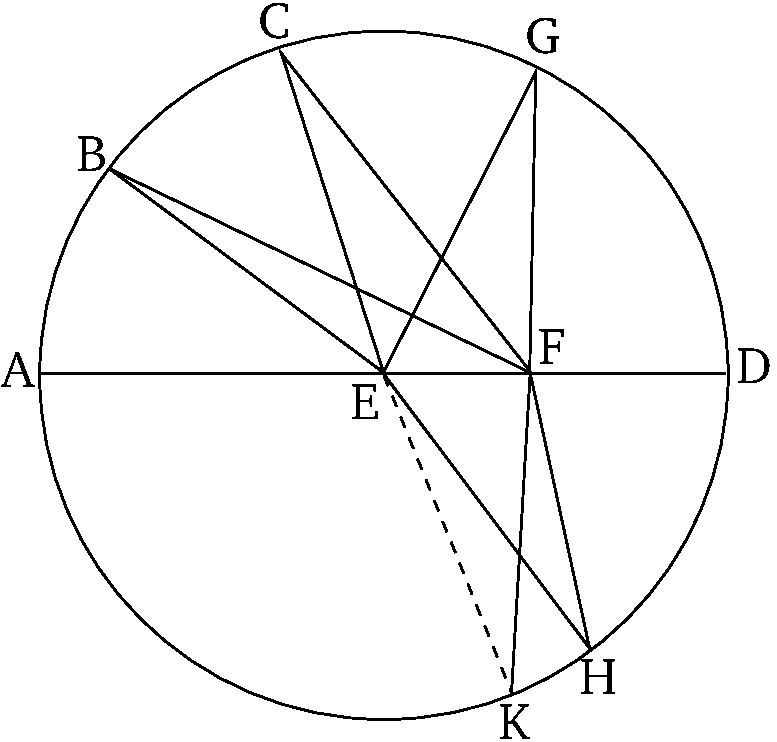
\includegraphics{Book03/fig07e.eps}}

I also say that from point $F$ only two equal (straight-lines) will radiate
towards (the circumference of) circle $ABCD$, (one) on each (side) of the
least (straight-line) $FD$. For let the (angle) $FEH$, equal to angle $GEF$, be constructed on the straight-line $EF$, at the point $E$ on it [Prop.~1.23], and
let $FH$ be joined. Therefore, since $GE$ is equal to $EH$, and $EF$ (is) common, the two (straight-lines) $GE$, $EF$ are equal to the two (straight-lines)
$HE$, $EF$ (respectively). And angle $GEF$ (is) equal to angle $HEF$. Thus, the base $FG$ is
equal to the base $FH$ [Prop.~1.4]. So I say that another (straight-line)
equal to $FG$
will not radiate towards (the circumference of)
the circle from point $F$. For, if possible, let $FK$ (so) radiate. And since
$FK$ is equal to $FG$, but $FH$ [is equal] to $FG$, $FK$ is thus also equal to
$FH$, the nearer to the (straight-line) through the center equal to the
further away. The very thing (is) impossible. Thus, another (straight-line)
equal to $GF$ will not radiate from the point $F$ towards (the circumference of) the circle.
Thus, (there is) only one (such straight-line).

Thus, if some point, which is not the
center of the circle, is taken on the diameter of a circle,
and some straight-lines radiate from the point towards
the (circumference of the) circle, (then) the greatest (straight-line) will be that on which
the center (lies), and the least the remainder (of the same diameter). And
for the others, a (straight-line) nearer to the (straight-line) through the center is always
greater than a (straight-line) further away. And only two equal (straight-lines)
will radiate from the same point towards the (circumference of the) circle,  (one)
on each (side) of the least (straight-line). (Which is) the very thing it was required to show.}
\end{Parallel}
{\footnotesize \noindent$^\dag$ Presumably, in an angular sense.\\
$^\ddag$ This is not proved, except by reference to the figure.}

%%%%%%
% Prop 3.8
%%%%%%
\pdfbookmark[1]{Proposition 3.8}{pdf3.8}
\begin{Parallel}{}{} 
\ParallelLText{
\begin{center}
{\large \ggn{8}.}
\end{center}\vspace*{-7pt}

\gr{Ἐὰν κύκλου ληφθῆ| τι σημεῖον ἐκτόξ, ἀπὸ δὲ τοῦ σημείου πρὸξ
τὸν κύκλον διαθθῶσιν εὐθεῖαί τινεξ, <ῶν μία μὲν διὰ τοῦ κέντρου,
αἱ δὲ λοιπαί, ὡξ >έτυθεν, τῶν μὲν πρὸξ τὴν κοίλην περιφέρειαν προσπιπτουσῶν εὐθειῶν μεγίστη μέν ἐστιν ἡ διὰ τοῦ κέντρου, τῶν δὲ >άλλων ἀεὶ ἡ >έγγιον τῆξ διὰ τοῦ κέντρου τῆξ ἀπώτερον μείζων ἐστίν, τῶν δὲ πρὸξ τὴν κυρτὴν περιφέρειαν προσπιπτουσῶν εὐθειῶν
ἐλαθίστη μέν ἐστιν ἡ μεταχὺ τοῦ τε σημείου καὶ τῆξ διαμέτρου, τῶν δὲ >άλλων ἀεὶ ἡ >έγγιον τῆξ ἐλαθίστηξ τῆξ ἀπώτερόν ἐστιν
ἐλάττων, δύο δὲ μόνον >ίσαι ἀπὸ τοῦ σημείου προσπεσοῦνται
πρὸξ τὸν κύκλον ἐφ> ἑκάτερα τῆξ ἐλαθίστηξ.}

\gr{>'Εστω κύκλοξ ὁ ΑΒΓ, καὶ τοῦ ΑΒΓ εἰλήφθω τι σημεῖον ἐκτὸξ τὸ Δ,
καὶ ἀπ> α\kern -.7pt  ὐτοῦ διήθθωσαν εὐθεῖαί τινεξ αἱ ΔΑ, ΔΕ, ΔΖ, ΔΓ,
>έστω δὲ ἡ ΔΑ διὰ τοῦ κέντρου. λέγω, <ότι τῶν μὲν πρὸξ
τὴν ΑΕΖΓ κοίλην περιφέρειαν προσπιπτουσῶν εὐθειῶν μεγίστη
μέν ἐστιν ἡ διὰ τοῦ κέντρου ἡ ΔΑ, μείζων δὲ ἡ μὲν ΔΕ τῆξ ΔΖ ἡ δὲ ΔΖ τῆξ ΔΓ, τῶν δὲ πρὸξ τὴν JΛΚΗ κυρτὴν περιφέρειαν προσπιπτουσῶν εὐθειῶν ἐλαθίστη μέν ἐστιν ἡ ΔΗ ἡ
μεταχὺ τοῦ σημείου καὶ τῆξ διαμέτρου τῆξ ΑΗ, ἀεὶ δὲ ἡ
>έγγιον τῆξ ΔΗ ἐλαθίστηξ ἐλάττων ἐστὶ τῆξ ἀπώτερον, ἡ μὲν
ΔΚ τῆξ ΔΛ, ἡ δὲ ΔΛ τῆξ ΔJ.}

\gr{Εἰλήφθω γὰρ τὸ κέντρον τοῦ ΑΒΓ κύκλου καὶ >έστω τὸ Μ; καὶ
ἐπεζεύθθωσαν αἱ ΜΕ, ΜΖ, ΜΓ, ΜΚ, ΜΛ, ΜJ.}

\gr{Καὶ ἐπεὶ >ίση ἐστὶν ἡ ΑΜ τῆ| ΕΜ, κοινὴ προσκείσθω ἡ ΜΔ;
ἡ >άρα ΑΔ >ίση ἐστὶ ταῖξ ΕΜ, ΜΔ. ἀλλ> αἱ ΕΜ, ΜΔ τῆξ ΕΔ μείζονέξ εἰσιν; καὶ ἡ ΑΔ >άρα τῆξ ΕΔ μείζων ἐστίν. πάλιν, ἐπεὶ
>ίση ἐστὶν ἡ ΜΕ τῆ| ΜΖ, κοινὴ δὲ ἡ ΜΔ, αἱ ΕΜ, ΜΔ >άρα
ταῖξ ΖΜ, ΜΔ >ίσαι εἰσίν; καὶ γωνία ἡ ὑπὸ ΕΜΔ γωνίαξ τῆξ ὑπὸ ΖΜΔ μείζων ἐστίν. βάσιξ >άρα ἡ ΕΔ βάσεωξ τῆξ ΖΔ μείζων ἐστίν.
ὁμοίωξ δὴ δείχομεν, <ότι καὶ ἡ ΖΔ τῆξ
ΓΔ μείζων ἐστίν; μεγίστη μὲν >άρα ἡ ΔΑ, μείζων δὲ ἡ μὲν ΔΕ
τῆξ ΔΖ, ἡ δὲ ΔΖ τῆξ ΔΓ.}

\gr{Καὶ ἐπεὶ αἱ ΜΚ, ΚΔ τῆξ ΜΔ μείζονέξ εἰσιν, >ίση δὲ ἡ μ\kern -.7pt  η τῆ| ΜΚ, λοιπὴ >άρα ἡ ΚΔ λοιπῆξ τῆξ ΗΔ μείζων ἐστίν; <ώστε
ἡ ΗΔ τῆξ ΚΔ ἐλάττων ἐστίν; καὶ ἐπεὶ τριγώνου τοῦ ΜΛΔ
ἐπὶ μιᾶξ τῶν πλευρῶν τῆξ ΜΔ δύο εὐθεῖαι ἐντὸξ
συνεστάθησαν αἱ ΜΚ, ΚΔ, αἱ >άρα ΜΚ, ΚΔ  τῶν ΜΛ, ΛΔ ἐλάττονέξ εἰσιν; >ίση δὲ ἡ ΜΚ  
 τῆ| ΜΛ; λοιπὴ >άρα ἡ ΔΚ λοιπῆξ τῆξ ΔΛ ἐλάττων ἐστίν. ὁμοίωξ δὴ δείχομεν, <ότι καὶ ἡ ΔΛ τῆξ ΔJ
ἐλάττων ἐστίν; ἐλαθίστη μὲν >άρα ἡ ΔΗ, ἐλάττων δὲ ἡ
μὲν ΔΚ τῆξ ΔΛ ἡ δὲ ΔΛ τῆξ ΔJ.}\\~\\~\\~\\~\\~\\~\\~\\

\epsfysize=2.5in
\centerline{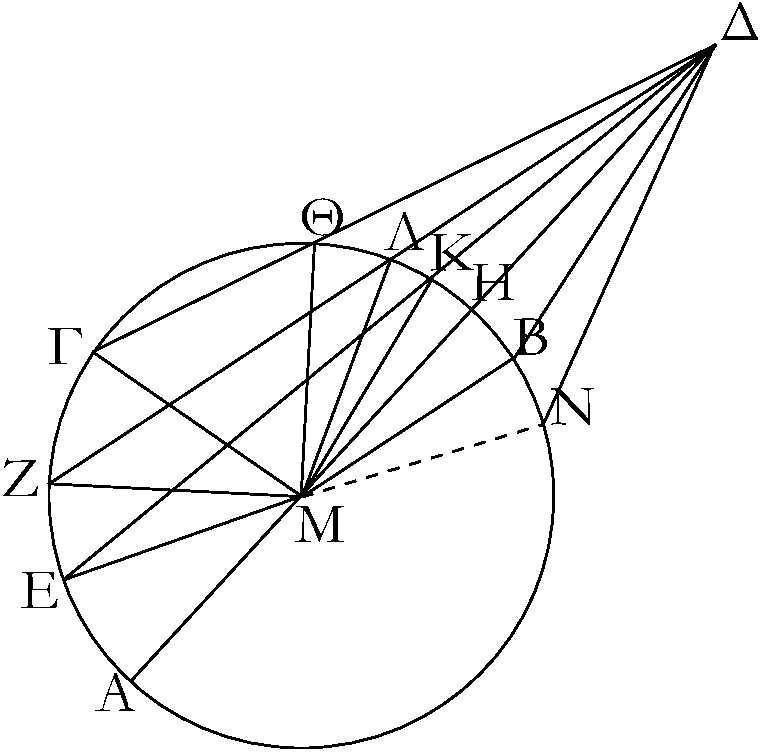
\includegraphics{Book03/fig08g.eps}}

\gr{Λέγω, <ότι καὶ δύο μόνον >ίσαι ἀπὸ τοῦ Δ σημείου προσπεσοῦνται
πρὸξ τὸν κύκλον ἐφ> ἑκάτερα τῆξ ΔΗ ἐλαθίστηξ; συνεστάτω πρὸξ
τῆ| ΜΔ εὐθείᾳ καὶ τῶ| πρὸξ α\kern -.7pt  ὐτῆ| σημείῳ τῶ| Μ τῆ| ὑπὸ ΚΜΔ γωνίᾳ >ίση γωνία ἡ ὑπὸ ΔΜΒ, καὶ ἐπεζεύθθω ἡ ΔΒ. καὶ ἐπεὶ >ίση ἐστὶν ἡ ΜΚ τῆ| ΜΒ, κοινὴ δὲ ἡ ΜΔ, δύο δὴ αἱ ΚΜ, ΜΔ
δύο ταῖξ ΒΜ, ΜΔ >ίσαι εἰσὶν ἑκατέρα ἑκατέρᾳ; καὶ γωνία ἡ
ὑπὸ ΚΜΔ γωνίᾳ τῆ| ὑπὸ ΒΜΔ >ίση; βάσιξ  >άρα ἡ ΔΚ βάσει
τῆ| ΔΒ >ίση ἐστίν. λέγω [δή], <ότι τῆ| ΔΚ εὐθείᾳ >άλλη >ίση
οὐ προσπεσεῖται πρὸξ τὸν κύκλον ἀπὸ τοῦ Δ σημείου. εἰ γὰρ
δυνατόν, προσπιπτέτω καὶ >έστω ἡ ΔΝ. ἐπεὶ ο>ῦν ἡ ΔΚ
τῆ| ΔΝ ἐστιν >ίση, ἀλλ> ἡ ΔΚ τῆ| ΔΒ ἐστιν >ίση, καὶ
ἡ ΔΒ >άρα τῆ| ΔΝ ἐστιν >ίση, ἡ >έγγιον τῆξ ΔΗ ἐλαθίστηξ τῆ|
ἀπώτερον [ἐστιν] >ίση; <όπερ ἀδύνατον ἐδείθθη. οὐκ
>άρα πλείουξ >ὴ δύο >ίσαι πρὸξ τὸν ΑΒΓ κύκλον ἀπὸ τοῦ Δ σημείου
ἐφ> ἑκάτερα τῆξ ΔΗ ἐλαθίστηξ προσπεσοῦνται.}

\gr{Ἐὰν >άρα κύκλου ληφθῆ| τι σημεῖον ἐκτόξ, ἀπὸ δὲ τοῦ σημείου πρὸξ
τὸν κύκλον διαθθῶσιν εὐθεῖαί τινεξ, <ῶν μία μὲν διὰ τοῦ κέντρου
αἱ δὲ λοιπαί, ὡξ >έτυθεν, τῶν μὲν πρὸξ τὴν κοίλην περιφέρειαν προσπιπτουσῶν εὐθειῶν μεγίστη μέν ἐστιν ἡ διὰ τοῦ κέντου, τῶν δὲ >άλλων ἀεὶ ἡ >έγγιον τῆξ διὰ τοῦ κέντρου τῆξ ἀπώτερον μείζων ἐστίν, τῶν δὲ πρὸξ τὴν κυρτὴν περιφέρειαν προσπιπτουσῶν εὐθειῶν
ἐλαθίστη μέν ἐστιν ἡ μεταχὺ τοῦ τε σημείου καὶ τῆξ διαμέτρου, τῶν δὲ >άλλων ἀεὶ ἡ >έγγιον τῆξ ἐλαθίστηξ τῆξ ἀπώτερόν ἐστιν
ἐλάττων, δύο δὲ μόνον >ίσαι ἀπὸ τοῦ σημείου προσπεσοῦνται
πρὸξ τὸν κύκλον ἐφ> ἑκάτερα τῆξ ἐλαθίστηξ; <όπερ >έδει δεῖχαι.}}

\ParallelRText{
\begin{center}
{\large Proposition 8}
\end{center}

If some point is taken outside a circle, and some straight-lines are
drawn from the point to the (circumference of the) circle, one of which (passes) through the
center, the remainder  (being) random, (then) for the straight-lines
radiating towards the concave (part of the) circumference, the
greatest is  that (passing) through the center. For the others, a (straight-line)
nearer$^\dag$ to the (straight-line) through the center is always greater than one
further away. For the straight-lines radiating towards the convex (part of
the) circumference, the least is that between the point and the
diameter. For the others, a (straight-line) nearer to the least
(straight-line) is always less than one further away. And only
two equal (straight-lines) will radiate from the point towards the (circumference of the) circle, (one) on each (side)
of the least (straight-line).

Let $ABC$ be a circle, and let some point $D$ be taken outside $ABC$,
and from it let some straight-lines, $DA$, $DE$, $DF$, and $DC$, be
drawn through (the circle), and let $DA$ be through the center. I say 
that for the straight-lines radiating towards the concave (part of the)
circumference, $AEFC$, the greatest is the one (passing) through the center,  (namely) $AD$,
and (that) $DE$ (is) greater than $DF$, and $DF$ than $DC$. For the straight-lines
radiating towards the convex (part of the) circumference, $HLKG$, the
least is the one between the point and the diameter $AG$, (namely) $DG$, 
and  a (straight-line) nearer to the least (straight-line) $DG$ is
always less than one farther away, (so that) $DK$ (is less) than $DL$, and $DL$ than than
$DH$.

For let the center of the circle be found [Prop.~3.1], and let it be (at point) $M$
[Prop.~3.1]. And let $ME$, $MF$, $MC$, $MK$, $ML$, and $m\kern -.7pt h$ be joined.

And since $AM$ is equal to $EM$, let $MD$ be added to both. Thus, $AD$ is equal to $EM$ and $MD$. But, $EM$ and $MD$ is greater than
$ED$ [Prop.~1.20]. Thus, $AD$ is also greater than $ED$. Again, since $ME$ is
equal to $MF$, and $MD$ (is) common, the (straight-lines) $EM$, $MD$ are thus
equal to $FM$,
$MD$. And angle $EMD$ is greater than angle $FMD$.$^\ddag$
Thus, the
base $ED$ is greater than the base $FD$ [Prop.~1.24]. 
So, similarly,
we can show that $FD$ is also greater than $CD$. Thus, $AD$ (is) the greatest
(straight-line), and $DE$ (is) greater than $DF$, and $DF$ than $DC$.

And since $MK$ and $KD$ is greater than $MD$ [Prop. 1.20], and $MG$ (is)
equal to $MK$, the remainder $KD$ is thus greater than the remainder $GD$.
So $GD$ is less than $KD$. And since in triangle $MLD$, the two internal straight-lines
$MK$ and $KD$ were constructed on one of the sides, $MD$, (then) $MK$ and $KD$
are thus less than $ML$ and $LD$  [Prop.~1.21]. And $MK$ (is) equal to $ML$.
Thus, the remainder $DK$ is less than the remainder $DL$. So, similarly, we
can show that $DL$ is also less than $DH$. Thus, $DG$ (is) the least (straight-line),
and $DK$ (is) less than $DL$, and $DL$ than $DH$.

\epsfysize=2.5in
\centerline{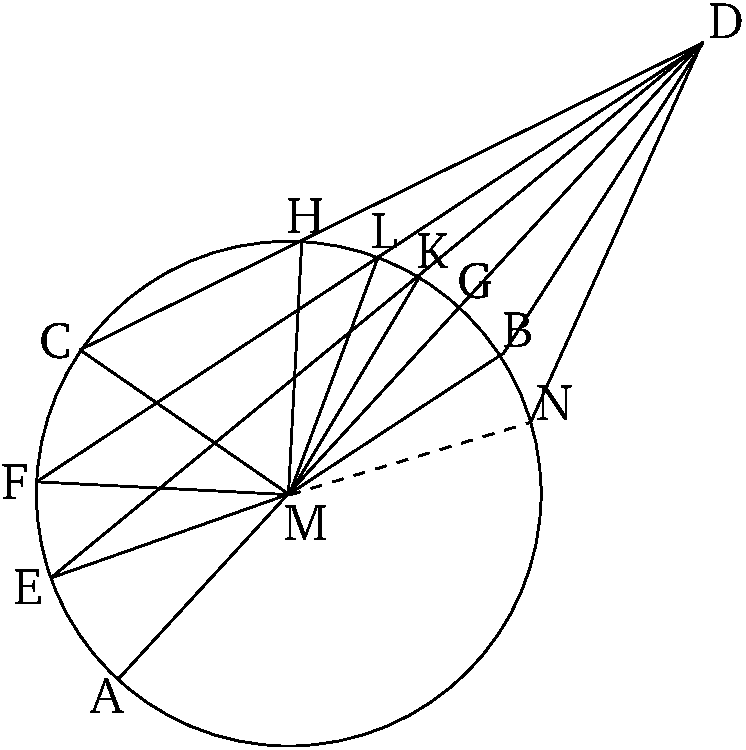
\includegraphics{Book03/fig08e.eps}}

I also say that only two equal (straight-lines) will radiate from point $D$ towards (the
circumference of) the circle, (one) on each (side) on the least (straight-line),
$DG$. Let the  angle $DMB$, equal to angle $KMD$, be constructed
on the straight-line $MD$, at the point $M$ on it [Prop.~1.23], and  let $DB$ be
joined. And since $MK$ is equal to $MB$, and $MD$ (is) common, the
two (straight-lines) $KM$, $MD$ are equal to the two (straight-lines) $BM$, $MD$,
respectively. And angle $KMD$ (is) equal to angle $BMD$. Thus, the base
$DK$ is equal to the base $DB$ [Prop.~1.4]. [So] I say that another (straight-line)
equal to $DK$ will not radiate towards the (circumference of the) circle
from point $D$. For, if possible, let (such a straight-line) radiate, and let
it be $DN$. Therefore, since $DK$ is equal to $DN$, but $DK$ is equal to $DB$, (then) $DB$
is thus also equal to $DN$, (so that) a (straight-line) nearer to the least (straight-line) $DG$ [is]
equal to one further away. The very thing was shown (to be)  impossible. 
Thus, not more than two equal (straight-lines) will radiate towards
(the circumference of) circle $ABC$ from point $D$, (one) on each side
of the least (straight-line) $DG$.

Thus, if some point is taken outside a circle, and some straight-lines are
drawn from the point to the (circumference of the) circle, one of which (passes) through the
center, the remainder  (being) random, (then) for the straight-lines
radiating towards the concave (part of the) circumference, the
greatest is  that (passing) through the center. For the others, a (straight-line)
nearer to the (straight-line) through the center is always greater than one
further away. For the straight-lines radiating towards the convex (part of
the) circumference, the least is that between the point and the
diameter. For the others, a (straight-line) nearer to the least
(straight-line) is always less than one further away. And only
two equal (straight-lines) will radiate from the point towards the (circumference of the) circle, (one) on each (side)
of the least (straight-line).  (Which is) the very thing it was required to show.}
\end{Parallel}
{\footnotesize \noindent$^\dag$ Presumably, in an angular sense.\\
$\ddag$  This is not
proved, except by reference to the figure.} 

%%%%%%
% Prop 3.9
%%%%%%
\pdfbookmark[1]{Proposition 3.9}{pdf3.9}
\begin{Parallel}{}{} 
\ParallelLText{
\begin{center}
{\large \ggn{9}.}
\end{center}\vspace*{-7pt}

\gr{Ἐὰν κύκλου ληφθῆ| τι σημεῖον ἐντόξ, ἀπο δὲ τοῦ σημείου πρὸξ
τὸν κύκλον προσπίπτωσι πλείουξ >ὴ δύο >ίσαι εὐθεῖαι, τὸ ληφθὲν σημεῖον κέντρον ἐστὶ τοῦ κύκλου.}

\gr{>'Εστω κύκλοξ ὁ ΑΒΓ, ἐντὸξ δὲ α\kern -.7pt  ὐτοῦ σημεῖον τὸ Δ, καὶ ἀπὸ
τοῦ Δ πρὸξ τὸν ΑΒΓ κύκλον προσπιπτέτωσαν πλείουξ >ὴ δύο >ίσαι
εὐθεῖαι αἱ ΔΑ, ΔΒ, ΔΓ; λέγω, <ότι τὸ Δ σημεῖον κέντρον ἐστὶ τοῦ
ΑΒΓ κύκλου.}\\

\epsfysize=2.2in
\centerline{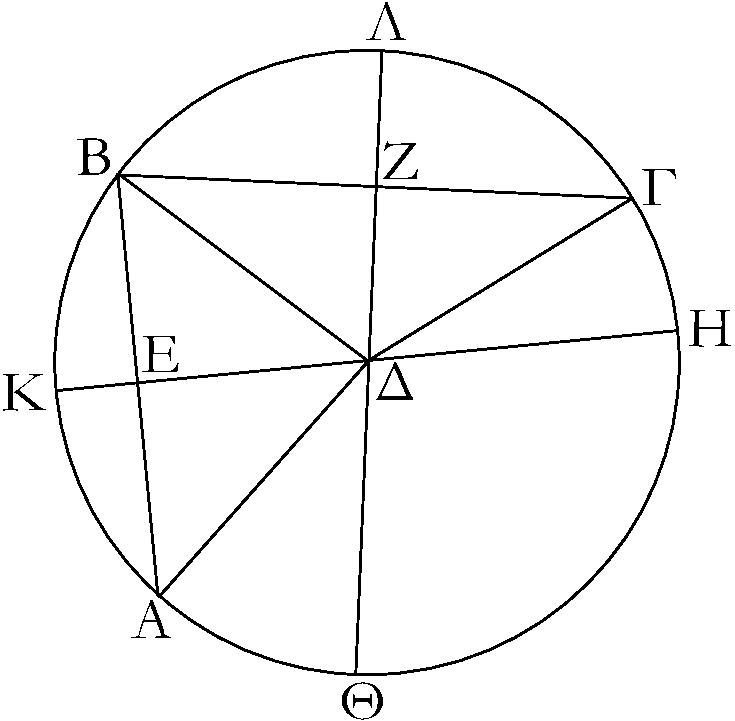
\includegraphics{Book03/fig09g.eps}}

\gr{Ἐπεζεύθθωσαν γὰρ αἱ ΑΒ, ΒΓ καὶ τετμ\kern -.7pt  ήσθωσαν δίθα κατὰ τὰ Ε, Ζ σημεῖα, καὶ ἐπιζευθθεῖσαι αἱ ΕΔ, ΖΔ διήθθωσαν ἐπὶ τὰ
Η, Κ, J, Λ σημεῖα.}

\gr{Ἐπεὶ ο>ῦν >ίση ἐστὶν ἡ ΑΕ τῆ| ΕΒ, κοινὴ δὲ ἡ ΕΔ,
δύο δὴ αἱ ΑΕ, ΕΔ δύο ταῖξ ΒΕ, ΕΔ >ίσαι εἰσίν; καὶ βάσιξ ἡ
ΔΑ βάσει τῆ| ΔΒ >ίση; γωνία >άρα ἡ ὑπὸ ΑΕΔ γωνίᾳ
τῆ| ὑπὸ ΒΕΔ >ίση ἐστίν; ὀρθὴ >άρα ἑκατέρα τῶν ὑπὸ ΑΕΔ,
ΒΕΔ γωνιῶν; ἡ ΗΚ >άρα τὴν ΑΒ τέμνει δίθα καὶ πρὸξ ὀρθάξ. καὶ
ἐπεί, ἒαν ἐν κύκλῳ εὐθεῖά τιξ εὐθεῖάν τινα δίθα τε καὶ πρὸξ
ὀρθὰξ τέμνῃ, ἐπὶ τῆξ τεμνούσηξ ἐστὶ τὸ κέντρον τοῦ κύκλου,
ἐπὶ τῆξ ΗΚ >άρα ἐστὶ τὸ κέντρον τοῦ κύκλου. διὰ τὰ
α\kern -.7pt  ὐτὰ δὴ καὶ ἐπὶ τῆξ JΛ ἐστι τὸ κέντρον τοῦ ΑΒΓ κύκλου.
καὶ οὐδὲν <έτερον κοινὸν >έθουσιν αἱ ΗΚ, JΛ εὐθεῖαι >ὴ τὸ Δ
σημεῖον; τὸ Δ >άρα σημεῖον κέντρον ἐστὶ τοῦ ΑΒΓ
κύκλου.}

\gr{Ἐὰν >άρα κύκλου ληφθῆ| τι σημεῖον ἐντόξ, ἀπὸ δὲ τοῦ σημείου πρὸξ
τὸν κύκλον προσπίπτωσι πλείουξ >ὴ δύο >ίσαι εὐθεῖαι, τὸ ληφθὲν σημεῖον κέντρον ἐστὶ τοῦ κύκλου; <όπερ >έδει δεῖχαι.}}

\ParallelRText{
\begin{center}
{\large Proposition 9}
\end{center}

If  some point is taken inside a circle, and more than two equal straight-lines
radiate from the point towards the (circumference of the) circle, (then) the
point taken  is the center of the circle.

Let $ABC$ be a circle, and $D$ a point inside it, and let more than two equal
straight-lines, $DA$, $DB$, and $DC$, radiate from $D$ towards (the circumference of) circle
$ABC$. I say that point $D$ is the center of circle $ABC$.

\epsfysize=2.2in
\centerline{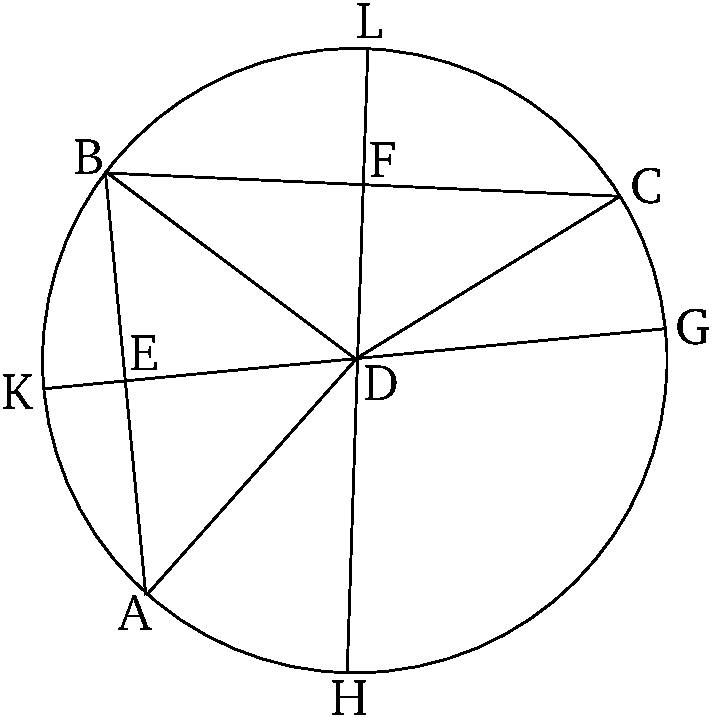
\includegraphics{Book03/fig09e.eps}}

For let $AB$ and $BC$ be joined, and (then) be cut in half at points $E$ and $F$ 
(respectively) [Prop.~1.10]. And $ED$ and $FD$ being joined, let them be
drawn through to points $G$, $K$, $H$, and $L$.

Therefore, since $AE$ is equal to $EB$, and $ED$ (is) common, the two (straight-lines) $AE$, $ED$ are equal to the two (straight-lines) $BE$, $ED$ (respectively). And the 
base $DA$ (is) equal to the base $DB$. Thus, angle $AED$ is equal to
angle $BED$ [Prop.~1.8]. Thus, angles $AED$ and $BED$ (are) each right-angles [Def.~1.10]. Thus, $GK$ cuts $AB$ in half, and at right-angles. And since,
if some straight-line in a circle cuts some (other) straight-line in half,
and at right-angles, (then) the center of the circle is on the former (straight-line)
[Prop.~3.1~corr.], the center of the circle is thus on $GK$. So, for the
same (reasons), the center of circle $ABC$ is also on $HL$. And the straight-lines
$GK$ and $HL$ have no  common (point) other than point $D$. Thus, point
$D$ is the center of circle $ABC$.

Thus, if some point is taken inside a circle, and more than two equal straight-lines
radiate from the point towards the (circumference of the) circle, (then) the
point taken  is the center of the circle. (Which is) the very thing it was
required to show.}
\end{Parallel}

%%%%%%
% Prop 3.10
%%%%%%
\pdfbookmark[1]{Proposition 3.10}{pdf3.10}
\begin{Parallel}{}{} 
\ParallelLText{
\begin{center}
{\large \ggn{10}.}
\end{center}\vspace*{-7pt}

\gr{Κύκλοξ  κύκλον οὐ τέμνει κατὰ πλείονα σημεῖα >ὴ δύο.}

\gr{Εἰ γὰρ δυνατόν, κύκλοξ ὁ ΑΒΓ κύκλον τὸν ΔΕΖ τεμνέτω κατὰ πλείονα
σημεῖα >ὴ δύο τὰ Β, Η, Ζ, J, καὶ ἐπιζευθθεῖσαι αἱ ΒJ, ΒΗ δίθα τεμνέσθωσαν κατὰ τὰ Κ, Λ σημεῖα; καὶ ἀπὸ τῶν Κ, Λ ταῖξ ΒJ, ΒΗ
πρὸξ ὀρθὰξ ἀθθεῖσαι αἱ ΚΓ, ΛΜ διήθθωσαν ἐπὶ τὰ Α, Ε σημεῖα.}\\~\\

\epsfysize=2.2in
\centerline{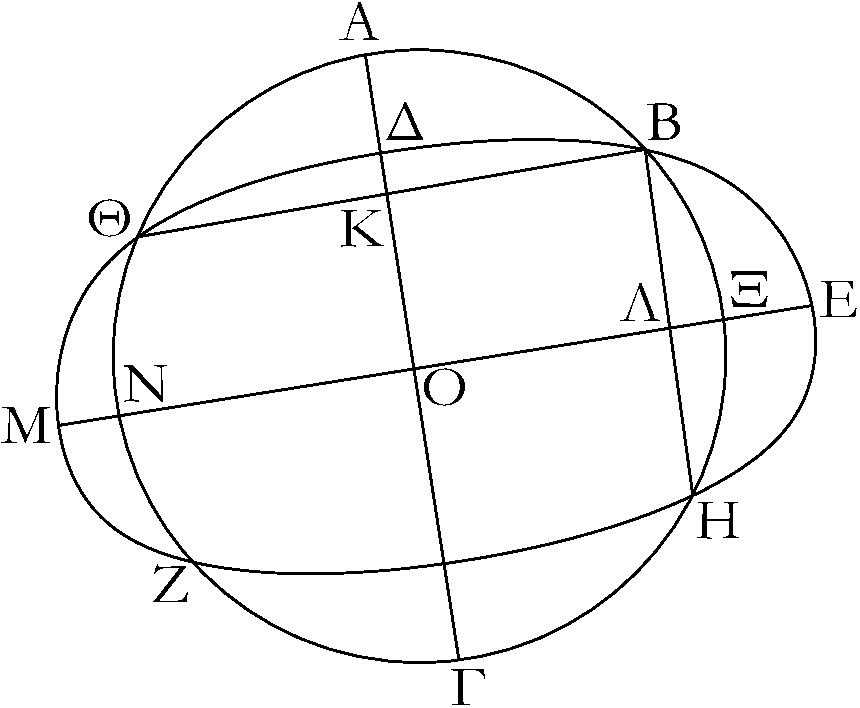
\includegraphics{Book03/fig10g.eps}}

\gr{Ἐπεὶ ο>ῦν ἐν κύκλῳ τῶ| ΑΒΓ εὐθεῖά τιξ ἡ ΑΓ εὐθεῖάν τινα
τὴν ΒJ δίθα καὶ πρὸξ ὀρθὰξ τέμνει, ἐπὶ τῆξ ΑΓ >άρα ἐστὶ τὸ κέντρον τοῦ ΑΒΓ κύκλου. πάλιν, ἐπεὶ ἐν κύκλῳ τῶ| α\kern -.7pt  ὐτῶ|
τῶ| ΑΒΓ εὐθεῖά τιξ ἡ ΝΧ εὐθεῖάν τινα τὴν ΒΗ δίθα καὶ πρὸξ
ὀρθὰξ τέμνει, ἐπὶ τῆξ ΝΧ >άρα ἐστὶ τὸ κέντρον τοῦ ΑΒΓ κύκλου.
ἐδείθθη δὲ καὶ ἐπὶ τῆξ ΑΓ, καὶ κατ> οὐδὲν συμβάλλουσιν
αἱ ΑΓ, ΝΧ εὐθεῖαι >ὴ κατὰ τὸ Ο; τὸ Ο >άρα σημεῖον κέντρον
ἐστὶ τοῦ ΑΒΓ κύκλου. ὁμοίωξ δὴ δείχομεν, <ότι καὶ τοῦ ΔΕΖ κύκλου κέντρον ἐστὶ τὸ Ο; δύο >άρα κύκλων τεμνόντων ἀλλήλουξ
τῶν ΑΒΓ, ΔΕΖ τὸ α\kern -.7pt  ὐτό ἐστι κέντρον τὸ Ο; 
<όπερ ἐστὶν ἀδύνατον.}

\gr{Οὐκ >άρα κύκλοξ  κύκλον τέμνει κατὰ πλείονα σημεῖα >ὴ δύο;
<όπερ >έδει δεῖχαι.}}

\ParallelRText{
\begin{center}
{\large Proposition 10}
\end{center}

A circle does not cut a(nother) circle at more than two points.

For, if possible, let the circle $ABC$ cut the circle $DEF$ at more than
two points, $B$, $G$, $F$, and $H$. And $BH$ and $BG$ being joined,
let them (then) be cut in half at points $K$ and $L$ (respectively). And $KC$ and $LM$
being drawn at right-angles to $BH$ and $BG$ from $K$ and $L$ (respectively) [Prop.~1.11], let them (then) be
drawn through to points $A$ and $E$ (respectively).

\epsfysize=2.2in
\centerline{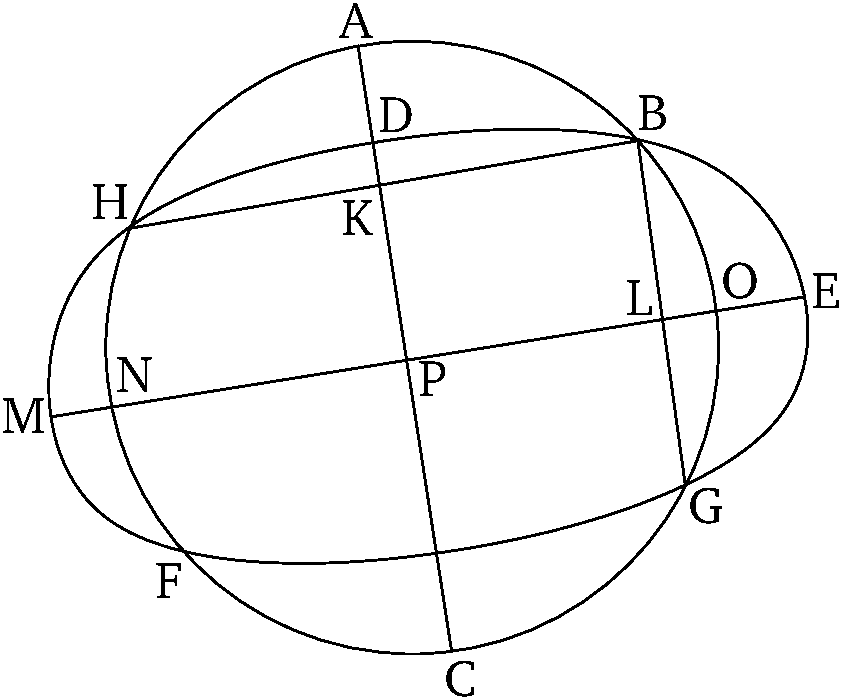
\includegraphics{Book03/fig10e.eps}}

Therefore, since in circle $ABC$ some straight-line $AC$ cuts some (other)
straight-line $BH$ in half, and at right-angles, the center of circle $ABC$
is thus on $AC$ [Prop.~3.1~corr.]. Again, since in the same circle $ABC$
some straight-line $NO$ cuts some (other straight-line) $BG$ in half, and
at right-angles, the center of circle $ABC$ is thus on $NO$ [Prop.~3.1~corr.].
And it was also shown (to be) on $AC$. And the straight-lines $AC$ and $NO$
meet at no other (point) than $P$. Thus, point $P$ is the center of circle $ABC$.
So, similarly, we can show that $P$ is also the center of circle $DEF$.
Thus,  two circles cutting one another, $ABC$ and $DEF$, have the same center
$P$. The very thing is impossible [Prop.~3.5].

Thus, a circle does not cut a(nother) circle at more than two points. (Which is)
the very thing it was required to show.}
\end{Parallel}

%%%%%%
% Prop 3.11
%%%%%%
\pdfbookmark[1]{Proposition 3.11}{pdf3.11}
\begin{Parallel}{}{} 
\ParallelLText{
\begin{center}
{\large \ggn{11}.}
\end{center}\vspace*{-7pt}

\gr{Ἐὰν δύο κύκλοι ἐφάπτωνται ἀλλήλων ἐντόξ, καὶ ληφθῆ| α\kern -.7pt  ὐτῶν
τὰ κέντρα, ἡ ἐπὶ τὰ κέντρα α\kern -.7pt  ὐτῶν ἐπιζευγνυμένη εὐθεῖα καὶ
ἐκβαλλομένη ἐπὶ τὴν συναφὴν πεσεῖται τῶν κύκλων.}

\gr{Δύο γὰρ κύκλοι οἱ ΑΒΓ, ΑΔΕ ἐφαπτέσθωσαν ἀλλήλων ἐντὸξ κατὰ τὸ
Α σημεῖον, καὶ εἰλήφθω τοῦ μὲν ΑΒΓ κύκλου κέντρον τὸ Ζ, τοῦ δὲ
ΑΔΕ τὸ Η; λέγω, <ότι ἡ ἀπὸ τοῦ Η ἐπὶ τὸ Ζ ἐπιζευγνυμένη
εὐθεῖα ἐκβαλλομένη ἐπὶ τὸ Α πεσεῖται.}

\gr{μ\kern -.7pt  ὴ γάρ, ἀλλ> εἰ δυνατόν, πιπτέτω ὡξ ἡ ΖΗJ, καὶ
ἐπεζεύθθωσαν αἱ ΑΖ, ΑΗ.}

\gr{Ἐπεὶ ο>ῦν αἱ ΑΗ, ΗΖ τῆξ ΖΑ, τουτέστι τῆξ ΖJ, μείζονέξ εἰσιν, 
κοινὴ ἀφῃρήσθω ἡ ΖΗ; λοιπὴ >άρα ἡ ΑΗ λοιπῆξ τῆξ ΗJ μείζων ἐστίν. >ίση δὲ ἡ ΑΗ τῆ| ΗΔ; καὶ ἡ ΗΔ >άρα τῆξ ΗJ μείζων ἐστὶν
ἡ ἐλάττων τῆξ μείζονοξ; <όπερ ἐστὶν ἀδύνατον; οὐκ >άρα ἡ ἀπὸ
τοῦ Ζ ἐπὶ τὸ Η ἐπιζευγνυμένη εὐθεὶα ἐκτὸξ πεσεῖται;
κατὰ τὸ Α >άρα ἐπὶ τῆξ συναφῆξ πεσεῖται.}\\~\\

\epsfysize=2.2in
\centerline{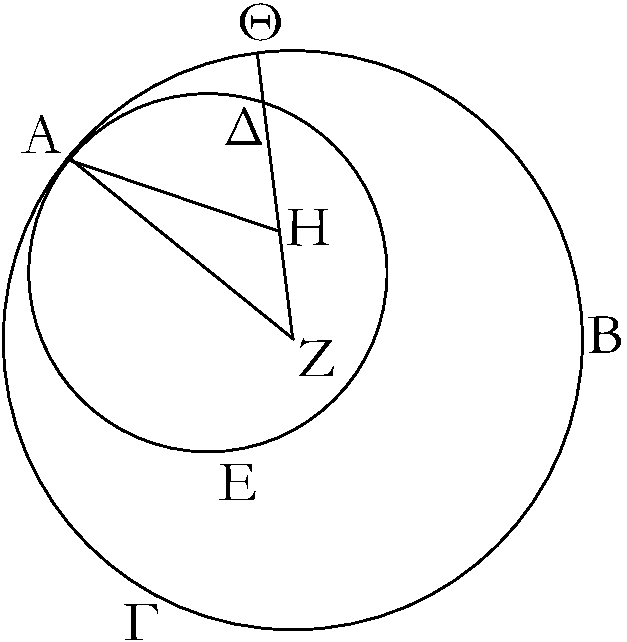
\includegraphics{Book03/fig11g.eps}}

\gr{Ἐὰν >άρα δύο κύκλοι ἐφάπτωνται ἀλλήλων ἐντόξ, [καὶ ληφθῆ| α\kern -.7pt  ὐτῶν
τὰ κέντρα], ἡ ἐπὶ τὰ κέντρα α\kern -.7pt  ὐτῶν ἐπιζευγνυμένη εὐθεῖα [καὶ
ἐκβαλλομένη] ἐπὶ τὴν συναφὴν πεσεῖται τῶν κύκλων; <όπερ
>έδει δεῖχαι.}}

\ParallelRText{
\begin{center}
{\large Proposition 11}
\end{center}

If two circles  touch one another internally, and their
centers are found, (then)  the straight-line joining their
centers, being produced, will fall upon the point of union of
the circles.

For let two circles, $ABC$ and $ADE$, touch one another internally
at point $A$, and let the center $F$ of circle $ABC$ be
found [Prop.~3.1], and (the center) $G$ of (circle) $ADE$ [Prop.~3.1].
I say that the straight-line joining $G$ to $F$, being produced, will fall on $A$.

For (if) not (then), if possible, let it fall like $FGH$ (in the figure), and
let $AF$ and $AG$ be joined.

Therefore, since $AG$ and $GF$ is greater than $FA$, that is to
say $FH$ [Prop.~1.20], let $FG$ be taken from both.
Thus, the remainder $AG$ is greater than the remainder $GH$.
And $AG$ (is) equal to $GD$. Thus, $GD$ is also greater than $GH$, the lesser
than the greater. The very thing is impossible. Thus, the straight-line
joining $F$ to $G$ will not fall outside (one circle but inside the other). Thus, it will fall upon the point of
union (of the circles) at point $A$. 

\epsfysize=2.2in
\centerline{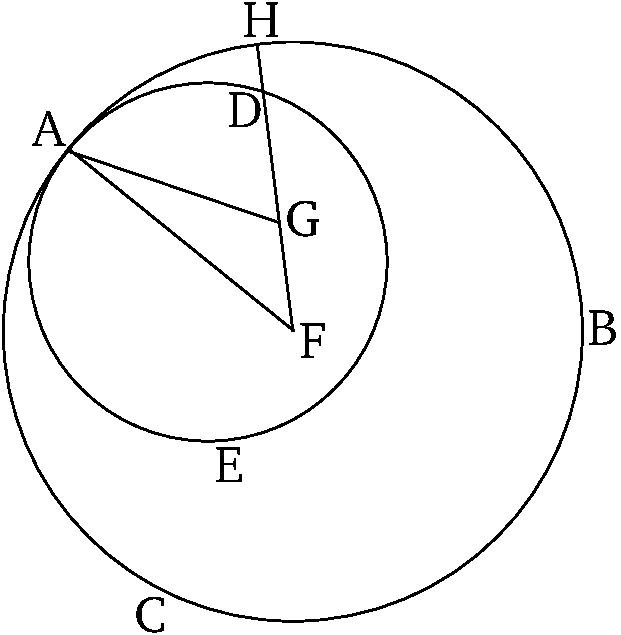
\includegraphics{Book03/fig11e.eps}}

Thus, if two circles  touch one another internally, [and their
centers are found], (then)  the straight-line joining their
centers, [being produced], will fall upon the point of union of
the circles. (Which is) the very thing it was required to show.}
\end{Parallel}

%%%%%%
% Prop 3.12
%%%%%%
\pdfbookmark[1]{Proposition 3.12}{pdf3.12}
\begin{Parallel}{}{} 
\ParallelLText{
\begin{center}
{\large \ggn{12}.}
\end{center}\vspace*{-7pt}

\gr{Ἐὰν δύο κύκλοι ἐφάπτωνται ἀλλήλων ἐκτόξ, ἡ ἐπὶ τὰ κέντρα
α\kern -.7pt  ὐτῶν ἐπιζευγνυμένη διὰ τῆξ ἐπαφῆξ ἐλεύσεται.}\\

\epsfysize=2.5in
\centerline{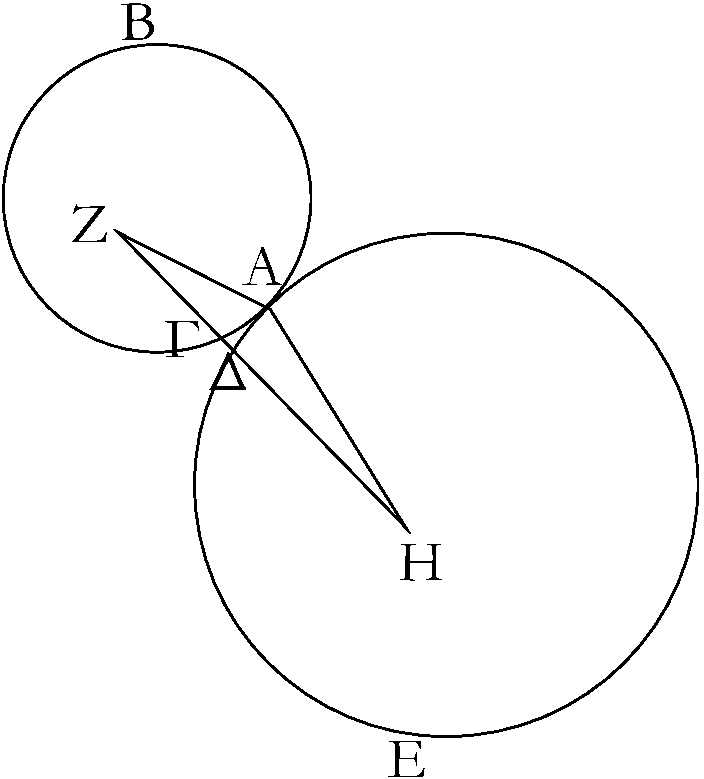
\includegraphics{Book03/fig12g.eps}}

\gr{Δύο γὰρ κύκλοι οἱ ΑΒΓ, ΑΔΕ ἐφαπτέσθωσαν ἀλλήλων ἐκτὸξ
κατὰ τὸ Α σημεῖον, καὶ εἰλήφθω τοῦ μὲν ΑΒΓ κέντρον τὸ Ζ,
τοῦ δὲ ΑΔΕ τὸ Η; λέγω, <ότι ἡ ἀπὸ τοῦ Ζ ἐπὶ τὸ Η
ἐπιζευγνυμένη εὐθεῖα διὰ τῆξ κατὰ τὸ Α ἐπαφῆξ ἐλεύσεται.}

\gr{μ\kern -.7pt  ὴ γάρ, ἀλλ> εἰ δυνατόν, ἐρθέσθω ὡξ ἡ ΖΓΔΗ, καὶ ἐπεζεύθθωσαν
αἱ ΑΖ, ΑΗ.}

\gr{Ἐπεὶ ο>ῦν τὸ Ζ σημεῖον κέντρον ἐστὶ τοῦ ΑΒΓ κύκλου,
>ίση ἐστὶν ἡ ΖΑ τῆ| ΖΓ. πάλιν, ἐπεὶ τὸ Η σημεῖον κέντρον
ἐστὶ τοῦ ΑΔΕ κύκλου, >ίση ἐστὶν ἡ ΗΑ τῆ| ΗΔ. ἐδείθθη δὲ
καὶ ἡ ΖΑ τῆ| ΖΓ >ίση; αἱ >άρα ΖΑ, ΑΗ ταῖξ ΖΓ, ΗΔ >ίσαι εἰσίν; <ώστε <όλη ἡ ΖΗ τῶν ΖΑ, ΑΗ μείζων ἐστίν; ἀλλὰ καὶ ἐλάττων;
<όπερ ἐστὶν ἀδύνατον. οὐκ >άρα ἡ ἀπὸ τοῦ Ζ ἐπὶ τὸ Η
ἐπιζευγνυμένη εὐθεῖα διὰ τῆξ κατὰ τὸ Α ἐπαφῆξ οὐκ ἐλεύσεται;
δι> α\kern -.7pt  ὐτῆξ >άρα.}

\gr{Ἐὰν >άρα δύο κύκλοι ἐφάπτωνται ἀλλήλων ἐκτόξ, ἡ ἐπὶ τὰ κέντρα
α\kern -.7pt  ὐτῶν ἐπιζευγνυμένη [εὐθεῖα] διὰ τῆξ ἐπαφῆξ ἐλεύσεται; <όπερ
>έδει δεῖχαι.}}

\ParallelRText{
\begin{center}
{\large Proposition 12}
\end{center}

If two circles touch one another externally, (then) the (straight-line)
joining their centers will go through the point of union.

\epsfysize=2.5in
\centerline{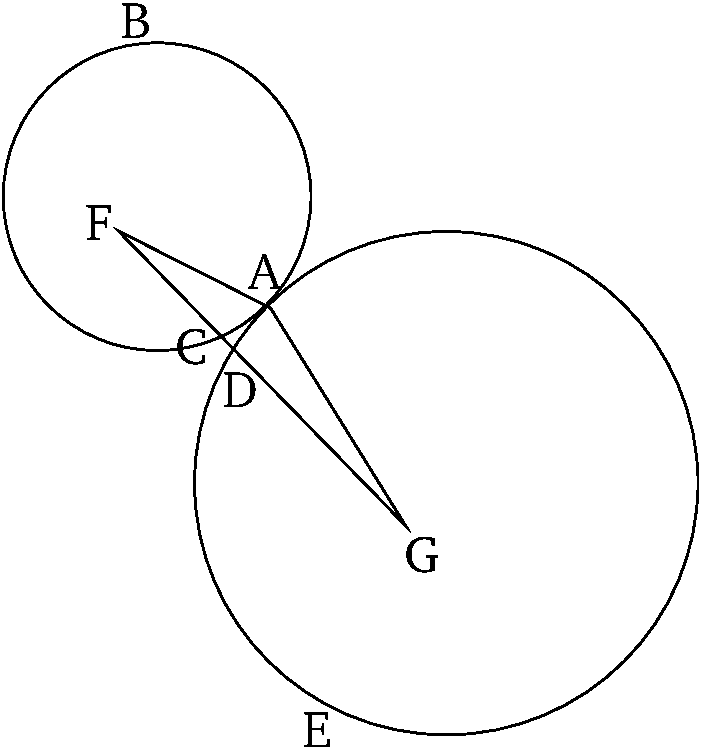
\includegraphics{Book03/fig12e.eps}}

For let two circles, $ABC$ and $ADE$, touch one another externally at point $A$,
and let the center $F$ of $ABC$ be found [Prop.~3.1], and
(the center) $G$ of $ADE$ [Prop.~3.1]. I say that the straight-line joining
$F$ to $G$ will go through the point of union at $A$.

For (if) not (then), if possible, let it go like $FCDG$ (in the figure), and let $AF$ and
$AG$ be joined.

Therefore, since point $F$ is the center of circle $ABC$, $FA$ is equal to $FC$.
Again, since point $G$ is the center of circle $ADE$, $GA$ is equal to $GD$.
And $FA$ was also shown (to be)  equal to $FC$. Thus, the (straight-lines)
$FA$ and $AG$ are equal to the (straight-lines) $FC$ and $GD$. So the whole
of $FG$ is greater than $FA$ and $AG$. But, (it is) also less [Prop.~1.20].
The very thing is impossible. Thus, the straight-line joining $F$ to $G$
cannot not go through the point of union at $A$. Thus, (it will go) through it.

Thus, if two circles touch one another externally, (then) the [straight-line]
joining their centers will go through the point of union. (Which is)
the very thing it was required to show.}
\end{Parallel}

%%%%%%
% Prop 3.13
%%%%%%
\pdfbookmark[1]{Proposition 3.13}{pdf3.13}
\begin{Parallel}{}{} 
\ParallelLText{
\begin{center}
{\large \ggn{13}.}
\end{center}\vspace*{-7pt}

\gr{Κύκλοξ κύκλου οὐκ ἐφάπτεται κατὰ πλείονα σημεῖα
>ὴ  καj> <έν, ἔαν τε ἐντὸξ ἔαν τε ἐκτὸξ ἐφάπτηται.}

\epsfysize=2.2in
\centerline{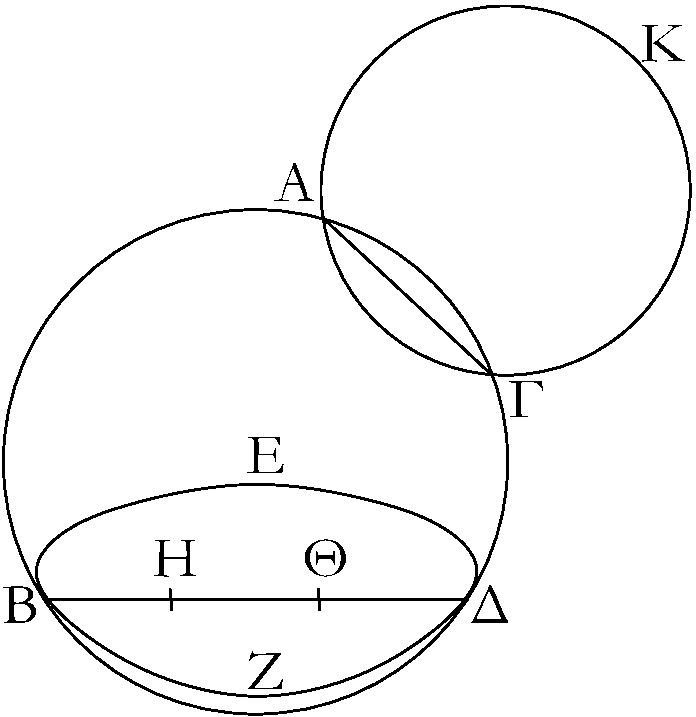
\includegraphics{Book03/fig13g.eps}}

\gr{Εἰ γὰρ δυνατόν, κύκλοξ ὁ ΑΒΓΔ κύκλου τοῦ ΕΒΖΔ ἐφαπτέσθω
πρότερον ἐντὸξ κατὰ πλείονα σημεῖα >ὴ <ὲν τὰ Δ, Β.}

\gr{Καὶ εἰλήφθω τοῦ μὲν ΑΒΓΔ κύκλου κέντρον τὸ Η, τοῦ δὲ ΕΒΖΔ
τὸ J.}

\gr{Ἡ >άρα ἀπὸ τοῦ Η ἐπὶ τὸ J ἐπιζευγνυμένη ἐπὶ τὰ Β, Δ πεσεῖται.
πιπτέτω ὡξ ἡ ΒΗJΔ. καὶ ἐπεὶ τὸ Η σημεῖον κέντρον ἐστὶ τοῦ
ΑΒΓΔ κύκλου, >ίση ἐστὶν ἡ ΒΗ τῆ| ΗΔ; μείζων >άρα ἡ ΒΗ τῆξ
JΔ; πολλῶ| >άρα μείζων ἡ ΒJ τῆξ JΔ. πάλιν, ἐπεὶ τὸ J σημεῖον
κέντρον ἐστὶ τοῦ ΕΒΖΔ κύκλου, >ίση ἐστὶν ἡ ΒJ τῆ| JΔ;
ἐδείθθη δὲ α\kern -.7pt  ὐτῆξ καὶ πολλῶ| μείζων; <όπερ ἀδύνατον;
οὐκ >άρα κύκλοξ κύκλου ἐφάπτεται ἐντὸξ κατὰ πλείονα σημεῖα
>ὴ <έν.}

\gr{Λέγω δή, <ότι οὐδὲ ἐκτόξ.}

\gr{Εἰ γὰρ δυνατόν, κύκλοξ ὁ ΑΓΚ κύκλου τοῦ ΑΒΓΔ ἐφαπτέσθω ἐκτὸξ
κατὰ πλείονα σημεῖα >ὴ <ὲν τὰ Α, Γ, καὶ ἐπεζεύθθω ἡ ΑΓ.}

\gr{>'Επεὶ ο>ῦν κύκλων τῶν ΑΒΓΔ, ΑΓΚ ε>ίληπται ἐπὶ
τῆξ περιφερείαξ ἑκατέρου δύο τυθόντα σημεῖα τὰ Α, Γ, ἡ
ἐπὶ τὰ σημεῖα ἐπιζευγνυμένη εὐθεῖα ἐντὸξ ἑκατέρου πεσεῖται;
ἀλλὰ τοῦ μὲν ΑΒΓΔ ἐντὸξ >έπεσεν, τοῦ δὲ ΑΓΚ ἐκτόξ; <όπερ
>άτοπον; οὐκ >άρα κύκλοξ κύκλου ἐφάπτεται ἐκτὸξ κατὰ πλείονα
σημεῖα >ὴ <έν. ἐδείθθη δέ, <ότι οὐδὲ ἐντόξ.}

\gr{Κύκλοξ >άρα κύκλου οὐκ ἐφάπτεται κατὰ πλείονα σημεῖα >ὴ
[καj>] <έν, ἔαν τε ἐντὸξ ἔαν τε ἐκτὸξ ἐφάπτηται; <όπερ >έδει
δεῖχαι.}}

\ParallelRText{
\begin{center}
{\large Proposition 13}
\end{center}

A circle does not touch a(nother) circle at more than one point, whether they
touch internally or externally.

\epsfysize=2.2in
\centerline{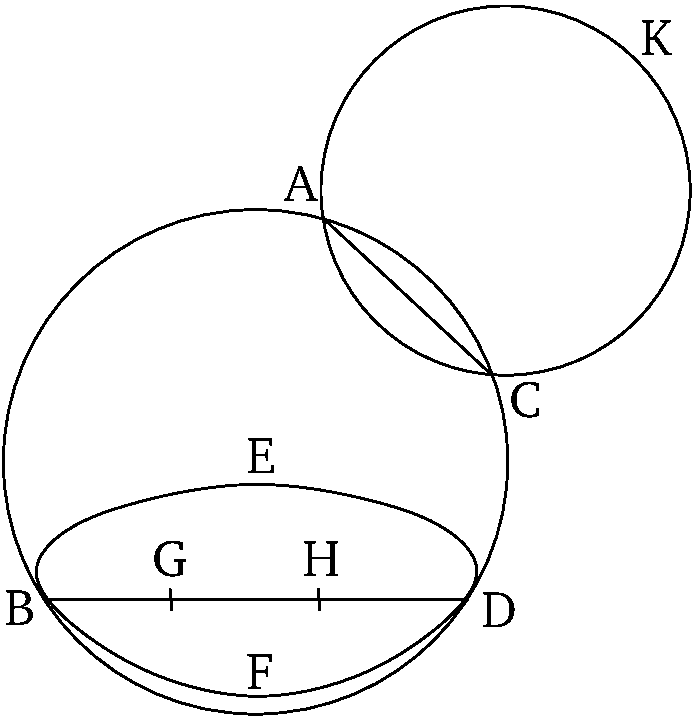
\includegraphics{Book03/fig13e.eps}}

For, if possible, let circle $ABDC$$^{\,\dag}$ touch circle $EBFD$---first of all, internally---at more than one point, $D$ and $B$.

And let the center $G$ of circle $ABDC$ be found [Prop.~3.1], and
(the center) $H$ of $EBFD$ [Prop.~3.1].

Thus, the (straight-line) joining $G$ and $H$ will fall on $B$ and $D$ [Prop.~3.11].
Let it fall like $BGHD$ (in the figure). And since point $G$ is the center of
circle $ABDC$, $BG$ is  equal to $GD$. Thus, $BG$ (is) greater than $HD$.
Thus, $BH$ (is) much greater than $HD$. Again, since point $H$ is the
center of circle $EBFD$, $BH$ is equal to $HD$. But it was also shown
(to be) much greater than it. The very thing (is) impossible.
Thus, a circle does not touch a(nother) circle internally at more than one point.

So, I say that neither (does it touch) externally (at more than one point).

For, if possible, let circle $ACK$ touch circle $ABDC$ externally at more
than one point, $A$ and $C$. And let $AC$ be joined.

Therefore, since  two points, $A$ and $C$,
be taken at random on the circumference
of each of the circles $ABDC$ and $ACK$, the straight-line joining
the points will fall inside each (circle) [Prop.~3.2]. But, it fell
inside $ABDC$, and outside $ACK$ [Def.~3.3]. The very thing (is) absurd.
Thus, a circle does not touch a(nother) circle externally  at more than one
point. And it was shown that neither (does it) internally.

Thus, a circle does not touch a(nother) circle at more than one point, whether they touch internally or externally. (Which is) the very thing it was required to
show.}
\end{Parallel}
{\footnotesize \noindent$^\dag$ The Greek text has ``$ABCD$'', which is obviously a mistake.}

%%%%%%
% Prop 3.14
%%%%%%
\pdfbookmark[1]{Proposition 3.14}{pdf3.14}
\begin{Parallel}{}{} 
\ParallelLText{
\begin{center}
{\large \ggn{14}.}
\end{center}\vspace*{-7pt}

\gr{Ἐν κύκλῳ αἱ >ίσαι εὐθεῖαι >ίσον ἀπέθουσιν ἀπὸ τοῦ κέντρου, καὶ
αἱ >ίσον ἀπέθουσαι ἀπὸ τοῦ κέντρου >ίσαι ἀλλήλαιξ εἰσίν.}\\

\epsfysize=2.2in
\centerline{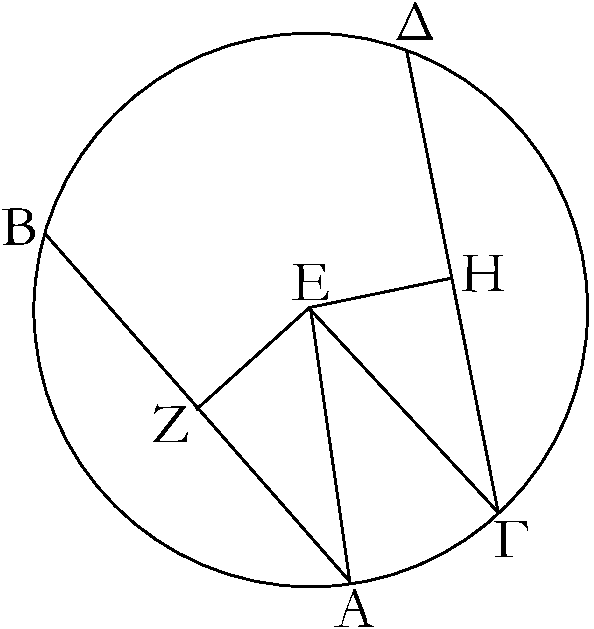
\includegraphics{Book03/fig14g.eps}}

\gr{>'Εστω κύκλοξ ὁ ΑΒΓΔ, καὶ ἐν α\kern -.7pt  ὐτῶ| >ίσαι εὐθεῖαι >έστωσαν αἱ
ΑΒ, ΓΔ; λέγω, <ότι αἱ ΑΒ, ΓΔ >ίσον ἀπέθουσιν ἀπὸ τοῦ
κέντρου.}

\gr{Εἰλήφθω γὰρ τὸ κέντον τοῦ ΑΒΓΔ κύκλου καὶ >έστω τὸ Ε, καὶ
ἀπὸ τοῦ Ε ἐπὶ τὰξ ΑΒ, ΓΔ κάθετοι >ήθθωσαν αἱ ΕΖ, ΕΗ, καὶ
ἐπεζεύθθωσαν αἱ ΑΕ, ΕΓ.}

\gr{Ἐπεὶ ο>ῦν εὐθεῖά τιξ δὶα τοῦ κέντρου ἡ ΕΖ εὐθεῖάν τινα μ\kern -.7pt  ὴ
διὰ τοῦ κέντρου τὴν ΑΒ πρὸξ ὀρθὰξ τέμνει, καὶ δίθα α\kern -.7pt  ὐτὴν
τέμνει. >ίση >άρα ἡ ΑΖ τῆ| ΖΒ; διπλῆ >άρα ἡ ΑΒ τῆξ ΑΖ. διὰ τὰ
α\kern -.5pt  ὐτὰ δὴ καὶ ἡ ΓΔ τῆξ ΓΗ ἐστι διπλῆ; καί ἐστιν >ίση ἡ ΑΒ
τῆ| ΓΔ; >ίση >άρα καὶ ἡ ΑΖ τῆ| ΓΗ. καὶ ἐπεὶ >ίση ἐστὶν ἡ ΑΕ
τῆ| ΕΓ, >ίσον καὶ τὸ ἀπὸ τῆξ ΑΕ τῶ| ἀπὸ τῆξ ΕΓ.
ἀλλὰ τῶ| μὲν ἀπὸ τῆξ ΑΕ >ίσα τὰ ἀπὸ τῶν ΑΖ, ΕΖ; ὀρθὴ γὰρ ἡ πρὸξ τῶ| Ζ γωνία; τῶ| δὲ ἀπὸ τῆξ ΕΓ >ίσα τὰ ἀπὸ τῶν ΕΗ, ΗΓ;
ὀρθὴ γὰρ ἡ πρὸξ τῶ| Η γωνία; τὰ >άρα ἀπὸ τῶν ΑΖ, ΖΕ >ίσα
ἐστὶ τοῖξ ἀπὸ τῶν ΓΗ, ΗΕ, <ῶν τὸ ἀπὸ τῆξ ΑΖ >ίσον ἐστὶ
τῶ| ἀπὸ τῆξ ΓΗ; >ίση γάρ ἐστιν ἡ ΑΖ τῆ| ΓΗ; λοιπὸν >άρα
τὸ ἀπὸ τῆξ ΖΕ τῶ| ἀπὸ τῆξ ΕΗ >ίσον ἐστίν; >ίση >άρα ἡ
ΕΖ τῆ| ΕΗ. ἐν δὲ κύκλῳ >ίσον ἀπέθειν ἀπὸ τοῦ κέντρου
εὐθεῖαι λέγονται, <όταν αἱ ἀπὸ τοῦ κέντρου ἐπ> α\kern -.3pt  ὐτὰξ
κάθετοι ἀγόμεναι >ίσαι >ῶσιν; αἱ >άρα ΑΒ, ΓΔ >ίσον ἀπέθουσιν
ἀπὸ τοῦ κέντρου.}

\gr{Ἀλλὰ δὴ αἱ ΑΒ, ΓΔ εὐθεῖαι >ίσον ἀπεθέτωσαν ἀπὸ τοῦ κέντρου,
τουτέστιν >ίση >έστω ἡ ΕΖ τῆ| ΕΗ. λέγω, <ότι >ίση ἐστὶ καὶ
ἡ ΑΒ τῆ| ΓΔ.}

\gr{Τῶν γὰρ α\kern -.7pt  ὐτῶν κατασκευασθέντων ὁμοίωξ δείχομεν, <ότι διπλῆ
ἐστιν ἡ μὲν ΑΒ τῆξ ΑΖ, ἡ δὲ ΓΔ τῆξ ΓΗ; καὶ ἐπεὶ >ίση ἐστὶν ἡ ΑΕ τῆ| ΓΕ, >ίσον ἐστὶ τὸ ἀπὸ τῆξ 
ΑΕ τῶ| ἀπὸ τῆξ ΓΕ; ἀλλὰ τῶ|
μὲν ἀπὸ τῆξ ΑΕ >ίσα ἐστὶ τὰ ἀπὸ τῶν ΕΖ, ΖΑ, τῶ| δὲ ἀπὸ
τῆξ ΓΕ 
>ίσα τὰ ἀπὸ τῶν ΕΗ, ΗΓ. τὰ >άρα ἀπὸ τῶν
ΕΖ, ΖΑ >ίσα ἐστὶ τοῖξ ἀπὸ τῶν ΕΗ, ΗΓ; <ῶν τὸ ἀπὸ τῆξ
ΕΖ τῶ| ἀπὸ τῆξ ΕΗ ἐστιν >ίσον; >ίση γὰρ ἡ ΕΖ τῆ| ΕΗ; λοιπὸν >άρα
τὸ ἀπὸ τῆξ ΑΖ >ίσον ἐστὶ τῶ| ἀπὸ τῆξ ΓΗ; >ίση >άρα ἡ ΑΖ
τῆ| ΓΗ; καί ἐστι τῆξ μὲν ΑΖ διπλῆ ἡ ΑΒ, τῆξ δὲ ΓΗ διπλῆ ἡ ΓΔ;
>ίση >άρα ἡ ΑΒ τῆ| ΓΔ.}

\gr{Ἐν κύκλῳ >άρα αἱ >ίσαι εὐθεῖαι >ίσον ἀπέθουσιν ἀπὸ τοῦ κέντρου, καὶ
αἱ >ίσον ἀπέθουσαι ἀπὸ τοῦ κέντρου >ίσαι ἀλλήλαιξ εἰσίν;
<όπερ >έδει δεῖχαι.}}

\ParallelRText{
\begin{center}
{\large Proposition 14}
\end{center}

In  a circle, equal straight-lines are equally far from the center, and
(straight-lines) which are equally far from the center are equal to one another.

\epsfysize=2.2in
\centerline{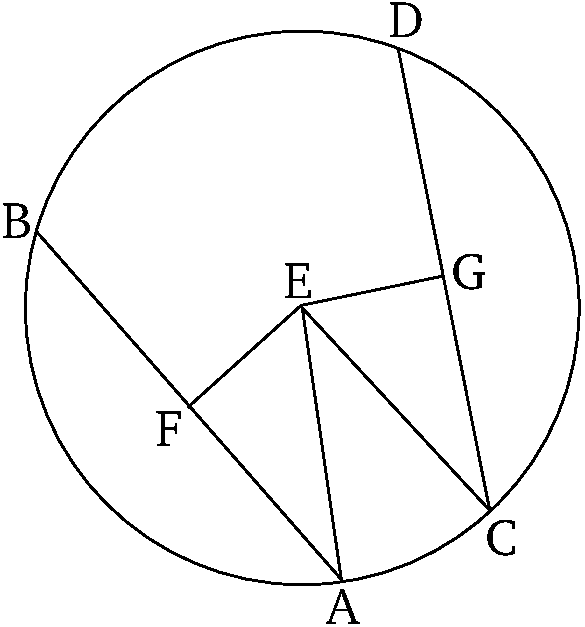
\includegraphics{Book03/fig14e.eps}}

Let $ABDC$$^{\,\dag}$ be a circle, and let $AB$ and $CD$ be equal straight-lines within it.
I say that $AB$ and $CD$ are equally far from the center.

For let the center of circle $ABDC$ be found [Prop.~3.1], and
let it be (at) $E$. And let $EF$ and $EG$ be drawn from (point) $E$, perpendicular
to $AB$ and $CD$ (respectively) [Prop.~1.12]. And let $AE$ and $EC$ be joined.

Therefore, since some straight-line, $EF$, through the center (of the circle),
cuts some (other) straight-line, $AB$, not through the center, at right-angles,
it also cuts it in half [Prop.~3.3]. Thus, $AF$ (is) equal to $FB$. Thus, 
$AB$ (is) double $AF$. So, for the same (reasons), $CD$ is also double $CG$.
And $AB$ is equal to $CD$. Thus, $AF$ (is) also equal to $CG$. And since
$AE$ is equal to $EC$, the (square) on $AE$ (is) also equal to the (square)
on $EC$. But, the (sum of the squares) on $AF$
and $EF$ (is) equal to the (square) on $AE$. For the angle at $F$ (is) a right-angle [Prop.~1.47]. And the
(sum of the squares) on $EG$ and $GC$ (is) equal to the (square) on $EC$. For the angle at $G$ (is) a right-angle [Prop.~1.47]. Thus, the (sum of the squares)
on $AF$ and $FE$ is equal to the (sum of the squares) on $CG$ and $GE$, 
of which
the (square) on $AF$ is equal to the (square) on $CG$. For $AF$ is equal to
$CG$. Thus, the remaining (square) on $FE$ is equal to the (remaining square) on  $EG$. Thus, $EF$ (is) equal to $EG$. And straight-lines in a circle are said to be equally far from the center when perpendicular (straight-lines)
which are drawn to them from the center  are equal [Def.~3.4]. Thus, $AB$ and
$CD$ are equally far from the center.

So, let the straight-lines $AB$ and $CD$ be equally far from the center. That is to say, let $EF$ be equal to $EG$. I say that $AB$ is also equal to $CD$.

For, with the same construction,  we can, similarly, show that
$AB$ is double $AF$, and $CD$ (double) $CG$. And since $AE$ is equal to $CE$, the (square) on $AE$ is equal to the (square) on $CE$. But, the (sum of the squares)
on $EF$ and $FA$ is equal to the (square) on $AE$ [Prop.~1.47]. And the (sum of
the squares) on $EG$ and $GC$ (is) equal to the (square) on $CE$ [Prop.~1.47]. Thus, the (sum of the squares) on $EF$ and $FA$ is equal to the (sum of the squares) on $EG$ and $GC$, of which the (square) on $EF$ is equal to the (square)
on $EG$. For $EF$ (is) equal to $EG$. Thus, the remaining (square) on  $AF$ is equal to the (remaining square) on  $CG$. Thus, $AF$ (is) equal to $CG$. And $AB$ is double $AF$, and
$CD$ double $CG$. Thus, $AB$ (is) equal to $CD$.

Thus, in a circle, equal straight-lines are equally far from the center, and
(straight-lines) which are equally far from the center are equal to one another.
(Which is) the very thing it was required to show.}
\end{Parallel}
{\footnotesize \noindent$^\dag$ The Greek text has ``$ABCD$'', which is obviously a
mistake.}

%%%%%%
% Prop 3.15
%%%%%%
\pdfbookmark[1]{Proposition 3.15}{pdf3.15}
\begin{Parallel}{}{} 
\ParallelLText{
\begin{center}
{\large \ggn{15}.}
\end{center}\vspace*{-7pt}

\gr{Ἐν κύκλῳ μεγίστη μὲν ἡ διάμετροξ, τῶν δὲ >άλλων ἀεὶ ἡ >έγγιον τοῦ κέντρου τῆξ ἀπώτερον μείζων ἐστίν.}

\gr{>'Εστω κύκλοξ ὁ ΑΒΓΔ, διάμετροξ δὲ α\kern -.7pt  ὐτοῦ >έστω ἡ ΑΔ, κέντρον δὲ τὸ Ε, καὶ >έγγιον μὲν τῆξ ΑΔ διαμέτρου >έστω ἡ ΒΓ, ἀπώτερον δὲ ἡ ΖΗ; λέγω, <ότι μεγίστη μέν ἐστιν ἡ ΑΔ, μείζων δὲ ἡ ΒΓ τῆξ ΖΗ.}

\gr{>'Ηθθωσαν γὰρ ἀπὸ τοῦ Ε κέντρου ἐπὶ τὰξ ΒΓ, ΖΗ κάθετοι αἱ ΕJ, ΕΚ.
καὶ ἐπεὶ >έγγιον μὲν τοῦ κέντρου ἐστὶν ἡ ΒΓ, ἀπώτερον δὲ
ἡ ΖΗ, μείζων >άρα ἡ ΕΚ τῆξ ΕJ. κείσθω τῆ| ΕJ >ίση ἡ ΕΛ,
καὶ διὰ τοῦ Λ τῆ| ΕΚ πρὸξ ὀρθὰξ ἀθθεῖσα ἡ ΛΜ διήθθω ἐπὶ
τὸ Ν, καὶ ἐπεζεύθθωσαν αἱ ΜΕ, ΕΝ, ΖΕ, ΕΗ.}

\gr{Καὶ ἐπεὶ >ίση ἐστὶν ἡ ΕJ τῆ| ΕΛ, >ίση ἐστὶ καὶ ἡ ΒΓ τῆ| ΜΝ. πάλιν, ἐπεὶ >ίση ἐστὶν ἡ μὲν ΑΕ τῆ| ΕΜ, ἡ δὲ ΕΔ τῆ| ΕΝ, ἡ >άρα
ΑΔ ταῖξ ΜΕ, ΕΝ >ίση ἐστίν. ἀλλ> αἱ μὲν ΜΕ, ΕΝ τῆξ ΜΝ μείζονέξ
εἰσιν [καὶ ἡ ΑΔ τῆξ ΜΝ μείζων ἐστίν], >ίση δὲ ἡ ΜΝ τῆ| ΒΓ;
ἡ ΑΔ >άρα τῆξ ΒΓ μείζων ἐστίν. καὶ ἐπεὶ δύο αἱ ΜΕ, ΕΝ δύο
ταῖξ ΖΕ, ΕΗ >ίσαι εἰσίν, καὶ γωνία ἡ ὑπὸ ΜΕΝ γωνίαξ τῆξ ὑπὸ
ΖΕΗ μείζων [ἐστίν], βάσιξ >άρα ἡ ΜΝ βάσεωξ τῆξ ΖΗ μείζων
ἐστίν. ἀλλὰ ἡ ΜΝ τῆ| ΒΓ ἐδείθθη >ίση [καὶ ἡ ΒΓ τῆξ ΖΗ
μείζων ἐστίν]. μεγίστη μὲν >άρα ἡ ΑΔ διάμετροξ, μείζων
δὲ ἡ ΒΓ τῆξ ΖΗ.}~\\~\\~\\~\\

\epsfysize=2.2in
\centerline{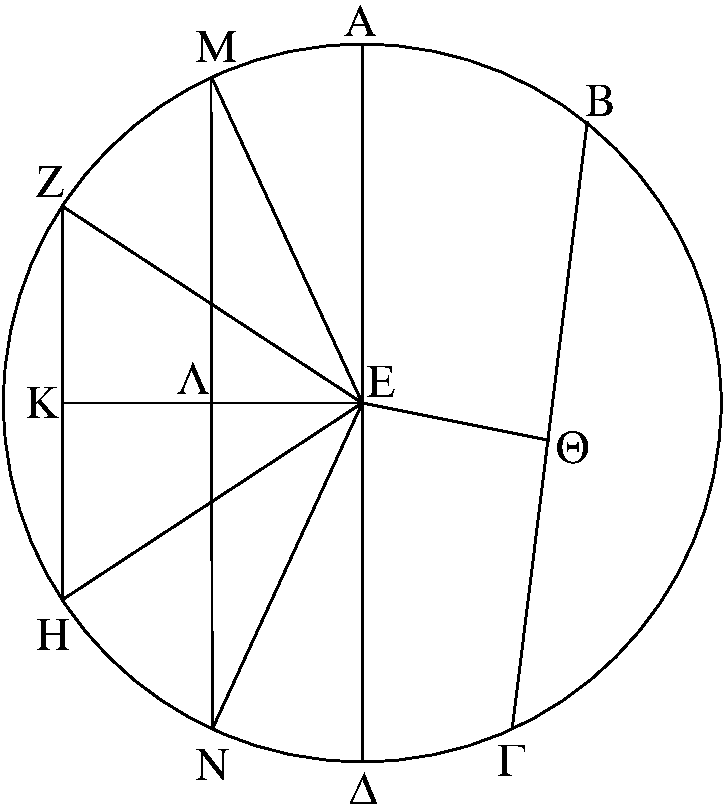
\includegraphics{Book03/fig15g.eps}}

\gr{Ἐν κύκλῳ >άρα μεγίστη μὲν έστιν ἡ διάμετροξ, τῶν δὲ >άλλων ἀεὶ ἡ >έγγιον τοῦ κέντρου τῆξ ἀπώτερον μείζων ἐστίν; <όπερ
>έδει δεῖχαι.}}

\ParallelRText{
\begin{center}
{\large Proposition 15}
\end{center}

In a circle, a diameter (is) the greatest (straight-line), and for 
the others, a (straight-line) nearer to the center is always greater than one further away.

Let $ABCD$ be a circle, and let $AD$ be its diameter, and $E$ (its) center.
And let $BC$ be nearer to the diameter $AD$,$^\dag$ and $FG$ further away. I say that
$AD$ is the greatest (straight-line), and $BC$ (is) greater than $FG$.

For let $EH$ and $EK$ be drawn from the center $E$, at right-angles
to $BC$ and $FG$ (respectively) [Prop.~1.12]. And since $BC$ is nearer to the center, and $FG$ further away, $EK$ (is) thus greater than $EH$ [Def.~3.5]. Let $EL$ be made equal to
$EH$ [Prop.~1.3]. And $LM$ being drawn through $L$, at right-angles to $EK$ [Prop.~1.11], 
let it be drawn through to $N$. And let $ME$, $EN$, $FE$, and $EG$
be joined.

And since $EH$ is equal to $EL$, $BC$ is also equal to $MN$ [Prop.~3.14]. Again,
since $AE$ is equal to $EM$, and $ED$ to $EN$, $AD$ is thus equal to $ME$ and $EN$.
But, $ME$ and $EN$ is greater than $MN$ [Prop.~1.20] [also $AD$ is greater than $MN$], and $MN$ (is) equal to $BC$. Thus, $AD$ is greater than $BC$. And since
the two (straight-lines) $ME$, $EN$ are equal to the two (straight-lines) $FE$, $EG$ (respectively),
and angle $MEN$ [is] greater than angle $FEG$,$^\ddag$ the base $MN$ is thus
greater than the base $FG$ [Prop.~1.24]. But, $MN$ was shown (to be) equal to $BC$ [(so) $BC$ is also greater than $FG$]. Thus, the diameter $AD$ (is) the
greatest (straight-line), and $BC$ (is) greater than $FG$.

\epsfysize=2.2in
\centerline{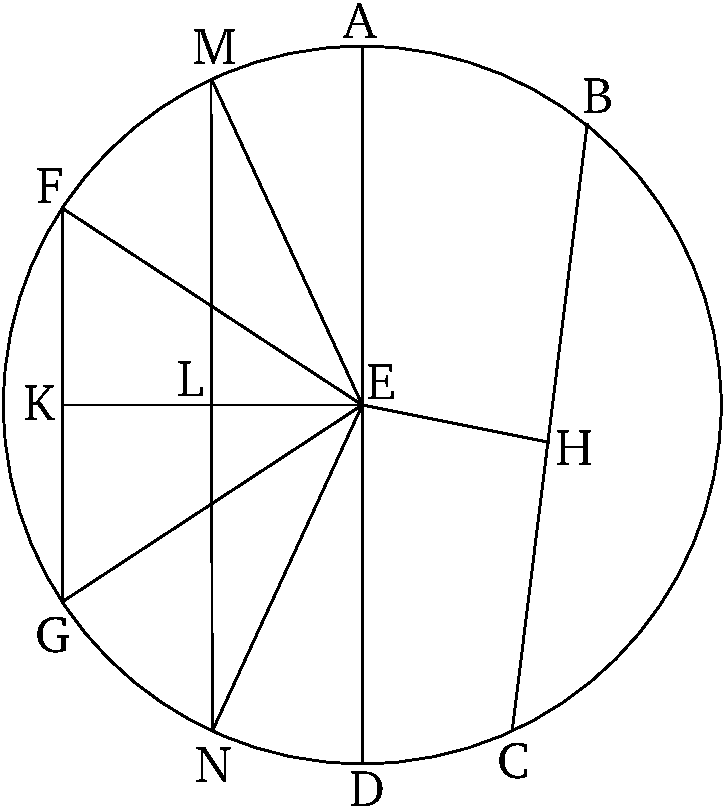
\includegraphics{Book03/fig15e.eps}}

Thus, in a circle, a diameter (is) the greatest (straight-line), and for 
the others, a (straight-line) nearer to the center is always greater than one further away. (Which is) the very thing it was required to show.}
\end{Parallel}
{\footnotesize \noindent$^\dag$ Euclid should have said ``to the center'', rather than "to the diameter $AD$", since $BC$, $AD$ and $FG$ are not necessarily parallel.\\
$^\ddag$  This is not proved,
except by reference to the figure.}

%%%%%%
% Prop 3.16
%%%%%%
\pdfbookmark[1]{Proposition 3.16}{pdf3.16}
\begin{Parallel}{}{} 
\ParallelLText{
\begin{center}
{\large \ggn{16}.}
\end{center}\vspace*{-7pt}

\gr{Ἡ τῆ| διαμέτρῳ τοῦ κύκλου πρὸξ ὀρθὰξ ἀπ> >άκραξ ἀγομένη
ἐκτὸξ πεσεῖται τοῦ κύκλου, καὶ εἰξ τὸν μεταχὺ τόπον τῆξ τε
εὐθείαξ καὶ τῆξ περιφερείαξ ἑτέρα εὐθεῖα οὐ παρεμπεσεῖται,
καὶ ἡ μὲν τοῦ ἡμικυκλίου γωνία ἁπάσηξ γωνίαξ ὀχείαξ
εὐθυγράμμου μείζων ἐστίν, ἡ δὲ λοιπὴ ἐλάττων.}

\gr{>'Εστω κύκλοξ ὁ ΑΒΓ περὶ κέντρον τὸ Δ καὶ διάμετρον τὴν
ΑΒ; λέγω, <ότι ἡ ἀπὸ τοῦ Α τῆ| ΑΒ πρὸξ ὀρθὰξ ἀπ> >άκραξ ἀγομένη ἐκτὸξ πεσεῖται τοῦ κύκλου.}

\gr{μ\kern -.7pt  ὴ γάρ, ἀλλ> εἰ δυνατόν, πιπτέτω ἐντὸξ ὡξ ἡ ΓΑ, καὶ ἐπεζεύθθω ἡ ΔΓ.}

\gr{Ἐπεὶ >ίση ἐστὶν ἡ ΔΑ τῆ| ΔΓ, >ίση ἐστὶ καὶ γωνία ἡ ὑπὸ ΔΑΓ γωνίᾳ τῆ| ὑπὸ ΑΓΔ. ὀρθὴ δὲ ἡ ὑπὸ ΔΑΓ; ὀρθὴ >άρα καὶ ἡ
ὑπὸ ΑΓΔ; τριγώνου δὴ τοῦ ΑΓΔ αἱ δύο γωνίαι αἱ ὑπὸ ΔΑΓ, ΑΓΔ
δύο ὀρθαῖξ >ίσαι εἰσίν; <όπερ ἐστὶν ἀδύνατον. οὐκ >άρα ἡ ἀπὸ
τοῦ Α σημείου τῆ| ΒΑ πρὸξ ὀρθὰξ ἀγομένη ἐντὸξ πεσεῖται
τοῦ κύκλου. ὁμοίωξ δὴ δεῖχομεν, <ότι οὐδ> ἐπὶ τῆξ περιφερείαξ;
ἐκτὸξ >άρα.}

\gr{Πιπτέτω ὡξ ἡ ΑΕ; λέγω δή, <ότι εἰξ τὸν μεταχὺ τόπον τῆξ τε ΑΕ
εὐθείαξ καὶ τῆξ ΓJΑ περιφερείαξ ἑτέρα εὐθεῖα οὐ παρεμπεσεῖται.}

\gr{Εἰ γὰρ δυνατόν, παρεμπιπτέτω ὡξ ἡ ΖΑ, καὶ >ήθθω
ἀπὸ τοῦ Δ σημείου ἐπὶ τὴν ΖΑ κάθετοξ ἡ ΔΗ. καὶ ἐπεὶ ὀρθή
ἐστιν ἡ ὑπὸ ΑΗΔ, ἐλάττων δὲ ὀρθῆξ ἡ ὑπὸ ΔΑΗ, μείζων >άρα
ἡ ΑΔ τῆξ ΔΗ. >ίση δὲ ἡ ΔΑ τῆ| ΔJ; μείζων >άρα ἡ ΔJ τῆξ
ΔΗ, ἡ ἐλάττων τῆξ μείζονοξ; <όπερ ἐστὶν ἀδύνατον. οὐκ >άρα
εἰξ τὸν μεταχὺ τόπον τῆξ τε εὐθείαξ καὶ τῆξ περιφερείαξ ἑτέρα
εὐθεῖα παρεμπεσεῖται.}\\~\\~\\~\\

\epsfysize=2in
\centerline{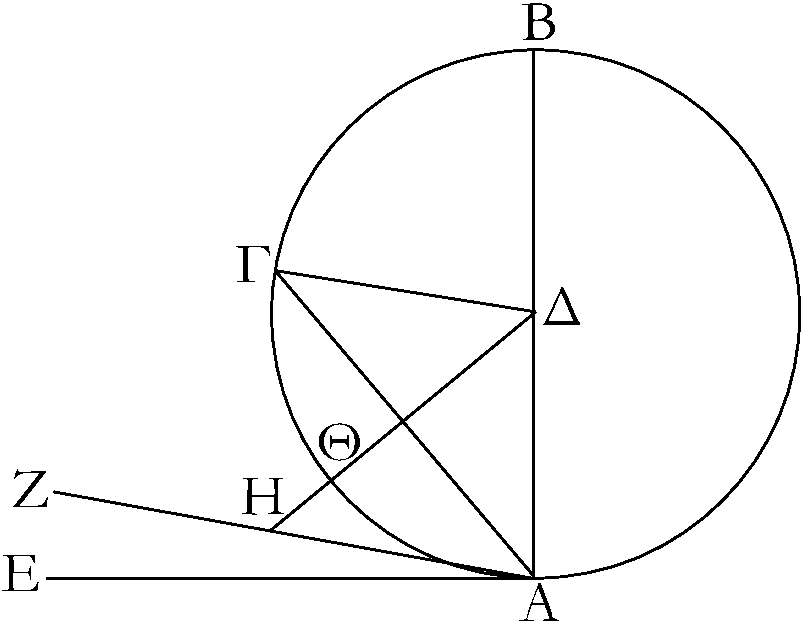
\includegraphics{Book03/fig16g.eps}}

\gr{Λέγω, <ότι καὶ ἡ μὲν τοῦ ἡμικυκλίου γωνία ἡ περιεθομένη ὑπό
τε τῆξ ΒΑ εὐθείαξ καὶ τῆξ ΓJΑ περιφερείαξ ἁπάσηξ γωνίαξ
ὀχείαξ εὐθυγράμμου μείζων ἐστίν, ἡ δὲ λοιπὴ ἡ περιεθομένη
ὑπό τε τῆξ ΓJΑ περιφερείαξ καὶ τῆξ ΑΕ εὐθείαξ ἁπάσηξ γωνίαξ
ὀχείαξ εὐθυγράμμου ἐλάττων ἐστίν.}

\gr{Εἰ γὰρ ἐστί τιξ γωνία εὐθύγραμμοξ μείζων μὲν τῆξ περιεθομένηξ
ὑπό τε τῆξ ΒΑ εὐθείαξ καὶ τῆξ ΓJΑ περιφερείαξ, ἐλάττων δὲ τῆξ
περιεθομένηξ ὑπό τε τῆξ ΓJΑ περιφερείαξ καὶ τὴξ ΑΕ εὐθείαξ, εἰξ
τὸν μεταχὺ τόπον τῆξ τε ΓJΑ περιφερείαξ καὶ τῆξ ΑΕ εὐθείαξ
εὐθεῖα παρεμπεσεῖται, <ήτιξ ποιήσει μείζονα
μὲν τῆξ περιεθομένηξ ὑπὸ τε τῆξ ΒΑ εὐθείαξ καὶ τῆξ  ΓJΑ
περιφερείαξ ὑπὸ εὐθειῶν περιεθομένην, ἐλάττονα δὲ τῆξ περιεθομένηξ ὑπό τε τῆξ ΓJΑ περιφερείαξ καὶ τῆξ ΑΕ εὐθείαξ.
οὐ παρεμπίπτει δέ; οὐκ >άρα τῆξ περιεθομένηξ γωνίαξ ὑπό
τε τῆξ ΒΑ εὐθείαξ καὶ τῆξ ΓJΑ περιφερείαξ >έσται μείζων ὀχεῖα
ὑπὸ εὐθειῶν περιεθομένη, οὐδὲ μ\kern -.7pt  ὴν ἐλάττων τῆξ περιεθομένηξ
ὑπό τε τῆξ ΓJΑ περιφερείαξ καὶ τῆξ ΑΕ εὐθείαξ.}\\~\\

\begin{center}
{\large \gr{Πόρισμα}.}
\end{center}\vspace*{-7pt}

\gr{Ἐκ δὴ τούτου φανερόν, <ότι ἡ τῆ| διαμέτρῳ τοῦ κύκλου πρὸξ
ὀρθὰξ ἀπ> >άκραξ ἀγομένη ἐφάπτεται τοῦ κύκλου [καὶ <ότι εὐθεῖα κύκλου καj> <ὲν μόνον ἐφάπτεται σημεῖον, ἐπειδήπερ καὶ ἡ κατὰ δύο
α\kern -.7pt  ὐτῶ| συμβάλλουσα ἐντὸξ α\kern -.7pt  ὐτοῦ πίπτουσα ἐδείθθη]; <όπερ
>έδει δεῖχαι.}}

\ParallelRText{
\begin{center}
{\large Proposition 16}
\end{center}

A (straight-line) drawn at right-angles to the diameter of a circle, from its
end, will fall outside the circle. And another straight-line cannot be inserted
into the space between the (aforementioned) straight-line and the circumference. And the
  angle of the semi-circle is greater than any acute rectilinear angle whatsoever, 
and the remaining (angle is) less (than any acute rectilinear angle).

Let $ABC$ be a circle around the center $D$ and the diameter $AB$. I say that
the (straight-line) drawn from $A$, at right-angles to $AB$ [Prop~1.11], from its end, will fall
outside the circle.

For (if) not (then), if possible, let it fall inside, like $CA$ (in the figure), and let
$DC$ be joined.

Since $DA$ is equal to $DC$, angle $DAC$ is also equal to angle $ACD$ [Prop.~1.5].
And $DAC$ (is) a right-angle. Thus, $ACD$ (is) also a right-angle. So, in triangle
$ACD$, the two angles $DAC$ and $ACD$ are equal to two right-angles. 
The very thing is
impossible [Prop.~1.17]. Thus, the (straight-line) drawn from point $A$,
at right-angles to $BA$, will not fall inside the circle. So, similarly, we can show 
that neither (will it fall) on the circumference. Thus, (it will fall) outside
(the circle).

Let it fall like $AE$ (in the figure). So, I say that another straight-line cannot
be inserted into the space between the straight-line $AE$ and the
circumference $CHA$.

For, if possible, let it be inserted like $FA$ (in the figure), and let $DG$ 
be drawn from point $D$, perpendicular to $FA$ [Prop.~1.12]. And since $AGD$ is a right-angle, and
 $DAG$ (is) less than a right-angle, $AD$ (is) thus greater than $DG$  [Prop.~1.19]. And $DA$ (is) equal to $DH$. Thus, $DH$ (is)
greater than $DG$, the lesser than the greater. The very thing is impossible.
Thus, another straight-line cannot be inserted into the space between the
straight-line ($AE$) and the circumference.

\epsfysize=2in
\centerline{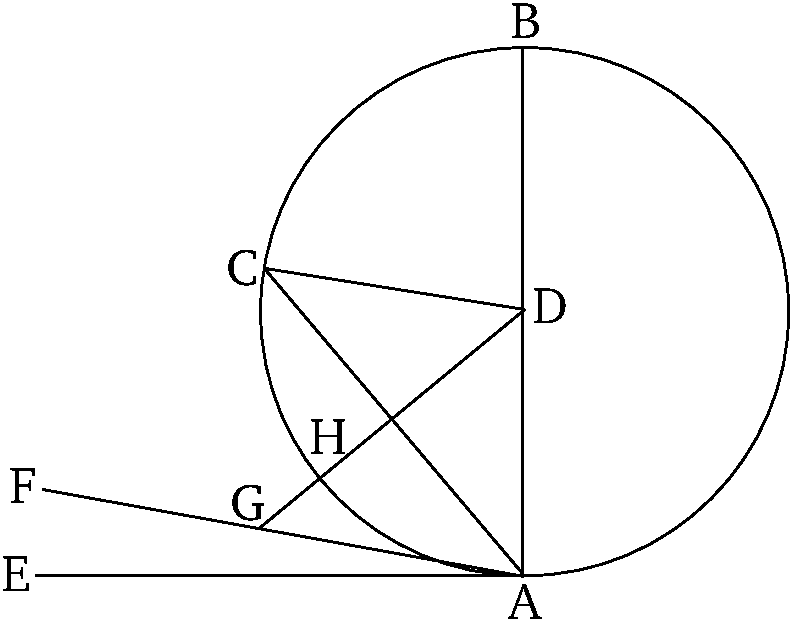
\includegraphics{Book03/fig16e.eps}}

And I also say that the  semi-circular angle  contained by the straight-line
$BA$ and the circumference $CHA$ is greater than any acute rectilinear angle whatsoever,
and the remaining (angle) contained by the circumference $CHA$ and the straight-line
$AE$ is less than any acute rectilinear angle whatsoever.

For if any rectilinear angle is greater than the (angle) contained by the
straight-line $BA$ and the circumference $CHA$, or  less than the (angle)
contained by the circumference $CHA$ and the straight-line $AE$, (then)
a straight-line can be inserted into the space between the circumference 
$CHA$ and the straight-line $AE$---anything which will make (an angle)
contained by straight-lines greater than the angle contained by the straight-line $BA$ and the circumference $CHA$, or less than the (angle) contained 
by the circumference $CHA$ and the straight-line $AE$. But (such a straight-line)
cannot be inserted. Thus, an acute (angle) contained by straight-lines
cannot be greater than the angle contained by the straight-line $BA$ and
the circumference $CHA$, neither (can it be) less than the (angle) contained by
the circumference $CHA$ and the straight-line $AE$.\\

\begin{center}
{\large Corollary}
\end{center}\vspace*{-7pt}

So, from this, (it is) manifest that a (straight-line) drawn at right-angles
to the diameter of a circle, from its extremity, touches the circle [and that the
straight-line  touches the circle at a single point, inasmuch as it was also
shown that a (straight-line) meeting (the circle) at two (points) falls inside it [Prop.~3.2]\,]. (Which is) the very thing it was required to show. }
\end{Parallel}

%%%%%%
% Prop 3.17
%%%%%%
\pdfbookmark[1]{Proposition 3.17}{pdf3.17}
\begin{Parallel}{}{} 
\ParallelLText{
\begin{center}
{\large \ggn{17}.}
\end{center}\vspace*{-7pt}

\gr{Ἀπὸ τοῦ δοθέντοξ σημείου τοῦ δοθέντοξ κύκλου ἐφαπτομένην
εὐθεῖαν γραμμ\kern -.7pt  ὴν ἀγαγεῖν.}

\gr{>'Εστω τὸ μὲν δοθὲν σημεῖον τὸ Α, ὁ δὲ δοθεὶξ κύκλοξ ὁ ΒΓΔ; δεῖ δὴ ἀπὸ τοῦ Α σημείου τοῦ ΒΓΔ κύκλου ἐφαπτομένην
εὐθεῖαν γραμμ\kern -.7pt  ὴν ἀγαγεῖν.}

\epsfysize=2.2in
\centerline{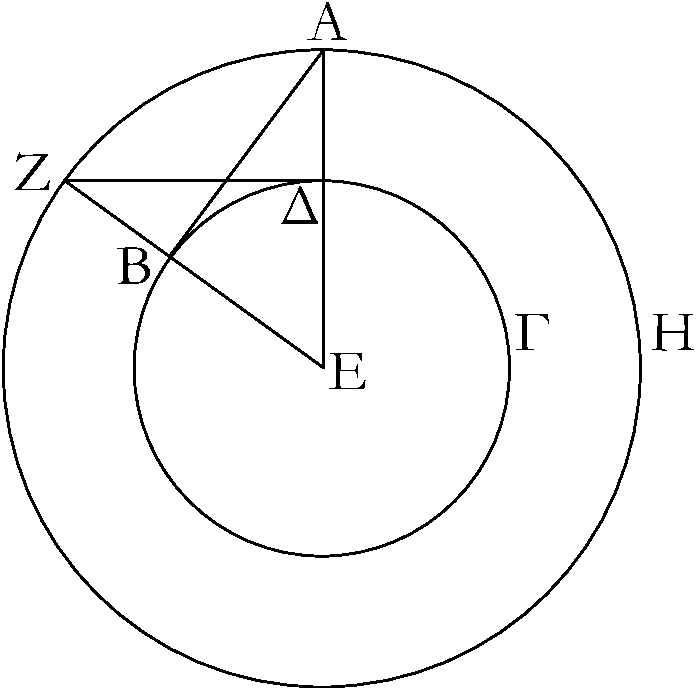
\includegraphics{Book03/fig17g.eps}}

\gr{Εἰλήφθω γὰρ τὸ κέντρον τοῦ κύκλου τὸ Ε, καὶ ἐπεζεύθθω ἡ ΑΕ,
καὶ κέντρῳ μὲν τῶ| Ε διαστήματι δὲ τῶ| ΕΑ κύκλοξ γεγράφθω ὁ ΑΖΗ,
καὶ ἀπὸ τοῦ  Δ τῆ| ΕΑ πρὸξ ὀρθὰξ >ήθθω ἡ ΔΖ, καὶ
ἐπεζεύθθωσαν αἱ ΕΖ, ΑΒ; λέγω, <ότι ἀπὸ τοῦ Α σημείου τοῦ
ΒΓΔ κύκλου ἐφαπτομένη >ῆκται ἡ ΑΒ.}

\gr{Ἐπεὶ γὰρ τὸ Ε κέντρον ἐστὶ τῶν ΒΓΔ, ΑΖΗ κύκλων, >ίση
>άρα ἐστὶν ἡ μὲν ΕΑ τῆ| ΕΖ, ἡ δὲ ΕΔ τῆ| ΕΒ; δύο δὴ αἱ ΑΕ, ΕΒ δύο ταῖξ ΖΕ, ΕΔ >ίσαι εἰσίν; καὶ γωνίαν κοινὴν περιέθουσι τὴν
πρὸξ τῶ| Ε; βάσιξ >άρα ἡ ΔΖ βάσει τῆ| ΑΒ >ίση ἐστίν, καὶ τὸ ΔΕΖ τρίγωνον τῶ| ΕΒΑ τριγώνῳ >ίσον ἐστίν, καὶ αἱ λοιπαὶ
γωνίαι ταῖξ λοιπαῖξ γωνίαιξ; >ίση >άρα ἡ ὑπὸ ΕΔΖ τῆ| ὑπὸ ΕΒΑ.
ὀρθὴ δὲ ἡ ὑπὸ ΕΔΖ; ὀρθὴ >άρα καὶ ἡ ὑπὸ ΕΒΑ. καί ἐστιν
ἡ ΕΒ ἐκ τοῦ κέντρου; ἡ δὲ τῆ| διαμέτρῳ τοῦ κύκλου πρὸξ
ὀρθὰξ ἀπ> >άκραξ ἀγομένη ἐφάπτεται τοῦ κύκλου; ἡ ΑΒ >άρα
ἐφάπτεται τοῦ ΒΓΔ κύκλου.}

\gr{Ἀπὸ τοῦ  >άρα δοθέντοξ σημείου τοῦ Α τοῦ δοθέντοξ κύκλου τοῦ ΒΓΔ ἐφαπτομένη
εὐθεῖα γραμμ\kern -.7pt  ὴ >ῆκται ἡ ΑΒ; <όπερ >έδει ποιῆσαι.}}

\ParallelRText{
\begin{center}
{\large Proposition 17}
\end{center}

To draw a straight-line touching a given circle from a given point.

Let $A$ be the given point, and $BCD$ the given circle. So it is required to draw a
straight-line touching  circle $BCD$ from point $A$.

\epsfysize=2.2in
\centerline{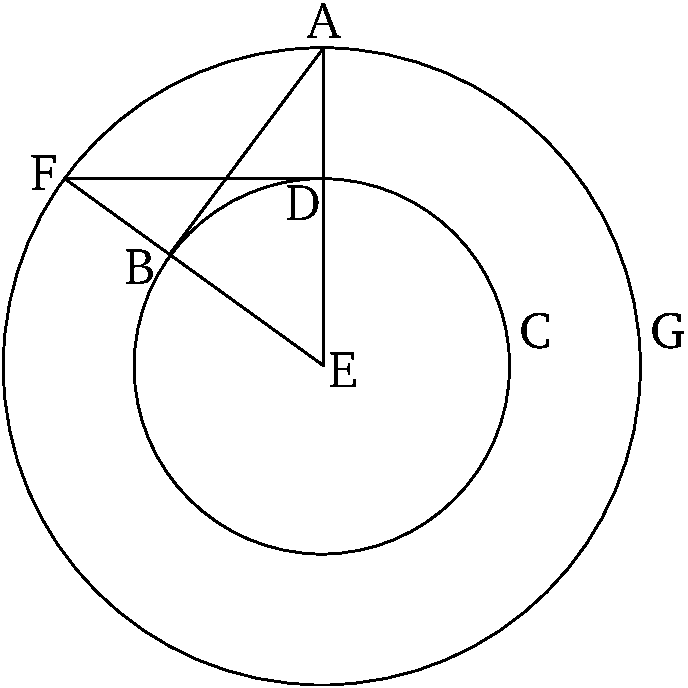
\includegraphics{Book03/fig17e.eps}}

For let the center $E$ of the circle be found [Prop.~3.1], and let $AE$ be joined. And let (the circle) $AFG$ be drawn with center
$E$ and radius $EA$. And let $DF$ be drawn from from (point) $D$,
at right-angles to $EA$ [Prop.~1.11]. And let $EF$ and $AB$ 
be  joined. I say that the (straight-line) $AB$ has been drawn from  point $A$
touching circle $BCD$.

For since $E$ is the center of circles $BCD$ and $AFG$, $EA$ is thus equal to $EF$,
and $ED$ to $EB$. So the two (straight-lines) $AE$, $EB$ are equal to
the two (straight-lines) $FE$, $ED$ (respectively). And they contain a common angle at $E$.
Thus, the base $DF$ is equal to the base $AB$, and triangle $DEF$ is equal to
triangle $EBA$, and the remaining angles (are equal) to the (corresponding)
remaining angles [Prop.~1.4]. Thus, (angle) $EDF$ (is) equal to $EBA$. And
$EDF$ (is) a right-angle. Thus, $EBA$ (is) also a right-angle. And $EB$ is a radius.
And a (straight-line) drawn at right-angles to the diameter of a circle, from
its extremity,  touches the circle [Prop.~3.16~corr.]. Thus, $AB$ touches circle $BCD$.

Thus, the straight-line $AB$ has been drawn touching the given circle $BCD$ from the given point $A$. (Which is) the very thing it was required to do.}
\end{Parallel}

%%%%%%
% Prop 3.18
%%%%%%
\pdfbookmark[1]{Proposition 3.18}{pdf3.18}
\begin{Parallel}{}{} 
\ParallelLText{
\begin{center}
{\large \ggn{18}.}
\end{center}\vspace*{-7pt}

\gr{Ἐὰν κύκλου ἐφάπτηταί τιξ εὐθεῖα, ἀπὸ δὲ τοῦ κέντρου ἐπὶ τὴν ἁφὴν ἐπιζευθθῆ| τιξ εὐθεῖα, ἡ ἐπιζευθθεῖσα κάθετοξ >έσται
ἐπὶ τὴν ἐφαπτομένην.}

\gr{Κύκλου γὰρ τοῦ ΑΒΓ ἐφαπτέσθω τιξ εὐθεῖα ἡ ΔΕ κατὰ τὸ Γ
σημεῖον, καὶ εἰλήφθω τὸ κέντρον τοῦ ΑΒΓ κύκλου τὸ
Ζ, καὶ ἀπὸ τοῦ Ζ ἐπὶ τὸ Γ ἐπεζεύθθω ἡ ΖΓ; λέγω, <ότι ἡ ΖΓ
κάθετόξ ἐστιν ἐπὶ τὴν ΔΕ.}

\gr{Εἰ γὰρ μ\kern -.7pt  ή, >ήθθω ἀπὸ τοῦ Ζ ἐπὶ τὴν ΔΕ κάθετοξ ἡ ΖΗ.}

\gr{Ἐπεὶ ο>ῦν ἡ ὑπὸ ΖΗΓ γωνία ὀρθή ἐστιν, ὀχεῖα >άρα
ἐστὶν ἡ ὑπὸ ΖΓΗ; ὑπὸ δὲ τὴν μείζονα γωνίαν ἡ μείζων
πλευρὰ ὑποτείνει; μείζων >άρα ἡ ΖΓ τῆξ ΖΗ; >ίση δὲ ἡ ΖΓ τῆ| ΖΒ;
μείζων >άρα καὶ ἡ ΖΒ τῆξ ΖΗ ἡ ἐλάττων τῆξ μείζονοξ; <όπερ
ἐστὶν ἀδύνατον. οὐκ >άρα ἡ ΖΗ κάθετόξ ἐστιν ἐπὶ τὴν ΔΕ.
ὁμοίωξ δὴ δεῖχομεν, <ότι οὐδ> >άλλη τιξ πλὴν τῆξ ΖΓ;
ἡ ΖΓ >άρα κάθετόξ ἐστιν ἐπὶ τὴν ΔΕ.}\\~\\~\\

\epsfysize=2.2in
\centerline{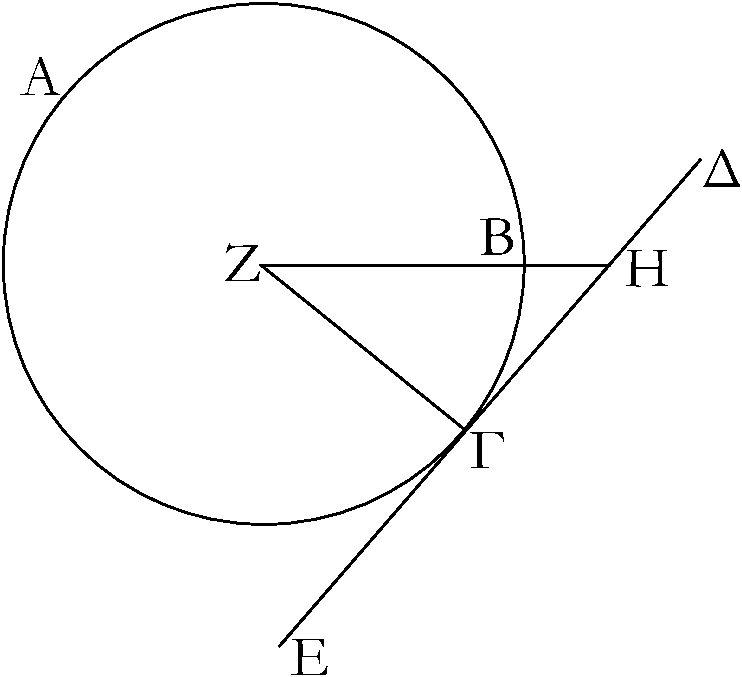
\includegraphics{Book03/fig18g.eps}}

\gr{Ἐὰν >άρα κύκλου ἐφάπτηταί τιξ εὐθεῖα, ἀπὸ δὲ τοῦ κέντρου ἐπὶ τὴν ἁφὴν ἐπιζευθθῆ| τιξ εὐθεῖα, ἡ ἐπιζευθθεῖσα κάθετοξ >έσται
ἐπὶ τὴν ἐφαπτομένην; <όπερ >έδει δεῖχαι.}}

\ParallelRText{
\begin{center}
{\large Proposition 18}
\end{center}

If some straight-line touches a circle, and some (other) straight-line is
joined from the center (of the circle) to the point of contact, (then) the (straight-line)
so joined will be perpendicular to the tangent.

For let some straight-line $DE$  touch the circle $ABC$  at  point $C$, and
let the center $F$ of circle $ABC$ be found [Prop.~3.1], 
and let $FC$ be joined from $F$ to $C$. I say that $FC$ is perpendicular
to $DE$.

For if not, let $FG$ be drawn from $F$, perpendicular to $DE$ [Prop.~1.12].

Therefore, since angle $FGC$ is a right-angle, (angle) $FCG$ is thus acute [Prop.~1.17]. And the greater angle is subtended by the greater side [Prop.~1.19]. Thus, $FC$ (is) greater than $FG$. And $FC$ (is) equal to
$FB$. Thus, $FB$ (is)  also greater than $FG$, the lesser than the greater.
The very thing is impossible. Thus, $FG$ is not perpendicular to
$DE$. So, similarly, we can show that neither (is) any other
(straight-line) except $FC$. Thus, $FC$ is perpendicular  to $DE$.

\epsfysize=2.2in
\centerline{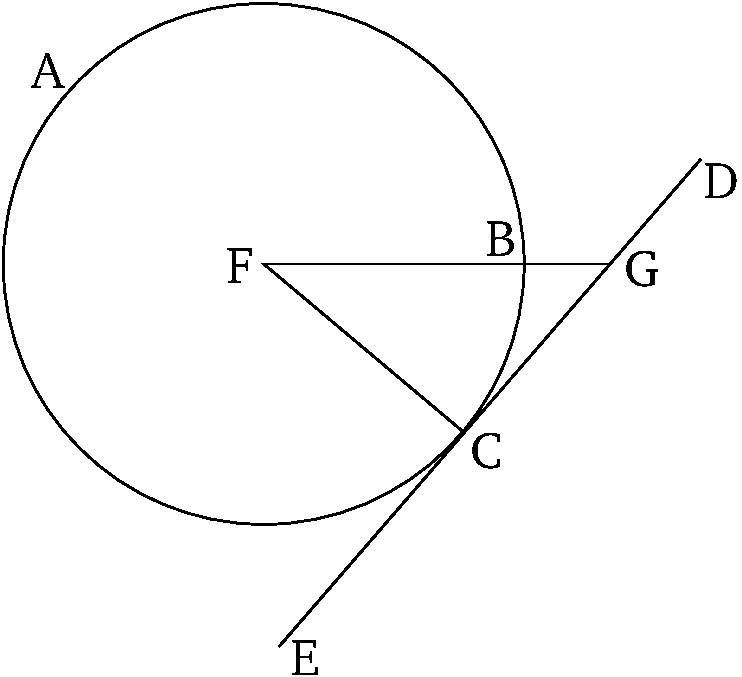
\includegraphics{Book03/fig18e.eps}}

Thus, if some straight-line  touches a circle, and some (other) straight-line is
joined from the center (of the circle) to the point of contact, (then) the (straight-line)
so joined will be perpendicular to the tangent. (Which is)
the very thing it was required to show.}
\end{Parallel}

%%%%%%
% Prop 3.19
%%%%%%
\pdfbookmark[1]{Proposition 3.19}{pdf3.19}
\begin{Parallel}{}{} 
\ParallelLText{
\begin{center}
{\large \ggn{19}.}
\end{center}\vspace*{-7pt}

\gr{Ἐὰν κύκλου ἐφάπτηταί τιξ εὐθεῖα, ἀπὸ δὲ τῆξ ἁφῆξ τῆ|
ἐφαπτομένῃ πρὸξ ὀρθὰξ [γωνίαξ] εὐθεῖα γραμμ\kern -.7pt  ὴ ἀθθῆ|,
ἐπὶ τῆξ ἀθθείσηξ >έσται τὸ κέντρον τοῦ κύκλου.}\\

\epsfysize=2.2in
\centerline{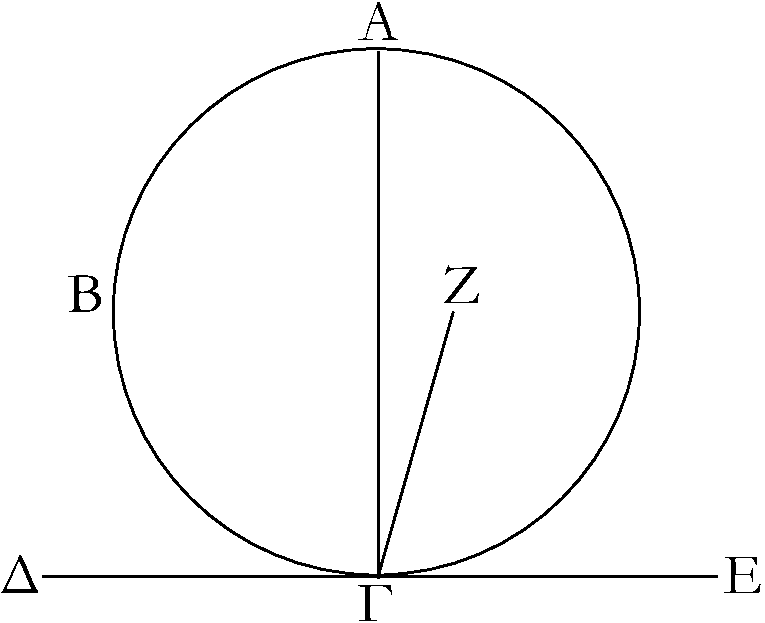
\includegraphics{Book03/fig19g.eps}}

\gr{Κύκλου γὰρ τοῦ ΑΒΓ ἐφαπτέσθω τιξ εὐθεῖα ἡ ΔΕ κατὰ τὸ Γ
σημεῖον, καὶ ἀπὸ τοῦ Γ τῆ| ΔΕ πρὸξ ὀρθὰξ >ήθθω ἡ ΓΑ;
λέγω, <ότι ἐπὶ τῆξ ΑΓ ἐστι τὸ κέντρον τοῦ κύκλου.}

\gr{μ\kern -.7pt  ὴ γάρ, ἀλλ> εἰ δυνατόν, >έστω τὸ Ζ, καὶ ἐπεζεύθθω ἡ ΓΖ.}

\gr{Ἐπεὶ [ο>ῦν] κύκλου τοῦ ΑΒΓ ἐφάπτεταί τιξ εὐθεῖα ἡ ΔΕ,
ἀπὸ δὲ τοῦ κέντρου ἐπὶ τὴν ἁφὴν ἐπέζευκται ἡ ΖΓ, ἡ ΖΓ
>άρα κάθετόξ ἐστιν ἐπὶ τὴν ΔΕ; ὀρθὴ >άρα ἐστὶν ἡ ὑπὸ ΖΓΕ. ἐστὶ
δὲ καὶ ἡ ὑπὸ ΑΓΕ ὀρθή; >ίση >άρα ἐστὶν ἡ ὑπὸ ΖΓΕ
τῆ| ὑπὸ ΑΓΕ ἡ ἐλάττων τῆ| μείζονι; <όπερ ἐστὶν ἀδύνατον.
οὐκ >άρα τὸ Ζ κέντρον ἐστὶ τοῦ ΑΒΓ κύκλου. ὁμοίωξ δὴ δείχομεν,
<ότι οὐδ> >άλλο τι πλὴν ἐπὶ τῆξ ΑΓ.}

\gr{Ἐὰν >άρα κύκλου ἐφάπτηταί τιξ εὐθεῖα, ἀπὸ δὲ τῆξ ἁφῆξ τῆ|
ἐφαπτομένῃ πρὸξ ὀρθὰξ εὐθεῖα γραμμ\kern -.7pt  ὴ ἀθθῆ|,
ἐπὶ τῆξ ἀθθείσηξ >έσται τὸ κέντρον τοῦ κύκλου; <όπερ >έδει
δεῖχαι.}}

\ParallelRText{
\begin{center}
{\large Proposition 19}
\end{center}

If some straight-line  touches a circle, and a straight-line is drawn from the
point of contact, at
right-[angles] to the tangent, (then) the center (of the circle) will be on the (straight-line) so drawn.

\epsfysize=2.2in
\centerline{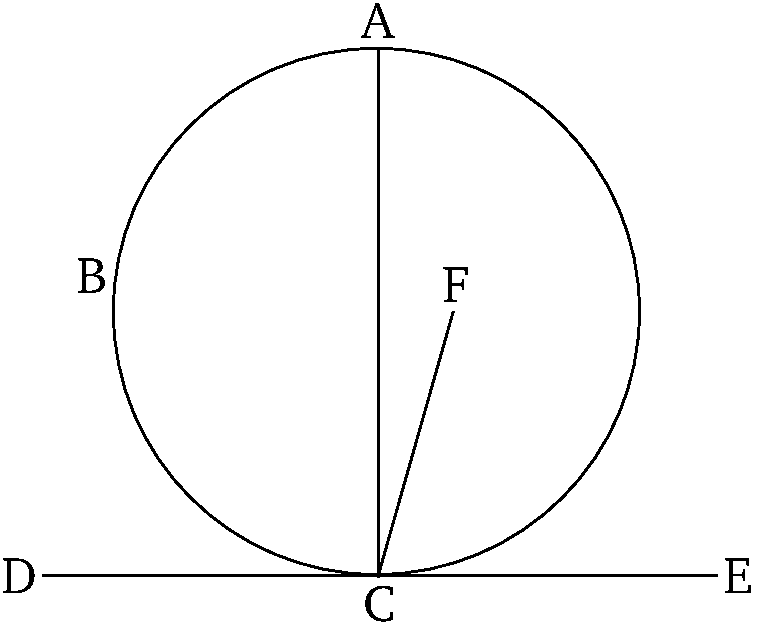
\includegraphics{Book03/fig19e.eps}}

For let some straight-line $DE$  touch the circle $ABC$  at point $C$. And let $CA$
be drawn from $C$, at right-angles to $DE$ [Prop.~1.11]. I say that the center of the circle is on $AC$.

For (if) not, if possible, let $F$ be (the center of the circle), and let
$CF$ be joined.

\mbox{[}Therefore], since some straight-line $DE$ touches the circle $ABC$, and
$FC$ has been joined from the center to the point of contact, $FC$ is thus
perpendicular to $DE$ [Prop.~3.18]. Thus, $FCE$ is a right-angle.
And $ACE$ is also a right-angle. Thus, $FCE$ is equal to $ACE$, the lesser to the
greater. The very thing is impossible. Thus, $F$ is not the center of circle $ABC$. 
So, similarly, we can show that neither is any (point) other (than one) on $AC$.

Thus, if some straight-line touches a circle, and a straight-line is drawn from the
point of contact, at
right-angles to the tangent, (then) the center (of the circle) will be on the (straight-line) so drawn. (Which is) the very thing it was required to show.}
\end{Parallel}

%%%%%%
% Prop 3.20
%%%%%%
\pdfbookmark[1]{Proposition 3.20}{pdf3.20}
\begin{Parallel}{}{} 
\ParallelLText{
\begin{center}
{\large \ggn{20}.}
\end{center}\vspace*{-7pt}

\gr{Ἐν κύκλῳ ἡ πρὸξ τῶ| κέντρῳ γωνία διπλασίων ἐστὶ τῆξ πρὸξ
τῆ| περιφερείᾳ, <όταν τὴν α\kern -.7pt  ὐτὴν περιφέρειαν βάσιν >έθωσιν αἱ
γωνίαι.}

\gr{>'Εστω κύκλοξ ὁ ΑΒΓ, καὶ πρὸξ μὲν τῶ| κέντρῳ α\kern -.7pt  ὐτοῦ γωνία
>έστω ἡ ὑπὸ ΒΕΓ, πρὸξ δὲ τῆ| περιφερείᾳ ἡ ὑπὸ ΒΑΓ, ἐθέτωσαν
δὲ τὴν α\kern -.7pt  ὐτὴν περιφέρειαν βάσιν τὴν ΒΓ; λέγω, <ότι διπλασίων ἐστὶν
ἡ ὑπὸ ΒΕΓ γωνία τῆξ ὑπὸ ΒΑΓ.}

\gr{Ἐπιζευθθεῖσα γὰρ ἡ ΑΕ διήθθω ἐπὶ τὸ Ζ.}

\gr{Ἐπεὶ ο>ῦν >ίση ἐστὶν ἡ ΕΑ τῆ| ΕΒ, >ίση καὶ γωνία
ἡ ὑπὸ ΕΑΒ τῆ| ὑπὸ ΕΒΑ; αἱ >άρα ὑπὸ ΕΑΒ, ΕΒΑ γωνίαι
τῆξ ὑπὸ ΕΑΒ διπλασίουξ εἰσίν. >ίση δὲ ἡ ὑπὸ ΒΕΖ ταῖξ
ὑπὸ ΕΑΒ, ΕΒΑ; καὶ ἡ ὑπὸ ΒΕΖ >άρα τῆξ ὑπὸ ΕΑΒ ἐστι διπλῆ. διὰ τὰ α\kern -.7pt  ὐτὰ δὴ καὶ ἡ ὑπὸ ΖΕΓ τῆξ ὑπὸ ΕΑΓ ἐστι διπλῆ. <όλη
>άρα ἡ ὑπὸ ΒΕΓ <όληξ τῆξ ὑπὸ ΒΑΓ ἐστι διπλῆ.}

\epsfysize=2.2in
\centerline{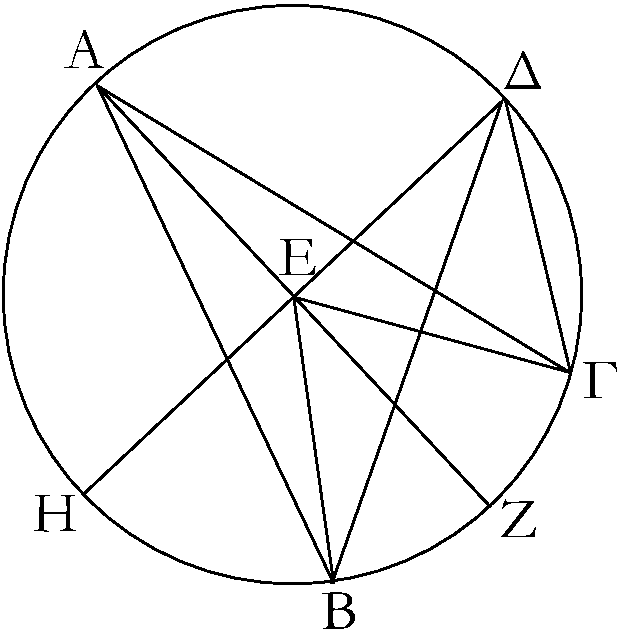
\includegraphics{Book03/fig20g.eps}}

\gr{Κεκλάσθω δὴ πάλιν, καὶ >έστω ἑτέρα γωνία ἡ ὑπὸ ΒΔΓ, καὶ
ἐπιζευθθεῖσα ἡ ΔΕ ἐκβεβλήσθω ἐπὶ τὸ Η. ὁμοίωξ
δὴ δείχομεν, <ότι διπλῆ ἐστιν ἡ ὑπὸ ΗΕΓ γωνία τῆξ ὑπὸ
ΕΔΓ, <ῶν ἡ ὑπὸ ΗΕΒ διπλῆ ἐστι τῆξ ὑπὸ ΕΔΒ; λοιπὴ
>άρα ἡ ὑπὸ ΒΕΓ διπλῆ ἐστι τῆξ ὑπὸ ΒΔΓ.}

\gr{Ἐν κύκλῳ >άρα ἡ πρὸξ τῶ| κέντρῳ γωνία διπλασίων ἐστὶ τῆξ πρὸξ
τῆ| περιφερείᾳ, <όταν τὴν α\kern -.7pt  ὐτὴν περιφέρειαν βάσιν >έθωσιν [αἱ
γωνίαι]; <όπερ >έδει δεῖχαι.}}

\ParallelRText{
\begin{center}
{\large Proposition 20}
\end{center}

In a circle, the angle at the center is double that at the circumference, when
the angles have the same circumference base.

Let $ABC$ be a circle, and let $BEC$ be an angle at its center, and $BAC$
(one) at (its) circumference. And let them have the same circumference base
$BC$. I say that angle $BEC$ is double (angle) $BAC$.

For being joined, let $AE$ be drawn through to $F$.

Therefore, since $EA$ is equal to $EB$, angle $EAB$ (is) also equal to
$EBA$ [Prop.~1.5]. Thus, angle $EAB$ and $EBA$ is double (angle) $EAB$.
And $BEF$ (is) equal to $EAB$ and $EBA$ [Prop.~1.32]. Thus, $BEF$ is also
double $EAB$. So, for the same (reasons), $FEC$ is also double $EAC$. Thus,
the whole (angle) $BEC$ is double the whole (angle) $BAC$.

\epsfysize=2.2in
\centerline{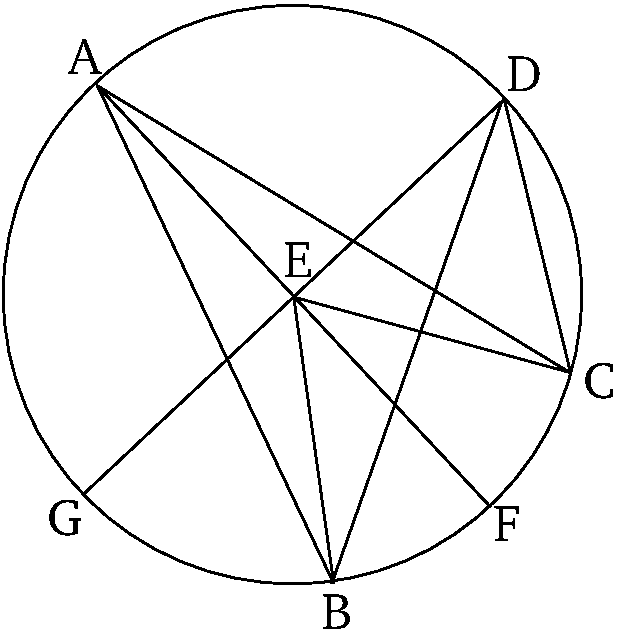
\includegraphics{Book03/fig20e.eps}}

So let another  (straight-line)  be inflected, and let there be another
angle, $BDC$. And $DE$ being joined, let it be produced to $G$.
So, similarly, we can show that angle $GEC$ is double $EDC$, of which
$GEB$ is double $EDB$. Thus, the remaining (angle) $BEC$ is double
the (remaining angle) $BDC$.

Thus, in a circle, the angle at the center is double that at the circumference, when
[the angles] have the same circumference base. (Which is) the very thing it
was required to show.\\}
\end{Parallel}

%%%%%%
% Prop 3.21
%%%%%%
\pdfbookmark[1]{Proposition 3.21}{pdf3.21}
\begin{Parallel}{}{} 
\ParallelLText{
\begin{center}
{\large \ggn{21}.}
\end{center}\vspace*{-7pt}

\gr{Ἐν κύκλῳ αἱ ἐν τῶ| α\kern -.7pt  ὐτῶ| τμ\kern -.7pt  ήματι γωνίαι >ίσαι ἀλλήλαιξ
εἰσίν.}

\epsfysize=2.2in
\centerline{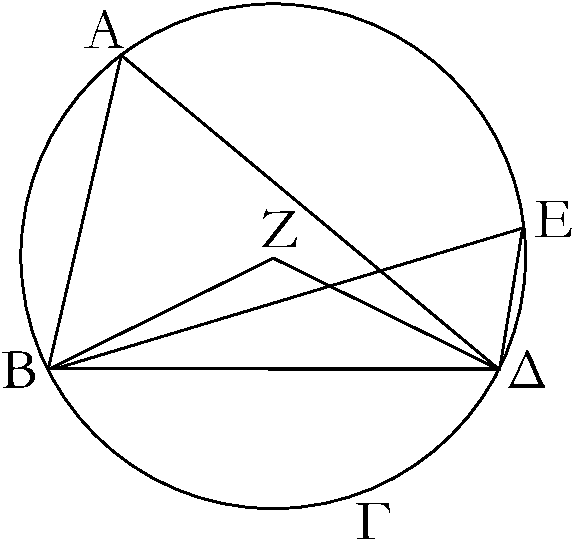
\includegraphics{Book03/fig21g.eps}}

\gr{>'Εστω κύκλοξ ὁ ΑΒΓΔ, καὶ ἐν τῶ| α\kern -.7pt  ὐτῶ| τμ\kern -.7pt  ήματι τῶ| ΒΑΕΔ γωνίαι >έστωσαν αἱ ὑπὸ ΒΑΔ, ΒΕΔ; λέγω, <ότι αἱ ὑπὸ ΒΑΔ,
ΒΕΔ γωνίαι >ίσαι ἀλλήλαιξ εἰσίν.}

\gr{Εἰλήφθω γὰρ τοῦ ΑΒΓΔ κύκλου τὸ κέντρον, καὶ >έστω τὸ Ζ, καὶ
ἐπεζεύθθωσαν αἱ ΒΖ, ΖΔ.}

\gr{Καὶ ἐπεὶ ἡ μὲν ὑπὸ ΒΖΔ γωνία πρὸξ τῶ| κέντρῳ ἐστίν,
ἡ δὲ ὑπὸ ΒΑΔ πρὸξ τῆ| περιφερείᾳ, καὶ >έθουσι τὴν α\kern -.7pt  ὐτὴν
περιφέρειαν βάσιν τὴν ΒΓΔ, ἡ >άρα ὑπὸ ΒΖΔ γωνία
διπλασίων ἐστὶ τῆξ ὑπὸ ΒΑΔ. διὰ τὰ α\kern -.7pt  ὐτὰ δὴ ἡ ὑπὸ ΒΖΔ καὶ τῆξ ὑπὸ ΒΕΔ ἐστι διπλσίων; >ίση >άρα ἡ ὑπὸ ΒΑΔ τῆ| ὑπὸ
ΒΕΔ.}

\gr{Ἐν κύκλῳ >άρα αἱ ἐν τῶ| α\kern -.7pt  ὐτῶ| τμ\kern -.7pt  ήματι γωνίαι >ίσαι ἀλλήλαιξ
εἰσίν; <όπερ >έδει δεῖχαι.}}

\ParallelRText{
\begin{center}
{\large Proposition 21}
\end{center}

In a circle, angles in the same segment are equal to one another.

\epsfysize=2.2in
\centerline{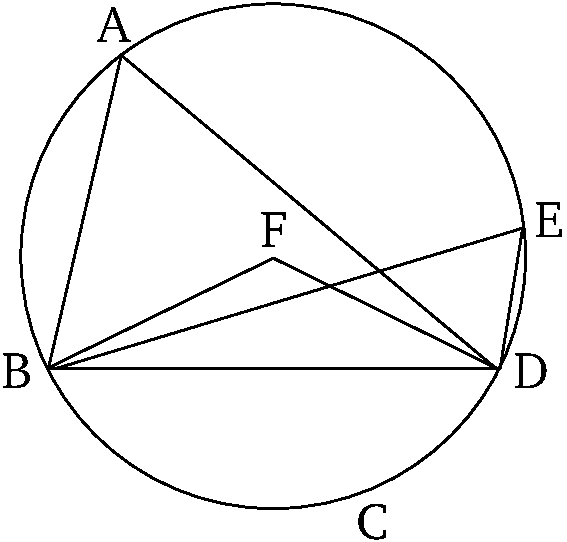
\includegraphics{Book03/fig21e.eps}}

Let $ABCD$ be a circle, and let $BAD$ and $BED$ be angles in the same segment
$BAED$. I say that angles $BAD$ and $BED$ are equal to one another.

For let the center of circle $ABCD$ be found [Prop.~3.1],
and let it be (at point) $F$. And let $BF$ and $FD$ be joined.

And since angle $BFD$ is at the center, and $BAD$ at the
circumference, and they have the same circumference base $BCD$, angle
$BFD$ is thus double $BAD$ [Prop.~3.20]. So, for the
same (reasons), $BFD$ is also double  $BED$. Thus, $BAD$ (is) equal to $BED$.

Thus, in a circle, angles in the same segment are equal to one another.
(Which is) the very thing it was required to show.}
\end{Parallel}

%%%%%%
% Prop 3.22
%%%%%%
\pdfbookmark[1]{Proposition 3.22}{pdf3.22}
\begin{Parallel}{}{} 
\ParallelLText{
\begin{center}
{\large \ggn{22}.}
\end{center}\vspace*{-7pt}

\gr{Τῶν ἐν τοῖξ κύκλοιξ τετραπλεύρων αἱ ἀπεναντίον γωνίαι δυσὶν ὀρθαῖξ >ίσαι εἰσίν.}

\epsfysize=2.2in
\centerline{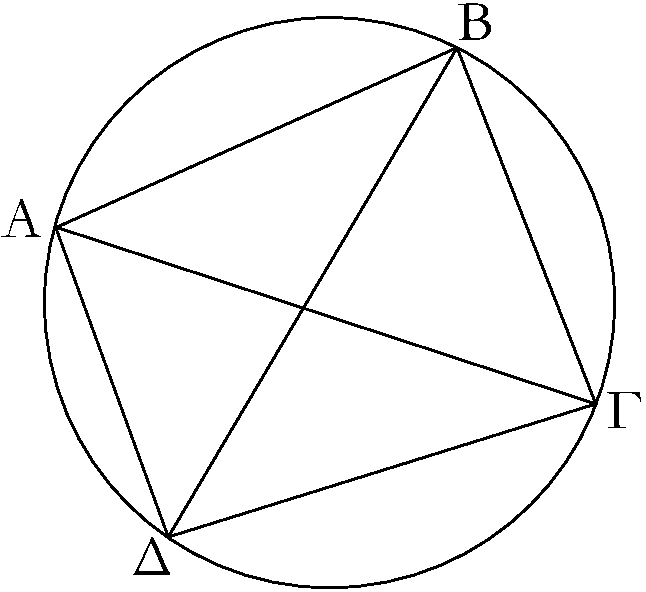
\includegraphics{Book03/fig22g.eps}}

\gr{>'Εστω κύκλοξ ὁ ΑΒΓΔ, καὶ ἐν α\kern -.7pt  ὐτῶ| τετράπλευρον >έστω τὸ ΑΒΓΔ;
λέγω, <ότι αἱ ἀπεναντίον γωνίαι δυσὶν ὀρθαῖξ >ίσαι εἰσίν.}

\gr{Ἐπεζεύθθωσαν αἱ ΑΓ, ΒΔ.}

\gr{Ἐπεὶ ο>ῦν παντὸξ τριγώνου αἱ τρεῖξ γωνίαι δυσὶν ὀρθαῖξ >ίσαι
εἰσίν, τοῦ ΑΒΓ >άρα τριγώνου αἱ τρεῖξ γωνίαι αἱ ὑπὸ ΓΑΒ, ΑΒΓ, ΒΓΑ δυσὶν ὀρθαῖξ >ίσαι εἰσίν. >ίση δὲ ἡ μὲν ὑπὸ ΓΑΒ τῆ| ὑπὸ
ΒΔΓ; ἐν γὰρ τῶ| α\kern -.7pt  ὐτῶ| τμ\kern -.7pt  ήματί εἰσι τῶ| ΒΑΔΓ; ἡ δὲ ὑπὸ ΑΓΒ
τῆ| ὑπὸ ΑΔΒ; ἐν γὰρ τῶ| α\kern -.5pt  ὐτῶ| τμ\kern -.3pt  ήματί εἰσι τῶ| ΑΔΓΒ;
<όλη >άρα ἡ ὑπὸ ΑΔΓ ταῖξ ὑπὸ ΒΑΓ, ΑΓΒ >ίση ἐστίν.
κοινὴ προσκείσθω ἡ ὑπὸ ΑΒΓ; αἱ >άρα ὑπὸ ΑΒΓ, ΒΑΓ, ΑΓΒ ταῖξ
ὑπὸ ΑΒΓ, ΑΔΓ >ίσαι εἰσίν. ἀλλ> αἱ ὑπὸ ΑΒΓ, ΒΑΓ, ΑΓΒ δυσὶν ὀρθαῖξ >ίσαι εἰσίν. καὶ αἱ ὑπὸ ΑΒΓ, ΑΔΓ >άρα δυσὶν ὀρθαῖξ
>ίσαι εἰσίν. ὁμοίωξ δὴ δείχομεν, <ότι καὶ αἱ ὑπὸ ΒΑΔ, ΔΓΒ γωνίαι δυσὶν ὀρθαῖξ >ίσαι εἰσίν.}

\gr{Τῶν >άρα ἐν τοῖξ κύκλοιξ τετραπλεύρων αἱ ἀπεναντίον γωνίαι δυσὶν ὀρθαῖξ >ίσαι εἰσίν; <όπερ >έδει δεῖχαι.}}

\ParallelRText{
\begin{center}
{\large Proposition 22}
\end{center}

For quadrilaterals within circles, the (sum of the) opposite angles is equal to two right-angles.

\epsfysize=2.2in
\centerline{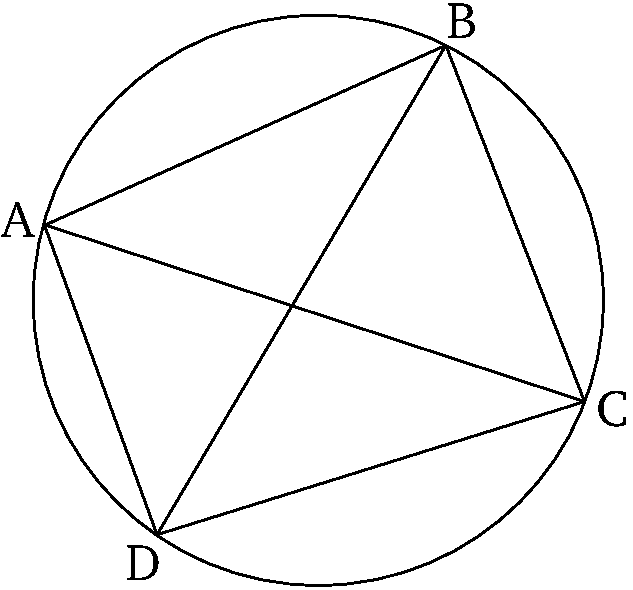
\includegraphics{Book03/fig22e.eps}}

Let $ABCD$ be a circle, and let $ABCD$ be a quadrilateral within it. I say that
the (sum of the) opposite angles is equal to two right-angles.

Let $AC$ and $BD$ be joined.

Therefore, since the three angles of any triangle are equal to two
right-angles [Prop.~1.32], the
three angles $CAB$, $ABC$, and $BCA$ of triangle $ABC$ are thus equal to two right-angles. And $CAB$ (is) equal to $BDC$. For they are in the
same segment $BADC$ [Prop.~3.21]. And $ACB$ (is equal) to $ADB$.
For they are in the same segment $ADCB$ [Prop.~3.21].
Thus, the whole of $ADC$ is equal to $BAC$ and $ACB$. Let $ABC$ be added to both. Thus, $ABC$, $BAC$, and
$ACB$ are equal to $ABC$ and $ADC$. But, $ABC$, $BAC$, and $ACB$ are equal to
two right-angles. Thus, $ABC$ and $ADC$ are also equal to two right-angles.
Similarly, we can show that angles $BAD$ and $DCB$ are also equal to
two right-angles.

Thus, for quadrilaterals within circles, the (sum of the) opposite angles is equal to two right-angles. (Which is) the very thing it was required to show.}
\end{Parallel}

%%%%%%
% Prop 3.23
%%%%%%
\pdfbookmark[1]{Proposition 3.23}{pdf3.23}
\begin{Parallel}{}{} 
\ParallelLText{
\begin{center}
{\large \ggn{23}.}
\end{center}\vspace*{-7pt}

\gr{Ἐπὶ τῆξ α\kern -.7pt  ὐτῆξ εὐθείαξ δύο τμ\kern -.7pt  ήματα κύκλων <όμοια καὶ >άνισα
οὐ συσταθήσεται ἐπὶ τὰ α\kern -.5pt  ὐτὰ μέρη.}

\gr{Εἰ γὰρ δυνατόν, ἐπὶ τῆξ α\kern -.7pt  ὐτῆξ εὐθείαξ τῆξ ΑΒ δύο τμ\kern -.7pt  ήματα
κύκλων <όμοια καὶ >άνισα συνεστάτω ἐπὶ τὰ α\kern -.5pt  ὐτὰ μέρη τὰ ΑΓΒ, ΑΔΒ,
καὶ διήθθω ἡ ΑΓΔ, καὶ ἐπεζεύθθωσαν αἱ ΓΒ, ΔΒ.}

\epsfysize=1.25in
\centerline{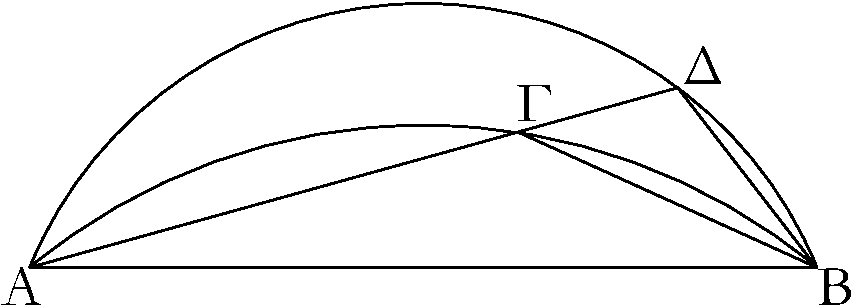
\includegraphics{Book03/fig23g.eps}}

\gr{Ἐπεὶ ο>ῦν <όμοιόν ἐστι τὸ ΑΓΒ τμ\kern -.7pt  ῆμα τῶ| ΑΔΒ τμ\kern -.7pt  ήματι,
<όμοια δὲ τμ\kern -.5pt  ήματα κύκλων ἐστὶ τὰ δεθόμενα γωνίαξ >ίσαξ, >ίση
>άρα ἐστὶν ἡ ὑπὸ ΑΓΒ γωνία τῆ| ὑπὸ ΑΔΒ ἡ ἐκτὸξ τῆ| ἐντόξ;
<όπερ ἐστὶν ἀδύνατον.}

\gr{Οὐκ >άρα ἐπὶ τῆξ α\kern -.7pt  ὐτῆξ εὐθείαξ δύο τμ\kern -.7pt  ήματα κύκλων <όμοια
καὶ >άνισα συσταθήσεται ἐπὶ τὰ α\kern -.5pt  ὐτὰ μέρη; <όπερ >έδει δεῖχαι.}}

\ParallelRText{
\begin{center}
{\large Proposition 23}
\end{center}

Two similar and unequal segments of circles cannot be constructed on the same side of the same straight-line.

For, if possible, let the two similar and unequal segments of circles, $ACB$ and
$ADB$, be constructed on the same side of the same straight-line $AB$. And let $ACD$ be drawn through (the segments), and let $CB$ and $DB$ be joined.

\epsfysize=1.25in
\centerline{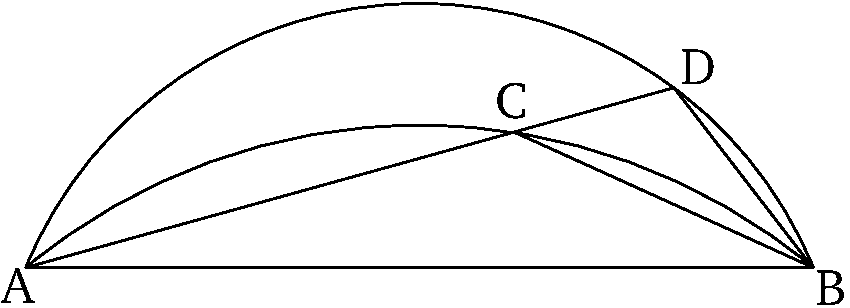
\includegraphics{Book03/fig23e.eps}}

Therefore, since segment $ACB$ is similar to segment $ADB$, and similar segments of circles are those accepting equal angles [Def.~3.11], 
angle $ACB$ is thus equal to $ADB$, the external to the internal. The very thing
is impossible [Prop.~1.16].

Thus,  two similar and unequal segments of circles cannot be constructed on the same side of the same straight-line.}
\end{Parallel}

%%%%%%
% Prop 3.24
%%%%%%
\pdfbookmark[1]{Proposition 3.24}{pdf3.24}
\begin{Parallel}{}{} 
\ParallelLText{
\begin{center}
{\large\ggn{24}.}
\end{center}\vspace*{-7pt}

\gr{Τὰ ἐπὶ >ίσων εὐθειῶν <όμοια τμ\kern -.7pt  ήματα κύλων >ίσα ἀλλήλοιξ ἐστίν.}

\gr{>'Εστωσαν γὰρ ἐπὶ >ίσων εὐθειῶν τῶν ΑΒ, ΓΔ <όμοια
τμ\kern -.7pt  ήματα κύκλων τὰ ΑΕΒ, ΓΖΔ; λέγω, <ότι >ίσον ἐστὶ τὸ ΑΕΒ
τμ\kern -.7pt  ῆμα τῶ| ΓΖΔ τμ\kern -.5pt  ήματι.}

\gr{Ἐφαρμοζομένου γὰρ τοῦ ΑΕΒ τμ\kern -.7pt  ήματοξ ἐπὶ τὸ ΓΖΔ καὶ τιθεμένου τοῦ μὲν Α σημείου ἐπὶ τὸ Γ τῆξ δὲ ΑΒ εὐθείαξ ἐπὶ τὴν
ΓΔ, ἐφαρμόσει καὶ τὸ Β σημεῖον ἐπὶ τὸ Δ σημεῖον διὰ τὸ >ίσην
ε>ῖναι τὴν ΑΒ τῆ| ΓΔ; τῆξ δὲ ΑΒ ἐπὶ τὴν ΓΔ ἐφαρμοσάσηξ ἐφαρμόσει καὶ τὸ ΑΕΒ τμ\kern -.7pt  ῆμα ἐπὶ τὸ ΓΖΔ. εἰ γὰρ ἡ ΑΒ εὐθεῖα
ἐπὶ τὴν ΓΔ ἐφαρμόσει, τὸ δὲ ΑΕΒ τμ\kern -.5pt  ῆμα ἐπὶ τὸ ΓΖΔ μ\kern -.3pt  ὴ ἐφαρμόσει, >ήτοι ἐντὸξ α\kern -.7pt  ὐτοῦ πεσεῖται >ὴ ἐκτὸξ >ὴ παραλλάχει,
ὡξ τὸ ΓΗΔ, καὶ κύκλοξ κύκλον τέμνει κατὰ πλείονα σημεῖα >ὴ
δύο; <όπερ ἐστίν ἀδύνατον. οὐκ >άρα ἐφαρμοζομένηξ τῆξ ΑΒ
εὐθείαξ ἐπὶ τὴν ΓΔ οὐκ ἐφαρμόσει καὶ τὸ ΑΕΒ τμ\kern -.7pt  ῆμα ἐπὶ
τὸ ΓΖΔ; ἐφαρμόσει >άρα, καὶ >ίσον α\kern -.7pt  ὐτῶ| >έσται.}\\~\\

\epsfysize=2.4in
\centerline{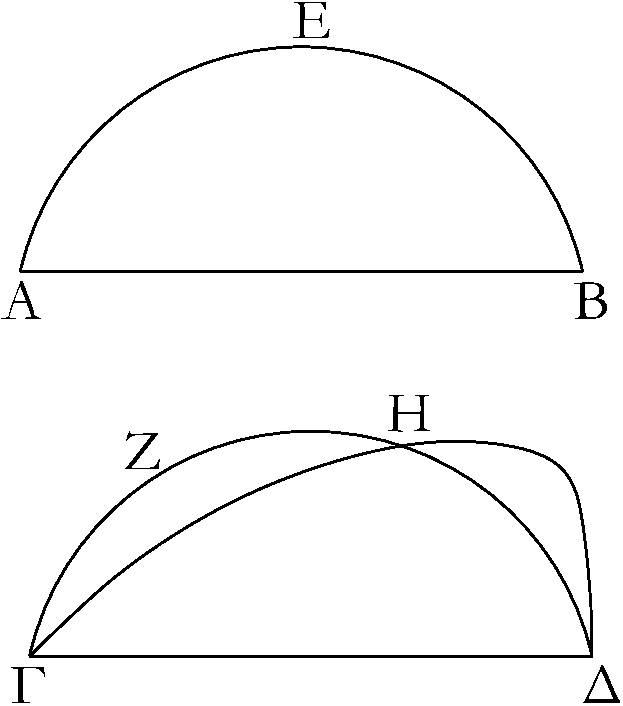
\includegraphics{Book03/fig24g.eps}}

\gr{Τὰ >άρα ἐπὶ >ίσων εὐθειῶν <όμοια τμ\kern -.7pt  ήματα κύκλων
>ίσα ἀλλήλοιξ ἐστίν; <όπερ >έδει δεῖχαι.}}

\ParallelRText{
\begin{center}
{\large Proposition 24}
\end{center}

Similar segments of circles on equal straight-lines are equal to one another.

For let $AEB$ and $CFD$ be similar segments of circles on the equal straight-lines $AB$ and $CD$ (respectively). I say that segment $AEB$ is equal to segment
$CFD$.

For if the segment $AEB$ is applied to the segment $CFD$,  and point $A$
is placed on (point) $C$, and the straight-line $AB$ on $CD$, (then) point $B$ will also coincide with point $D$, on account of $AB$ being equal to $CD$. And
if $AB$ coincides with $CD$, (then) the segment $AEB$ will also coincide with $CFD$.
For if the straight-line $AB$ coincides with $CD$, and the segment $AEB$ does not
coincide with $CFD$, (then) it will surely either fall inside it, outside (it),$^\dag$ or
it will miss like $CGD$ (in the figure), and a circle (will) cut (another) circle
at more than two points. The very thing is impossible [Prop.~3.10].
Thus, if the straight-line $AB$ is applied to $CD$, the segment $AEB$ cannot
not also coincide with $CFD$. Thus, it will coincide, and will be equal to it [C.N.~4].\\

\epsfysize=2.4in
\centerline{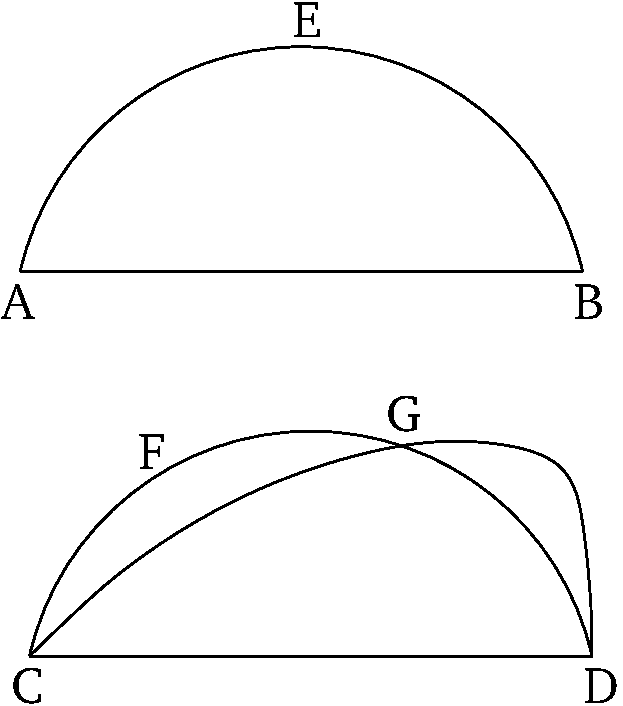
\includegraphics{Book03/fig24e.eps}}

Thus, similar segments of circles on equal straight-lines are equal to one another. (Which is) the very thing it was required to show.}
\end{Parallel}
{\footnotesize \noindent$^\dag$ Both this possibility, and the previous one, are precluded by Prop.~3.23.}

%%%%%%
% Prop 3.25
%%%%%%
\pdfbookmark[1]{Proposition 3.25}{pdf3.25}
\begin{Parallel}{}{} 
\ParallelLText{
\begin{center}
{\large \ggn{25}.}
\end{center}\vspace*{-7pt}

\gr{Κύκλου τμ\kern -.7pt  ήματοξ δοθέντοξ προσαναγράψαι τὸν κύκλον, ο<ῦπέρ ἐστι τμ\kern -.7pt  ῆμα.}

\gr{>'Εστω τὸ δοθὲν τμ\kern -.7pt  ῆμα κύκλου τὸ ΑΒΓ; δεῖ δὴ τοῦ ΑΒΓ τμ\kern -.7pt  ήματοξ
προσαναγράψαι τὸν κύκλον, ο>ῦπέρ ἐστι τμ\kern -.5pt  ῆμα.}

\gr{Τετμ\kern -.7pt  ήσθω γὰρ ἡ ΑΓ δίθα κατὰ τὸ Δ, καὶ >ήθθω ἀπὸ τοῦ Δ
σημείου τῆ| ΑΓ πρὸξ ὀρθὰξ ἡ ΔΒ, καὶ ἐπεζεύθθω ἡ ΑΒ; ἡ ὑπὸ
ΑΒΔ γωνία >άρα τῆξ ὑπὸ ΒΑΔ >ήτοι μείζων ἐστὶν >ὴ >ίση >ὴ
ἐλάττων.}

\gr{>'Εστω πρότερον μείζων, καὶ συνεστάτω πρὸξ τῆ| ΒΑ εὐθείᾳ καὶ
τῶ| πρὸξ α\kern -.7pt  ὐτῆ| σημείῳ τῶ| Α τῆ| ὑπὸ ΑΒΔ γωνίᾳ >ίση ἡ ὑπὸ
ΒΑΕ, καὶ διήθθω ἡ ΔΒ ἐπὶ τὸ Ε, καὶ ἐπεζεύθθω ἡ ΕΓ. ἐπεὶ ο>ῦν
>ίση ἐστὶν ἡ ὑπὸ ΑΒΕ γωνία τῆ| ὑπὸ ΒΑΕ, >ίση >άρα ἐστὶ
καὶ ἡ ΕΒ εὐθεῖα τῆ| ΕΑ. καὶ ἐπεὶ >ίση ἐστὶν ἡ ΑΔ τῆ|
ΔΓ, κοινὴ δὲ ἡ ΔΕ, δύο δὴ αἱ ΑΔ, ΔΕ δύο ταῖξ ΓΔ, ΔΕ >ίσαι
εἰσὶν ἑκατέρα ἑκατέρᾳ; καὶ γωνία ἡ ὑπὸ ΑΔΕ γωνίᾳ τῆ| ὑπὸ
ΓΔΕ ἐστιν >ίση; ὀρθὴ γὰρ ἑκατέρα; βάσιξ >άρα ἡ ΑΕ βάσει τῆ| ΓΕ
ἐστιν >ίση. ἀλλὰ ἡ ΑΕ τῆ| ΒΕ ἐδείθθη >ίση; καὶ ἡ ΒΕ >άρα
τῆ| ΓΕ ἐστιν >ίση; αἱ τρεῖξ >άρα αἱ ΑΕ, ΕΒ, ΕΓ >ίσαι
ἀλλήλαιξ εἰσίν; ὁ >άρα κέντρῶ| τῶ| Ε διαστήματι δὲ ἑνὶ τῶν ΑΕ, ΕΒ, ΕΓ κύκλοξ γραφόμενοξ <ήχει καὶ διὰ τῶν λοιπῶν σημείων
καὶ >έσται προσαναγεγραμμένοξ. κύκλου >άρα τμ\kern -.7pt  ήματοξ δοθέντοξ
προσαναγέγραπται ὁ κύκλοξ. καὶ δῆλον, ὡξ τὸ ΑΒΓ τμ\kern -.5pt  ῆμα >έλαττόν
ἐστιν ἡμικυκλίου διὰ τὸ τὸ Ε κέντρον ἐκτὸξ α\kern -.3pt  ὐτοῦ τυγθάνειν.}\\~\\~\\

\epsfysize=1.3in
\centerline{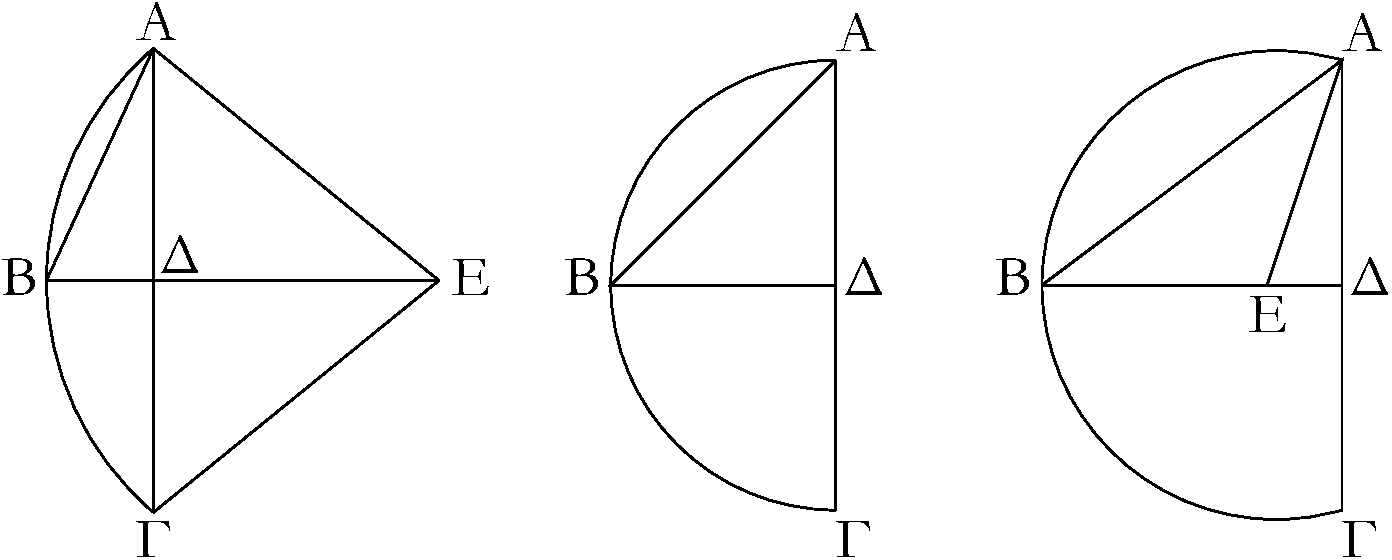
\includegraphics{Book03/fig25g.eps}}

\gr{Ὁμοίωξ [δὲ] κ>ὰν >ῆ| ἡ ὑπὸ ΑΒΔ γωνία >ίση τῆ| ὑπὸ
ΒΑΔ, τῆξ ΑΔ >ίσηξ γενομένηξ ἑκατέρᾳ τῶν ΒΔ, ΔΓ αἱ
τρεῖξ αἱ ΔΑ, ΔΒ, ΔΓ >ίσαι ἀλλήλαιξ >έσονται, καὶ >έσται τὸ Δ κέντρον
τοῦ προσαναπεπληρωμένου κύκλου, καὶ δηλαδὴ >έσται τὸ ΑΒΓ
ἡμικύκλιον.}

\gr{Ἐὰν δὲ ἡ ὑπὸ ΑΒΔ ἐλάττων >ῆ| τῆξ ὑπὸ ΒΑΔ,
καὶ συστησώμεθα πρὸξ τῆ| ΒΑ εὐθείᾳ καὶ τῶ| πρὸξ
α\kern -.7pt  ὐτῆ| σημείῳ τῶ| Α τῆ| ὑπὸ ΑΒΔ γωνίᾳ >ίσην, ἐντὸξ
τοῦ ΑΒΓ τμ\kern -.7pt  ήματοξ πεσεῖται τὸ κέντρον ἐπὶ τῆξ ΔΒ, καὶ
>έσται δηλαδὴ τὸ ΑΒΓ τμ\kern -.5pt  ῆμα μεῖζον ἡμικυκλίου.}

\gr{Κύκλου >άρα τμ\kern -.7pt  ήματοξ δοθέντοξ προσαναγέγραπται ὁ κύκλοξ;
<όπερ >έδει ποιῆσαι.}}

\ParallelRText{
\begin{center}
{\large Proposition 25}
\end{center}

For a given segment of a circle, to complete the circle, the very one of which it is a segment.

Let $ABC$ be the given segment of a circle. So it is required
to complete the circle for segment $ABC$, the very one of which it is a segment.

For let $AC$ be cut in half at (point) $D$ [Prop.~1.10], and let $DB$ be drawn
from point $D$, at right-angles to $AC$ [Prop.~1.11]. And let $AB$ be joined.
Thus, angle $ABD$ is surely either greater than,  equal to, or less than (angle)
$BAD$.

First of all, let it be greater. And let (angle) $BAE$, equal to
angle $ABD$, be constructed on the straight-line $BA$, at the point $A$ on it [Prop.~1.23].
And let $DB$ be drawn through to $E$, and let $EC$ be joined.
Therefore, since angle $ABE$ is equal to $BAE$, the straight-line $EB$ is thus also
equal to $EA$ [Prop.~1.6]. And since $AD$ is equal to $DC$, and $DE$ (is)
common, the two (straight-lines) $AD$, $DE$ are equal to the two (straight-lines)
$CD$, $DE$, respectively. And angle $ADE$ is equal to angle $CDE$. For each (is)
a right-angle. Thus, the base $AE$ is equal to the base $CE$ [Prop.~1.4].
But, $AE$ was shown (to be) equal to $BE$. Thus, $BE$ is also equal
to $CE$. Thus, the three (straight-lines) $AE$, $EB$, and $EC$ are equal to
one another. Thus, if a circle is drawn with center $E$, and radius one of $AE$, $EB$, or $EC$,  it will also go through the remaining points (of the segment), and the (associated circle) will be
 completed [Prop.~3.9]. Thus, a circle has been completed from the given
 segment of a circle. And (it is) clear that the segment $ABC$ is less
 than a semi-circle, because the center $E$ happens to lie outside it.

\epsfysize=1.3in
\centerline{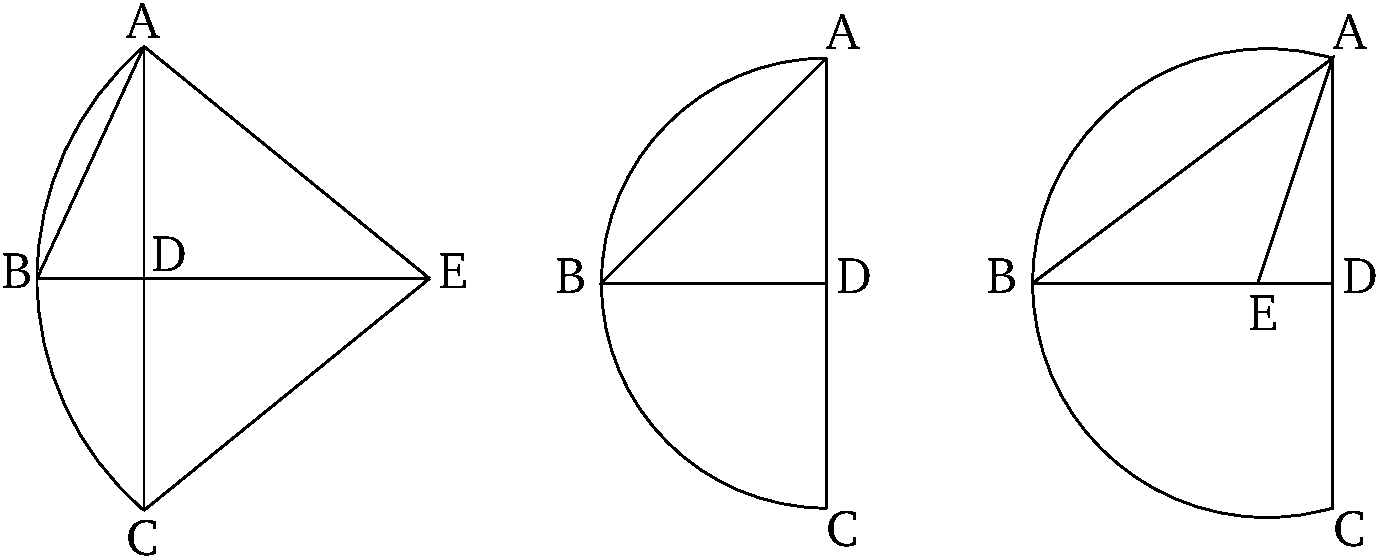
\includegraphics{Book03/fig25e.eps}}
 
\mbox{[}And], similarly, even if angle $ABD$ is equal to $BAD$,  (since) $AD$ becomes equal to
 each of $BD$ [Prop.~1.6] and $DC$, the three (straight-lines) $DA$, $DB$, and $DC$
 will  be equal to one another. And point $D$ will be the center of the completed
 circle. And $ABC$ will manifestly be a semi-circle.
 
 And if $ABD$ is less than $BAD$, and we construct (angle $BAE$), equal to angle
 $ABD$,  on the straight-line $BA$, at the point $A$ on it [Prop.~1.23], then
 the center will fall on $DB$,  inside the segment $ABC$. And segment
 $ABC$ will manifestly be greater than a semi-circle.
 
 Thus, a circle has been completed from the given segment of a circle. (Which is) the very thing it was required to do.}
\end{Parallel}

%%%%%%
% Prop 3.26
%%%%%%
\pdfbookmark[1]{Proposition 3.26}{pdf3.26}
\begin{Parallel}{}{} 
\ParallelLText{
\begin{center}
{\large \ggn{26}.}
\end{center}\vspace*{-7pt}

\gr{Ἐν τοῖξ >ίσοιξ κύκλοιξ αἱ >ίσαι γωνίαι ἐπὶ >ίσων περιφερειῶν βεβήκασιν, ἔαν τε πρὸξ τοῖξ κέντροιξ ἔαν τε πρὸξ ταῖξ περιφερείαιξ
>ῶσι βεβηκυῖαι.}

\gr{>'Εστωσαν >ίσοι κύκλοι οἱ ΑΒΓ, ΔΕΖ καὶ ἐν α\kern -.7pt  ὐτοῖξ >ίσαι γωνίαι >έστωσαν πρὸξ μὲν τοῖξ κέντροιξ αἱ ὑπὸ ΒΗΓ, ΕJΖ, πρὸξ δὲ ταῖξ
περιφερείαιξ αἱ ὑπὸ ΒΑΓ, ΕΔΖ; λέγω, <ότι >ίση ἐστὶν ἡ ΒΚΓ
περιφέρεια τῆ| ΕΛΖ περιφερείᾳ.}

\gr{Ἐπεζεύθθωσαν γὰρ αἱ ΒΓ, ΕΖ.}

\gr{Καὶ ἐπεὶ >ίσοι εἰσὶν οἱ ΑΒΓ, ΔΕΖ κύκλοι, >ίσαι
εἰσὶν αἱ ἐκ τῶν κέντρων; δύο δὴ αἱ ΒΗ, ΗΓ
δύο ταῖξ ΕJ, JΖ >ίσαι; καὶ γωνία ἡ πρὸξ τῶ| Η γωνίᾳ τῆ| πρὸξ
τῶ| J >ίση; βάσιξ >άρα ἡ ΒΓ βάσει τῆ| ΕΖ ἐστιν >ίση. καὶ ἐπεὶ
>ίση ἐστὶν ἡ πρὸξ τῶ| Α γωνία τῆ| πρὸξ τῶ| Δ, <όμοιον >άρα ἐστὶ τὸ ΒΑΓ τμ\kern -.7pt  ῆμα τῶ| ΕΔΖ τμ\kern -.7pt  ήματι; καί εἰσιν ἐπὶ >ίσων εὐθειῶν [τῶν ΒΓ, ΕΖ]; τὰ δὲ ἐπὶ >ίσων εὐθειῶν <όμοια
τμ\kern -.5pt  ήματα κύκλων >ίσα ἀλλήλοιξ ἐστίν; >ίσον >άρα τὸ ΒΑΓ τμ\kern -.3pt  ῆμα τῶ|
ΕΔΖ. >έστι δὲ καὶ <όλοξ ὁ ΑΒΓ κύκλοξ <όλῳ τῶ| ΔΕΖ κύκλῳ
>ίσοξ; λοιπὴ >άρα ἡ ΒΚΓ περιφέρεια τῆ| ΕΛΖ περιφερείᾳ ἐστὶν >ίση.}\\~\\~\\

\epsfysize=1.5in
\centerline{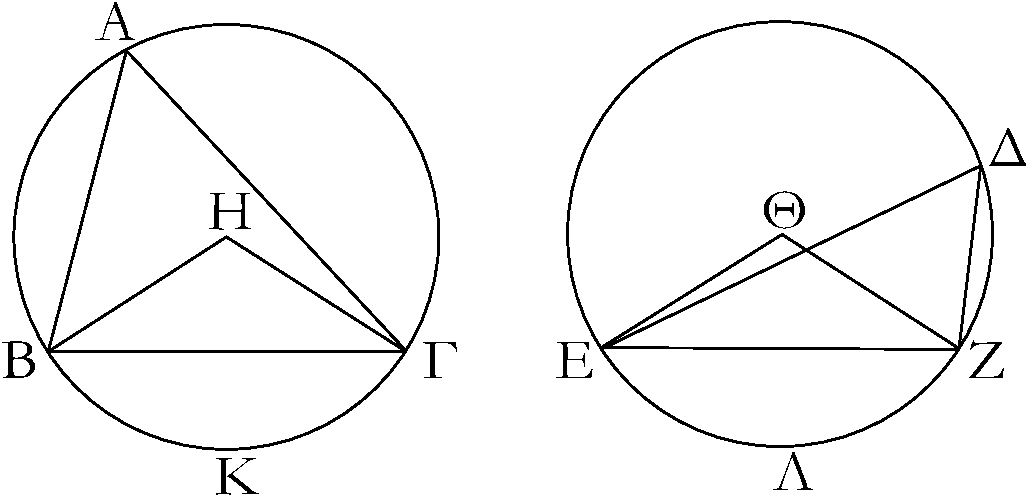
\includegraphics{Book03/fig26g.eps}}

\gr{Ἐν >άρα τοῖξ >ίσοιξ κύκλοιξ αἱ >ίσαι γωνίαι ἐπὶ >ίσων
περιφερειῶν βεβήκασιν, ἔαν τε πρὸξ τοῖξ κέντροιξ ἔαν
τε πρὸξ ταῖξ περιφερείαξ >ῶσι βεβηκυῖαι; <όπερ >έδει
δεῖχαι.}}

\ParallelRText{
\begin{center}
{\large Proposition 26}
\end{center}

In equal circles, equal angles stand upon equal circumferences  whether they
are standing at the center or at the circumference.

Let $ABC$ and $DEF$ be equal circles, and within them let $BGC$ and $EHF$ be equal angles at the center, and $BAC$ and $EDF$ (equal angles) at the circumference. I say that circumference $BKC$ is equal to circumference $ELF$.

For let $BC$ and $EF$ be joined.

And since circles $ABC$ and $DEF$ are equal, their radii are equal.
So the two (straight-lines) $BG$, $GC$ (are) equal to the two (straight-lines)
$EH$, $HF$ (respectively). And the angle at $G$ (is) equal to the angle at $H$.
Thus, the base $BC$ is equal to the base $EF$ [Prop.~1.4].
And since the angle at $A$ is equal to the (angle) at $D$, the segment $BAC$ is
thus similar to the segment $EDF$ [Def.~3.11]. And they are on
equal straight-lines [$BC$ and $EF$]. And similar segments of circles on equal
straight-lines are equal to one another [Prop.~3.24]. Thus, segment
$BAC$ is equal to (segment) $EDF$. And the whole circle $ABC$ is also
equal to the whole circle $DEF$. Thus, the remaining circumference $BKC$
is equal to the (remaining) circumference $ELF$.

\epsfysize=1.5in
\centerline{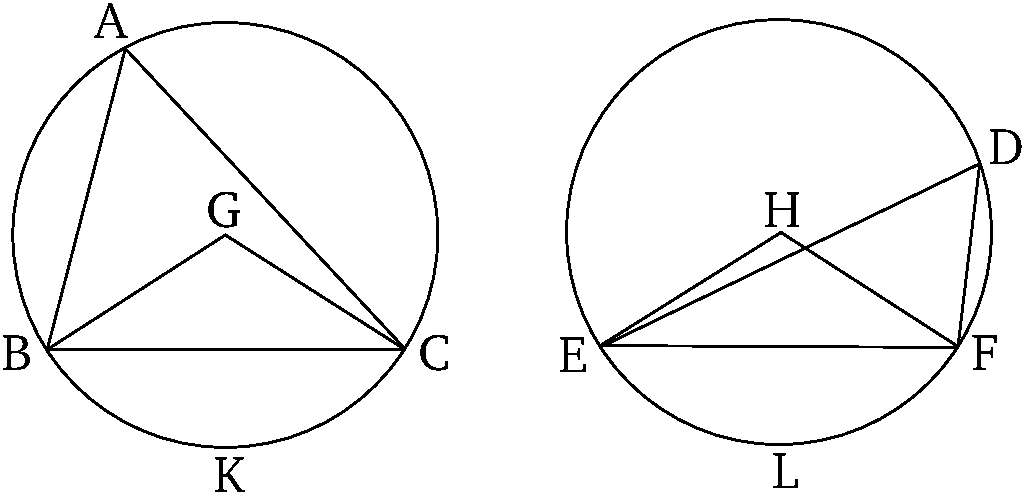
\includegraphics{Book03/fig26e.eps}}

Thus,   in equal circles, equal angles stand upon equal circumferences, whether they
are standing  at the center or at the circumference. (Which is)
the very thing which it was required to show.}
\end{Parallel}

%%%%%%
% Prop 3.27
%%%%%%
\pdfbookmark[1]{Proposition 3.27}{pdf3.27}
\begin{Parallel}{}{} 
\ParallelLText{
\begin{center}
{\large\ggn{27}.}
\end{center}\vspace*{-7pt}

\gr{Ἐν τοῖξ >ίσοιξ κύκλοιξ αἱ ἐπὶ >ίσων περιφερειῶν βεβηκυῖαι γωνίαι
>ίσαι ἀλλήλαιξ εἰσίν, ἔαν τε πρὸξ τοῖξ κέντροιξ ἔαν τε πρὸξ
ταῖξ περιφερείαιξ >ῶσι βεβηκυῖαι.}

\epsfysize=1.5in
\centerline{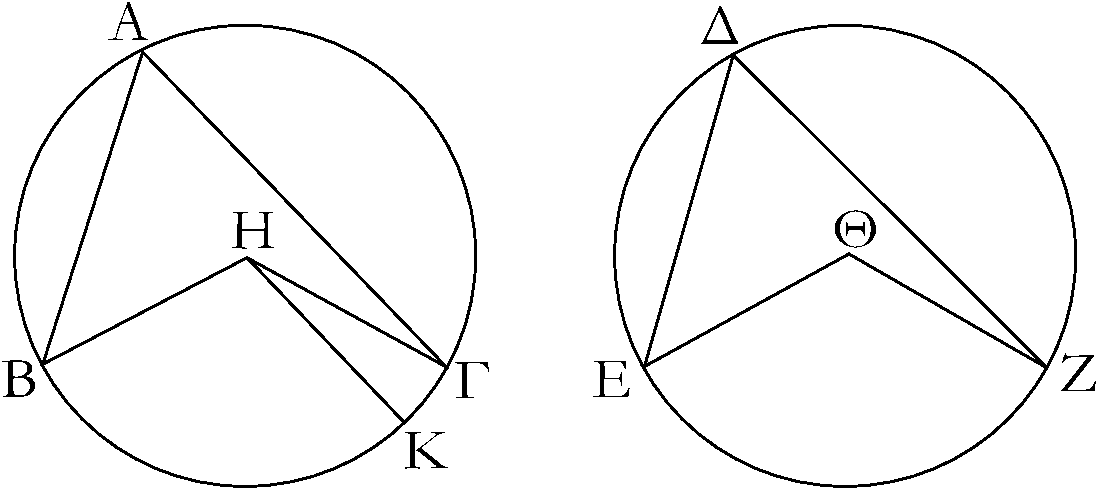
\includegraphics{Book03/fig27g.eps}}

\gr{Ἐν γὰρ >ίσοιξ κύκλοιξ τοῖξ ΑΒΓ, ΔΕΖ ἐπὶ >ίσων περιφερειῶν
τῶν ΒΓ, ΕΖ πρὸξ μὲν τοῖξ Η, J κέντροιξ γωνίαι βεβηκέτωσαν αἱ
ὑπὸ ΒΗΓ, ΕJΖ, πρὸξ δὲ ταῖξ περιφερείαιξ αἱ ὑπὸ ΒΑΓ, ΕΔΖ;
λέγω, <ότι ἡ μὲν ὑπὸ ΒΗΓ γωνία τῆ| ὑπὸ ΕJΖ ἐστιν >ίση,
ἡ δὲ ὑπὸ ΒΑΓ τῆ| ὑπὸ ΕΔΖ ἐστιν >ίση.}

\gr{Εἰ γὰρ >άνισόξ ἐστιν ἡ ὑπὸ ΒΗΓ τῆ| ὑπὸ ΕJΖ,
μία α\kern -.7pt  ὐτῶν μείζων ἐστίν. >έστω μείζων ἡ ὑπὸ ΒΗΓ, καὶ
συνεστάτω πρὸξ τῆ| ΒΗ εὐθείᾳ καὶ τῶ| πρὸξ α\kern -.7pt  ὐτῆ| σημείῳ
τῶ| Η τῆ| ὑπὸ ΕJΖ γωνίᾳ >ίση ἡ ὑπὸ ΒΗΚ; αἱ δὲ >ίσαι
γωνίαι ἐπὶ >ίσων περιφερειῶν βεβήκασιν, <όταν πρὸξ τοῖξ κέντροιξ
>ῶσιν; >ίση >άρα ἡ ΒΚ περιφέρεια τῆ| ΕΖ περιφερείᾳ. ἀλλὰ ἡ ΕΖ τῆ|
ΒΓ ἐστιν >ίση; καὶ ἡ ΒΚ >άρα τῆ| ΒΓ ἐστιν >ίση ἡ ἐλάττων τῆ|
μείζονι; <όπερ ἐστὶν ἀδύνατον. οὐκ >άρα >άνισόξ ἐστιν ἡ ὑπὸ
ΒΗΓ γωνία τῆ| ὑπὸ ΕJΖ; >ίση >άρα. καί ἐστι τῆξ μὲν ὑπὸ ΒΗΓ
ἡμίσεια ἡ πρὸξ τῶ| Α, τῆξ δὲ ὑπὸ  ΕJΖ ἡμίσεια
ἡ πρὸξ τῶ| Δ; >ίση >άρα καὶ ἡ πρὸξ τῶ| Α γωνία τῆ| πρὸξ
τῶ| Δ.}

\gr{Ἐν >άρα τοῖξ >ίσοιξ κύκλοιξ αἱ ἐπὶ >ίσων περιφερειῶν βεβηκυῖαι
γωνίαι >ίσαι ἀλλήλαιξ εἰσίν, ἔαν τε πρὸξ τοῖξ κέντροιξ ἔαν
τε πρὸξ ταῖξ περιφερείαιξ >ῶσι βεβηκυῖαι; <όπερ >έδει δεῖχαι.}}

\ParallelRText{
\begin{center}
{\large Proposition 27}
\end{center}

In equal circles, angles standing upon equal circumferences  are equal to one
another, whether they are standing at the center or at the circumference.

\epsfysize=1.5in
\centerline{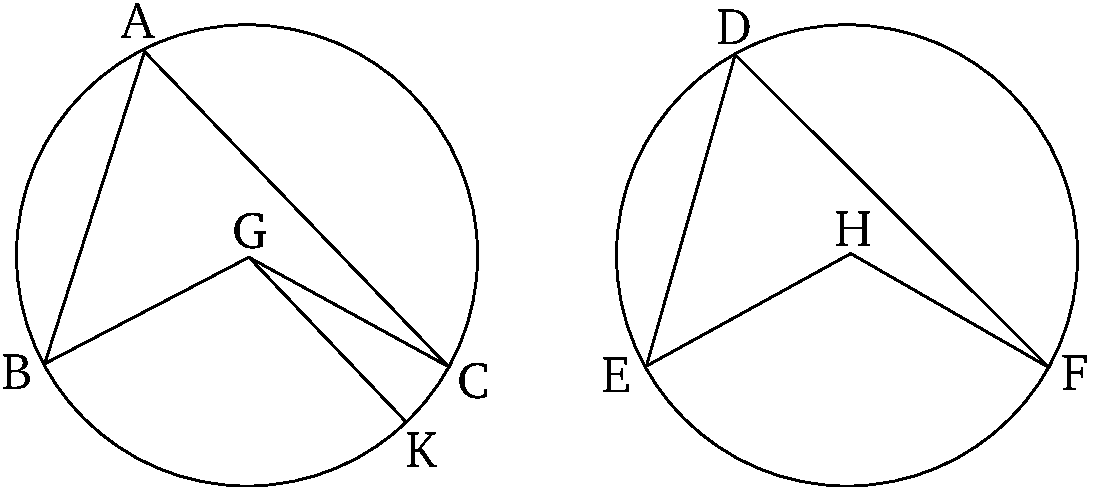
\includegraphics{Book03/fig27e.eps}}

For let the angles $BGC$ and $EHF$ at the centers $G$ and $H$, and the (angles) $BAC$ and $EDF$
at the circumferences, stand upon the equal circumferences $BC$ and $EF$, in the equal circles $ABC$ and $DEF$ (respectively). I say that angle $BGC$ is
equal to (angle) $EHF$, and $BAC$ is equal to $EDF$.

For if $BGC$ is unequal to $EHF$, one of them is greater. Let $BGC$ be greater, 
and let the (angle) $BGK$, equal to  angle $EHF$, be constructed on the
straight-line $BG$, at the point $G$ on it [Prop.~1.23]. But equal angles (in equal circles) stand upon equal circumferences, when they are at the centers [Prop.~3.26]. Thus,
circumference $BK$ (is) equal to circumference $EF$. But, $EF$ is equal to $BC$.
Thus, $BK$ is also equal to $BC$, the lesser to the greater. The very thing is
impossible. Thus, angle $BGC$ is not unequal to $EHF$. Thus, (it is) equal.
And the (angle) at $A$ is half $BGC$, and the (angle) at $D$ half $EHF$ [Prop.~3.20]. Thus, the angle at $A$ (is) also equal to the (angle) at $D$.

Thus, in equal circles, angles standing upon equal circumferences  are equal to one
another, whether they are standing at the center or at the circumference.
(Which is) the very thing it was required to show.\\}
\end{Parallel}

%%%%%%
% Prop 3.28
%%%%%%
\pdfbookmark[1]{Proposition 3.28}{pdf3.28}
\begin{Parallel}{}{} 
\ParallelLText{
\begin{center}
{\large\ggn{28}.}
\end{center}\vspace*{-7pt}

\gr{Ἐν τοῖξ >ίσοιξ κύκλοιξ αἱ >ίσαι εὐθεῖαι >ίσαξ περιφερείαξ ἀφαιροῦσι
τὴν μὲν μείζονα  τῆ| μείζονι τὴν δὲ ἐλάττονα τῆ| ἐλάττονι.}

\gr{>'Εστωσαν >ίσοι κύκλοι οἱ ΑΒΓ, ΔΕΖ, καὶ ἐν τοῖξ κύκλοιξ >ίσαι
εὐθεῖαι >έστωσαν αἱ ΑΒ, ΔΕ τὰξ μὲν ΑΓΒ, ΑΖΕ περιφερείαξ μείζοναξ
ἀφαιροῦσαι τὰξ δὲ ΑΗΒ, ΔJΕ ἐλάττοναξ; λέγω, <ότι ἡ μὲν ΑΓΒ
μείζων περιφέρεια >ίση ἐστὶ τῆ| ΔΖΕ μείζονι περιφερείᾳ
ἡ δὲ ΑΗΒ ἐλάττων περιφέρεια τῆ| ΔJΕ.}\\

\epsfysize=1.6in
\centerline{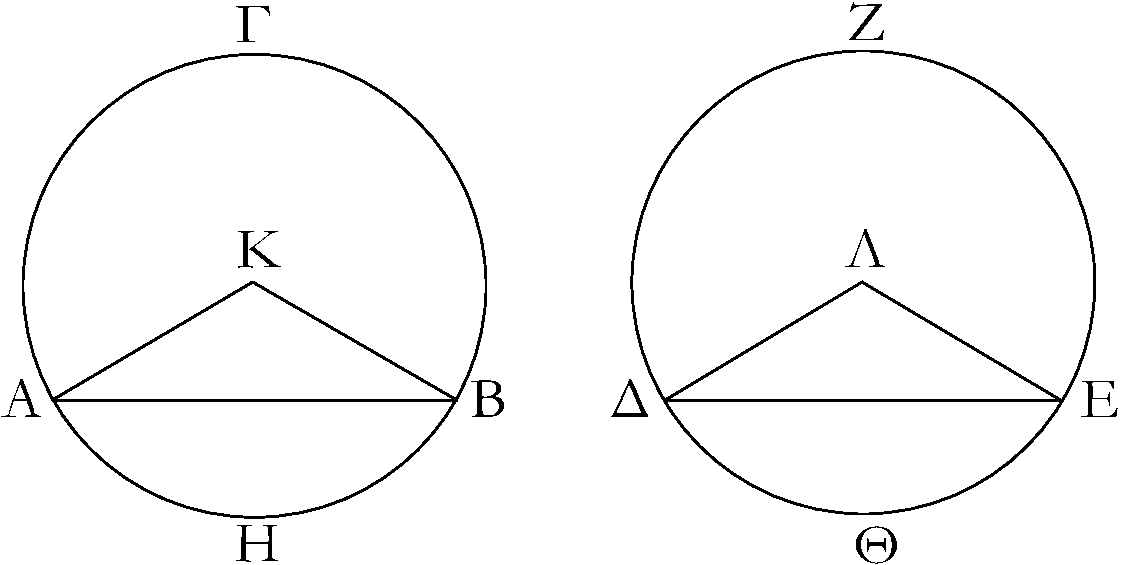
\includegraphics{Book03/fig28g.eps}}

\gr{Εἰλήφθω γὰρ τὰ κέντρα τῶν κύκλων τὰ Κ, Λ, καὶ ἐπεζεύθθωσαν αἱ
ΑΚ, ΚΒ, ΔΛ, ΛΕ.}

\gr{Καὶ ἐπεὶ >ίσοι κύκλοι εἰσίν, >ίσαι εἰσὶ καὶ αἱ ἐκ τῶν κέντρων;
δύο δὴ αἱ ΑΚ, ΚΒ δυσὶ ταῖξ ΔΛ, ΛΕ
>ίσαι εἰσίν; καὶ βάσιξ ἡ ΑΒ βάσει τῆ| ΔΕ >ίση; γωνία >άρα ἡ ὑπὸ
ΑΚΒ γωνίᾳ τῆ| ὑπὸ ΔΛΕ >ίση ἐστίν. αἱ δὲ >ίσαι γωνίαι ἐπὶ
>ίσων περιφερειῶν βεβήκασιν, <όταν πρὸξ τοῖξ κέντροιξ >ῶσιν; >ίση
>άρα ἡ ΑΗΒ περιφέρεια τῆ| ΔJΕ. ἐστὶ δὲ καὶ <όλοξ ὁ ΑΒΓ
κύκλοξ <όλῳ τῶ| ΔΕΖ κύκλῳ >ίσοξ; καὶ λοιπὴ >άρα ἡ ΑΓΒ 
περιφέρεια λοιπῆ| τῆ| ΔΖΕ περιφερείᾳ >ίση ἐστίν.}

\gr{Ἐν >άρα τοῖξ >ίσοιξ κύκλοιξ αἱ >ίσαι εὐθεῖαι >ίσαξ περιφερείαξ ἀφαιροῦσι
τὴν μὲν μείζονα τῆ| μείζονι τὴν δὲ ἐλάττονα τῆ| ἐλάττονι; <όπερ
>έδει δεῖχαι.}}

\ParallelRText{
\begin{center}
{\large Proposition 28}
\end{center}

 In equal circles, equal straight-lines cut off equal circumferences, 
the greater (circumference being equal) to the greater, and the lesser to the lesser.

Let $ABC$ and $DEF$ be equal circles, and let $AB$ and $DE$ be equal straight-lines
in these circles, cutting off the greater circumferences $ACB$ and $DFE$, 
and the lesser (circumferences) $AGB$ and $DHE$ (respectively). I say that
the greater circumference $ACB$ is equal to the greater circumference $DFE$,
and the lesser circumference $AGB$ to (the lesser) $DHE$.

\epsfysize=1.6in
\centerline{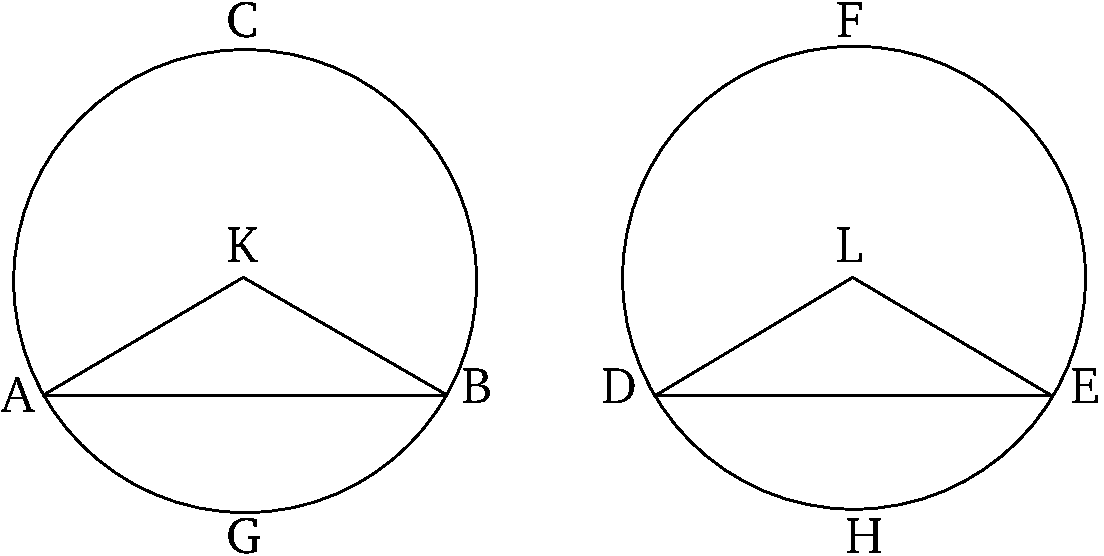
\includegraphics{Book03/fig28e.eps}}

For let the centers of the circles, $K$ and $L$, be found [Prop.~3.1],
and let $AK$, $KB$, $DL$, and $LE$ be joined.

And since ($ABC$ and $DEF$) are equal circles, their radii are also equal [Def.~3.1]. So the two
(straight-lines) $AK$, $KB$ are equal to the two (straight-lines) $DL$, $LE$ (respectively).
And the base $AB$ (is) equal to the base $DE$. Thus, angle $AKB$ is equal
to angle $DLE$ [Prop.~1.8]. And equal angles stand upon equal circumferences,
when they are at the centers [Prop.~3.26]. Thus, circumference $AGB$
(is) equal to $DHE$. And the whole circle $ABC$ is also equal to the whole
circle $DEF$. Thus, the remaining circumference $ACB$
is also equal to the remaining circumference $DFE$.

Thus, in equal circles, equal straight-lines cut off equal circumferences, 
the greater (circumference being equal) to the greater, and the lesser to the lesser. (Which is) the very thing it was required to show.}
\end{Parallel}

%%%%%%
% Prop 3.29
%%%%%%
\pdfbookmark[1]{Proposition 3.29}{pdf3.29}
\begin{Parallel}{}{} 
\ParallelLText{
\begin{center}
{\large \ggn{29}.}
\end{center}\vspace*{-7pt}

\gr{Ἐν τοῖξ >ίσοιξ κύκλοιξ τὰξ >ίσαξ περιφερείαξ >ίσαι εὐθεῖαι ὑποτείνουσιν.}

\gr{>'Εστωσαν >ίσοι κύκλοι οἱ ΑΒΓ, ΔΕΖ, καὶ ἐν α\kern -.7pt  ὐτοῖξ >ίσαι περιφέρειαι
ἀπειλήφθωσαν αἱ ΒΗΓ, ΕJΖ, καὶ ἐπεζεύθθωσαν αἱ ΒΓ, ΕΖ εὐθεῖαι;
λέγω, <ότι >ίση ἐστὶν ἡ ΒΓ τῆ| ΕΖ.}

\gr{Εἰλήφθω γὰρ τὰ κέντρα τῶν κύκλων, καὶ >έστω τὰ Κ, Λ, καὶ ἐπεζεύθθωσαν αἱ ΒΚ, ΚΓ, ΕΛ, ΛΖ.}

\gr{Καὶ ἐπεὶ >ίση ἐστὶν ἡ ΒΗΓ περιφέρεια τῆ| ΕJΖ περιφερείᾳ, >ίση
ἐστὶ καὶ γωνία ἡ ὑπὸ ΒΚΓ τῆ| ὑπὸ ΕΛΖ. καὶ ἐπεὶ >ίσοι
εἰσὶν οἱ ΑΒΓ, ΔΕΖ κύκλοι, >ίσαι εἰσὶ καὶ αἱ ἐκ τῶν κέντρων;
δύο δὴ αἱ ΒΚ, ΚΓ δυσὶ ταῖξ ΕΛ, ΛΖ >ίσαι εἰσίν; καὶ γωνίαξ
>ίσαξ περιέθουσιν; βάσιξ >άρα ἡ ΒΓ βάσει τῆ| ΕΖ >ίση ἐστίν;}\\~\\~\\~\\

\epsfysize=1.7in
\centerline{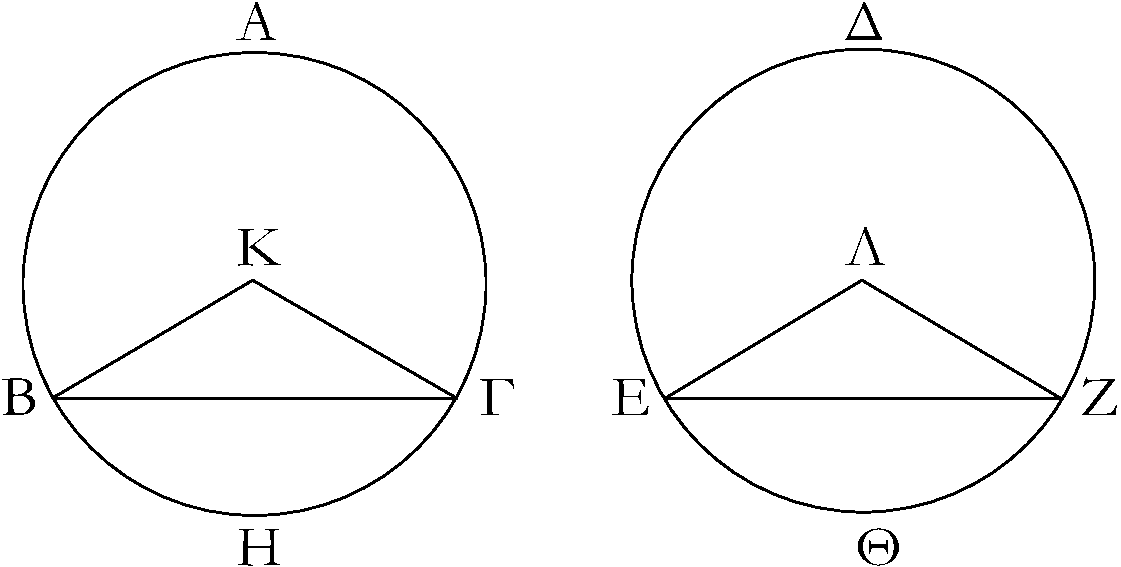
\includegraphics{Book03/fig29g.eps}}

\gr{Ἐν >άρα τοῖξ >ίσοιξ κύκλοιξ τὰξ >ίσαξ περιφερείαξ
>ίσαι εὐθεῖαι ὑποτείνουσιν; <όπερ >έδει δεῖχαι.}}

\ParallelRText{
\begin{center}
{\large Proposition 29}
\end{center}

In equal circles, equal straight-lines subtend equal circumferences.

Let $ABC$ and $DEF$ be equal circles, and within them let the equal circumferences $BGC$ and $EHF$ be cut off. And let the straight-lines $BC$ and $EF$ be joined. I say that $BC$ is equal to $EF$.

For let the centers of the circles be found [Prop.~3.1], and
let them be (at) $K$ and $L$. And let $BK$, $KC$, $EL$, and $LF$ be joined.

And since the circumference $BGC$ is equal to the circumference $EHF$,
the angle $BKC$ is also equal to (angle) $ELF$ [Prop.~3.27]. And since the circles
$ABC$ and $DEF$ are equal, their radii are also equal [Def.~3.1]. 
So the two (straight-lines) $BK$, $KC$ are equal to the two (straight-lines)
$EL$, $LF$ (respectively). And they contain equal angles. Thus, the
base $BC$ is equal to the base $EF$ [Prop.~1.4].

\epsfysize=1.7in
\centerline{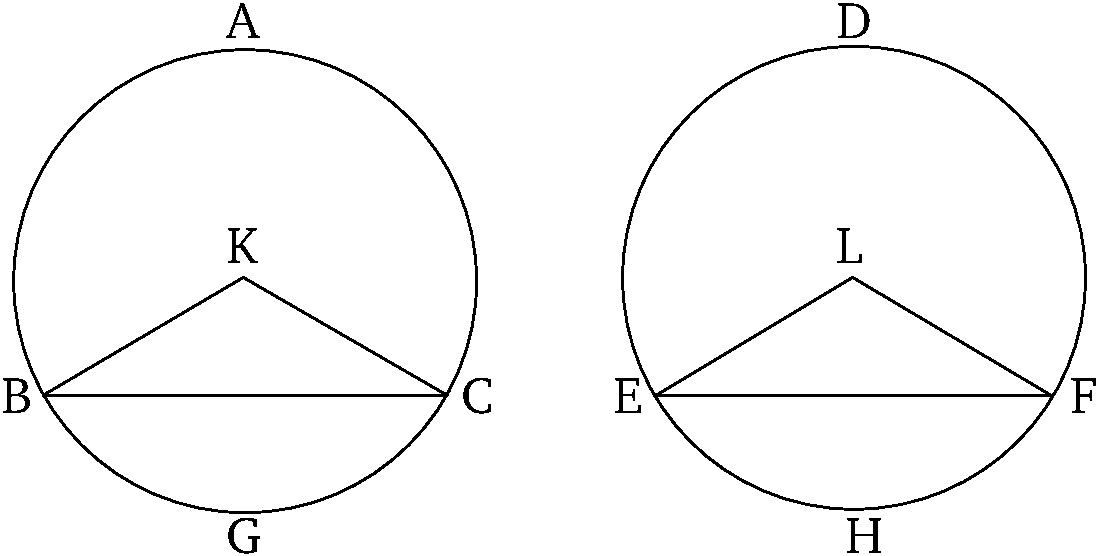
\includegraphics{Book03/fig29e.eps}}

Thus,  in equal circles, equal straight-lines subtend equal circumferences.
(Which is) the very thing it was required to show.}
\end{Parallel}

%%%%%%
% Prop 3.30
%%%%%%
\pdfbookmark[1]{Proposition 3.30}{pdf3.30}
\begin{Parallel}{}{} 
\ParallelLText{
\begin{center}
{\large \ggn{30}.}
\end{center}\vspace*{-7pt}

\gr{Τὴν δοθεῖσαν περιφέρειαν δίθα τεμεῖν.}

\gr{>'Εστω ἡ δοθεῖσα περιφέρεια ἡ ΑΔΒ; δεῖ δὴ τὴν ΑΔΒ περιφέρειαν
δίθα τεμεῖν.}

\gr{Ἐπεζεύθθω ἡ ΑΒ, καὶ τετμ\kern -.7pt  ήσθω δίθα κατὰ τὸ Γ, καὶ ἀπὸ τοῦ
Γ σημείου τῆ| ΑΒ εὐθείᾳ πρὸξ ὀρθὰξ >ήθθω ἡ ΓΔ, καὶ ἐπεζεύθθωσαν αἱ ΑΔ, ΔΒ.}

\epsfysize=1.3in
\centerline{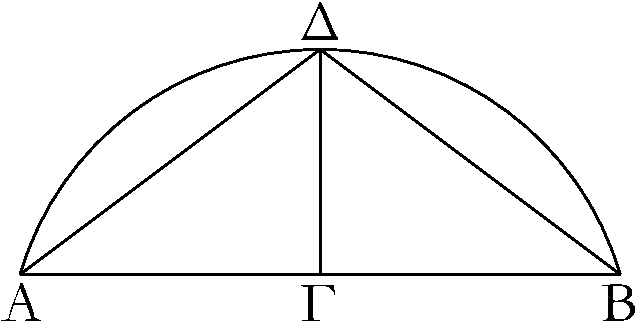
\includegraphics{Book03/fig30g.eps}}

\gr{Καὶ ἐπεὶ >ίση ἐστὶν ἡ ΑΓ τῆ| ΓΒ, κοινὴ δὲ ἡ ΓΔ, δύο δὴ
αἱ ΑΓ, ΓΔ δυσὶ ταῖξ ΒΓ, ΓΔ >ίσαι εἰσίν; καὶ γωνία ἡ ὑπὸ
ΑΓΔ γωνίᾳ τῆ| ὑπὸ ΒΓΔ >ίση; ὀρθὴ γὰρ ἑκατέρα; βάσιξ
>άρα ἡ ΑΔ βάσει τῆ| ΔΒ >ίση ἐστίν. αἱ δὲ >ίσαι εὐθεῖαι >ίσαξ περιφερείαξ ἀφαιροῦσι τὴν μὲν μείζονα τῆ| μείζονι τὴν δὲ
ἐλάττονα τῆ| ἐλάττονι; κάι ἐστιν ἑκατέρα τῶν ΑΔ, ΔΒ περιφερειῶν
ἐλάττων ἡμικυκλίου; >ίση >άρα ἡ ΑΔ περιφέρεια τῆ| ΔΒ περιφερείᾳ.}

\gr{Ἡ >άρα δοθεῖσα περιφέρεια δίθα τέτμ\kern -.7pt  ηται κατὰ τὸ Δ σημεῖον; <όπερ
>έδει ποιῆσαι.}}

\ParallelRText{
\begin{center}
{\large Proposition 30}
\end{center}

To cut a given circumference in half.

Let $ADB$ be the given circumference. So it is required to cut circumference
$ADB$ in half.

Let $AB$ be joined, and let it be cut in half at (point) $C$ [Prop.~1.10]. And let $CD$ be drawn from point $C$, at right-angles
to $AB$ [Prop.~1.11]. And let $AD$, and $DB$ be joined.

\epsfysize=1.3in
\centerline{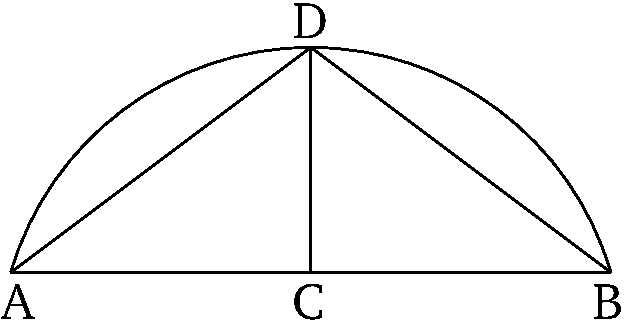
\includegraphics{Book03/fig30e.eps}}

And since $AC$ is equal to $CB$, and $CD$ (is) common, the two
(straight-lines) $AC$, $CD$ are equal to the two (straight-lines) $BC$, $CD$ (respectively).
And angle $ACD$ (is) equal to angle $BCD$. For (they are) each right-angles.
Thus, the base $AD$ is equal to the base $DB$ [Prop.~1.4]. And equal
straight-lines cut off equal circumferences, the greater (circumference being
equal) to the greater, and the lesser to the lesser [Prop.~1.28].
And the circumferences $AD$ and $DB$ are each less than a semi-circle.
Thus, circumference $AD$ (is) equal to circumference $DB$.

Thus, the given circumference has been cut in half at point $D$. (Which is)
the very thing it was required to do. }
\end{Parallel}

%%%%%%
% Prop 3.31
%%%%%%
\pdfbookmark[1]{Proposition 3.31}{pdf3.31}
\begin{Parallel}{}{} 
\ParallelLText{
\begin{center}
{\large \ggn{31}.}
\end{center}\vspace*{-7pt}

\gr{Ἐν κύκλῳ ἡ μὲν ἐν τῶ| ἡμικυκλίῳ γωνία ὀρθή ἐστιν, ἡ δὲ
ἐν τῶ| μείζονι τμ\kern -.7pt  ήματι ἐλάττων ὀρθῆξ, ἡ δὲ ἐν τῶ| ἐλάττονι
τμ\kern -.7pt  ήματι μείζων ὀρθῆξ; καὶ >έπι ἡ μὲν τοῦ μείζονοξ τμ\kern -.5pt  ήματοξ γωνία μείζων ἐστὶν ὀρθῆξ, ἡ δὲ τοῦ ἐλάττονοξ τμ\kern -.3pt  ήματοξ γωνία
ἐλάττων ὀρθῆξ.}\\

\epsfysize=2.2in
\centerline{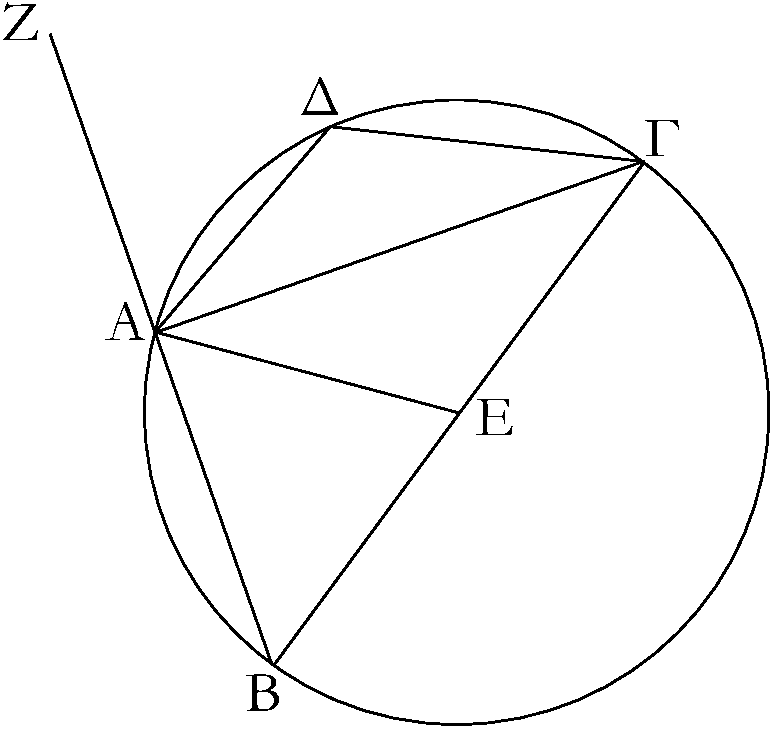
\includegraphics{Book03/fig31g.eps}}

\gr{>'Εστω κύκλοξ ὁ ΑΒΓΔ, διάμετροξ δὲ α\kern -.7pt  ὐτοῦ >έστω ἡ ΒΓ,
κέντρον δὲ τὸ Ε, καὶ ἐπεζεύθθωσαν αἱ ΒΑ, ΑΓ, ΑΔ, ΔΓ; λέγω,
<ότι ἡ μὲν ἐν τῶ| ΒΑΓ ἡμικυκλίῳ γωνία ἡ ὑπὸ ΒΑΓ ὀρθή
ἐστιν, ἡ δὲ ἐν τῶ| ΑΒΓ μείζονι τοῦ ἡμικυκλίου τμ\kern -.7pt  ήματι
γωνία ἡ ὑπὸ ΑΒΓ ἐλάττων ἐστὶν ὀρθῆξ, ἡ δὲ ἐν τῶ| ΑΔΓ
ἐλάττονι τοῦ ἡμικυκλίου τμ\kern -.5pt  ήματι γωνία ἡ ὑπὸ ΑΔΓ μείζων
ἐστὶν ὀρθῆξ.}

\gr{Ἐπεζεύθθω ἡ ΑΕ, καὶ διήθθω ἡ ΒΑ ἐπὶ τὸ Ζ.}

\gr{Καὶ ἐπεὶ >ίση ἐστὶν ἡ ΒΕ τῆ| ΕΑ, >ίση ἐστὶ καὶ γωνία ἡ ὑπὸ
ΑΒΕ τῆ| ὑπὸ ΒΑΕ. πάλιν, ἐπεὶ >ίση ἐστὶν ἡ ΓΕ τῆ| ΕΑ, >ίση
ἐστὶ καὶ ἡ ὑπὸ ΑΓΕ τῆ| ὑπὸ ΓΑΕ; <όλη >άρα ἡ ὑπὸ ΒΑΓ
δυσὶ ταῖξ ὑπὸ ΑΒΓ, ΑΓΒ >ίση ἐστίν. ἐστὶ δὲ καὶ ἡ ὑπὸ 
ΖΑΓ ἐκτὸξ τοῦ ΑΒΓ τριγώνου δυσὶ ταῖξ ὑπὸ ΑΒΓ, ΑΓΒ γωνίαιξ
>ίση; >ίση >άρα καὶ ἡ ὑπὸ ΒΑΓ γωνία τῆ| ὑπὸ ΖΑΓ;
ὀρθὴ >άρα ἑκατέρα; ἡ >άρα ἐν τῶ| ΒΑΓ ἡμικυκλίῳ 
γωνία ἡ ὑπὸ ΒΑΓ ὀρθή ἐστιν.}

\gr{Καὶ ἐπεὶ τοῦ ΑΒΓ τρίγωνου δύο γωνίαι αἱ ὑπὸ ΑΒΓ, ΒΑΓ δύο
ὀρθῶν ἐλάττονέξ εἰσιν, ὀρθὴ δὲ ἡ ὑπὸ ΒΑΓ, ἐλάττων >άρα
ὀρθῆξ ἐστιν ἡ ὑπὸ ΑΒΓ γωνία; καί ἐστιν ἐν τῶ| ΑΒΓ μείζονι
τοῦ ἡμικυκλίου τμ\kern -.7pt  ήματι.}

\gr{Καὶ ἐπεὶ ἐν κύκλῳ τετράπλευρόν ἐστι τὸ ΑΒΓΔ, τῶν δὲ ἐν τοῖξ
κύκλοιξ τετραπλεύρων αἱ ἀπεναντίον γωνίαι δυσὶν ὀρθαῖξ >ίσαι
εἰσίν [αἱ >άρα ὑπὸ ΑΒΓ, ΑΔΓ γωνίαι δυσὶν ὀρθαῖξ >ίσαξ
εἰσίν], καί ἐστιν ἡ ὑπὸ ΑΒΓ ἐλάττων ὀρθῆξ; λοιπὴ >άρα ἡ ὑπὸ
ΑΔΓ γωνία μείζων ὀρθῆξ ἐστιν; καί ἐστιν ἐν τῶ| ΑΔΓ
ἐλάττονι τοῦ ἡμικυκλίου τμ\kern -.7pt  ήματι.}

\gr{Λέγω, <ότι καὶ ἡ μὲν τοῦ μείζονοξ τμ\kern -.7pt  ήματοξ γωνία ἡ περιεθομένη
ὑπό [τε] τῆξ ΑΒΓ περιφερείαξ καὶ τῆξ ΑΓ εὐθείαξ μείζων ἐστὶν
ὀρθῆξ, ἡ δὲ τοῦ ἐλάττονοξ τμ\kern -.7pt  ήματοξ γωνία ἡ περιεθομένη
ὑπό [τε] τῆξ ΑΔ[Γ] περιφερείαξ καὶ τῆξ ΑΓ εὐθείαξ ἐλάττων ἐστὶν
ὀρθῆξ. καί ἐστιν α\kern -.5pt  ὐτόθεν φανερόν. ἐπεὶ γὰρ ἡ ὑπὸ τῶν ΒΑ,
ΑΓ εὐθειῶν ὀρθή ἐστιν, ἡ >άρα ὑπὸ τῆξ ΑΒΓ περιφερείαξ καὶ τῆξ
ΑΓ εὐθείαξ περιεθομένη μείζων ἐστὶν ὀρθῆξ. πάλιν, ἐπεὶ
ἡ ὑπὸ τῶν ΑΓ, ΑΖ εὐθειῶν ὀρθή ἐστιν, ἡ >άρα ὑπὸ
τῆξ ΓΑ εὐθείαξ καὶ τῆξ ΑΔ[Γ] περιφερείαξ περιεθομένη ἐλάττων
ἐστὶν ὀρθῆξ.}

\gr{Ἐν κύκλῳ >άρα ἡ μὲν ἐν τῶ| ἡμικυκλίῳ γωνία ὀρθή ἐστιν, ἡ δὲ
ἐν τῶ| μείζονι τμ\kern -.7pt  ήματι ἐλάττων ὀρθῆξ, ἡ δὲ ἐν τῶ| ἐλάττονι
[τμ\kern -.7pt  ήματι] μείζων ὀρθῆξ; καὶ >έπι ἡ μὲν τοῦ μείζονοξ τμ\kern -.5pt  ήματοξ [γωνία] μείζων [ἐστὶν] ὀρθῆξ, ἡ δὲ τοῦ ἐλάττονοξ τμ\kern -.3pt  ήματοξ [γωνία] ἐλάττων ὀρθῆξ; <όπερ >έδει δεῖχαι.}}

\ParallelRText{
\begin{center}
{\large Proposition 31}
\end{center}

In a circle, the angle in a semi-circle is a right-angle, and that in a
greater segment (is) less than a right-angle, and that in a
lesser segment (is) greater than a right-angle. And, further, the angle of
a segment greater (than a semi-circle) is greater than a right-angle, and
the angle of a segment less (than a semi-circle) is less than a right-angle.

\epsfysize=2.2in
\centerline{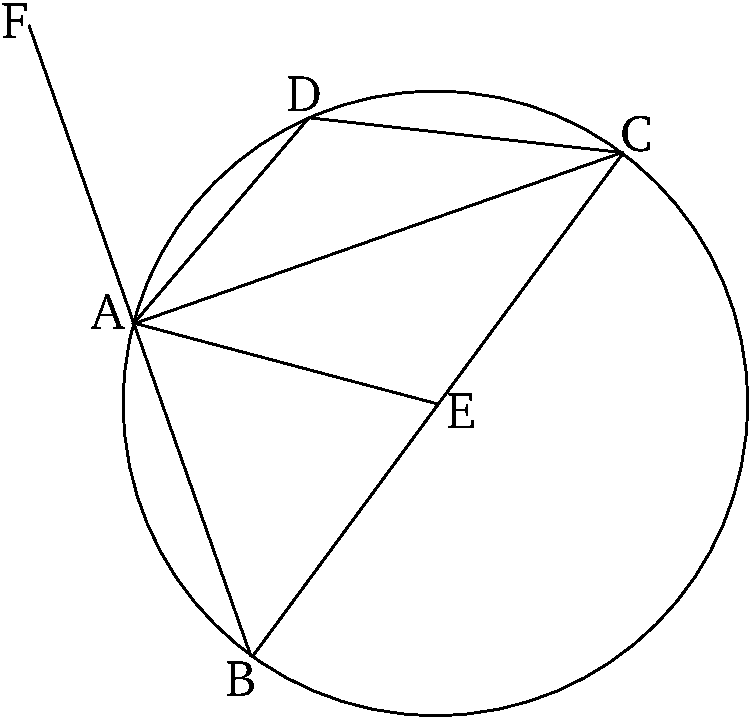
\includegraphics{Book03/fig31e.eps}}

Let $ABCD$  be a circle, and let $BC$ be its diameter, and $E$ its center. And let $BA$, $AC$, $AD$, and $DC$ be joined. I say that the angle $BAC$ in the semi-circle $BAC$ is a right-angle, and the angle $ABC$ in the segment $ABC$, (which is) greater than a semi-circle, is less
than a right-angle, and the angle $ADC$ in the segment $ADC$, (which is) less than a semi-circle,
is greater than a right-angle.

Let $AE$ be joined, and let $BA$ be drawn through to $F$.

And since $BE$ is equal to $EA$, angle $ABE$ is also equal to $BAE$ [Prop.~1.5]. Again, since $CE$ is equal to $EA$, $ACE$ is also equal to  $CAE$ [Prop.~1.5].
Thus, the whole (angle) $BAC$ is equal to the two (angles) $ABC$ and $ACB$.
And $FAC$, (which is) external to triangle $ABC$, is also equal to the two angles
$ABC$ and $ACB$ [Prop.~1.32]. Thus, angle $BAC$ (is) also equal to
$FAC$. Thus, (they are) each right-angles. [Def.~1.10]. Thus, the angle
$BAC$ in the semi-circle $BAC$ is a right-angle.

And since the two angles $ABC$ and $BAC$ of triangle $ABC$ are less than 
two right-angles [Prop.~1.17], and $BAC$ is a right-angle, angle $ABC$ is
thus less than a right-angle. And it is in segment $ABC$, (which is) greater 
than
a semi-circle.

And since $ABCD$ is a quadrilateral within a circle, and for quadrilaterals within circles
the (sum of the) opposite angles is equal to two right-angles 
[Prop.~3.22] [angles $ABC$ and $ADC$ are thus equal to two right-angles],
and (angle) $ABC$ is  less than a right-angle. The remaining angle $ADC$
is thus greater than a right-angle. And it is in segment $ADC$, (which is)
less than a semi-circle.

I also say that the angle of the greater segment, (namely) that contained by
the circumference $ABC$ and the straight-line $AC$, is greater than a right-angle.
And the angle of the lesser segment, (namely) that contained by the circumference
$AD[C]$ and the straight-line $AC$, is less than a right-angle. And
this is immediately apparent. For since the (angle contained by) the
two straight-lines $BA$ and $AC$ is a right-angle, the (angle) contained
by the circumference $ABC$ and the straight-line $AC$ is thus greater than a right-angle. Again, since the (angle contained by) the straight-lines
$AC$ and $AF$ is a right-angle, the (angle) contained by the circumference
$AD[C]$ and the straight-line $CA$ is thus less than a right-angle.

Thus, in a circle, the angle in a semi-circle is a right-angle, and that in a
greater segment (is) less than a right-angle, and that in a
lesser [segment] (is) greater than a right-angle. And, further, the [angle] of
a segment greater (than a semi-circle) [is] greater than a right-angle, and
the [angle] of a segment less (than a semi-circle) is  less than a right-angle.
(Which is) the very thing it was required to show.}
\end{Parallel}

%%%%%%
% Prop 3.32
%%%%%%
\pdfbookmark[1]{Proposition 3.32}{pdf3.32}
\begin{Parallel}{}{} 
\ParallelLText{
\begin{center}
{\large \ggn{32}.}
\end{center}\vspace*{-7pt}

\gr{Ἐὰν κύκλου ἐφάπτηταί τιξ εὐθεῖα, ἀπὸ δὲ τῆξ ἁφῆξ εἰξ τὸν κύκλον διαθθῆ| τιξ εὐθεῖα τέμνουσα τὸν κύκλον, <ὰξ ποιεῖ γωνίαξ
πρὸξ τῆ| ἐφαπτομένῃ, >ίσαι >έσονται ταῖξ ἐν τοῖξ ἐναλλὰχ
τοῦ κύκλου τμ\kern -.7pt  ήμασι γωνίαιξ.}\\

\epsfysize=2.1in
\centerline{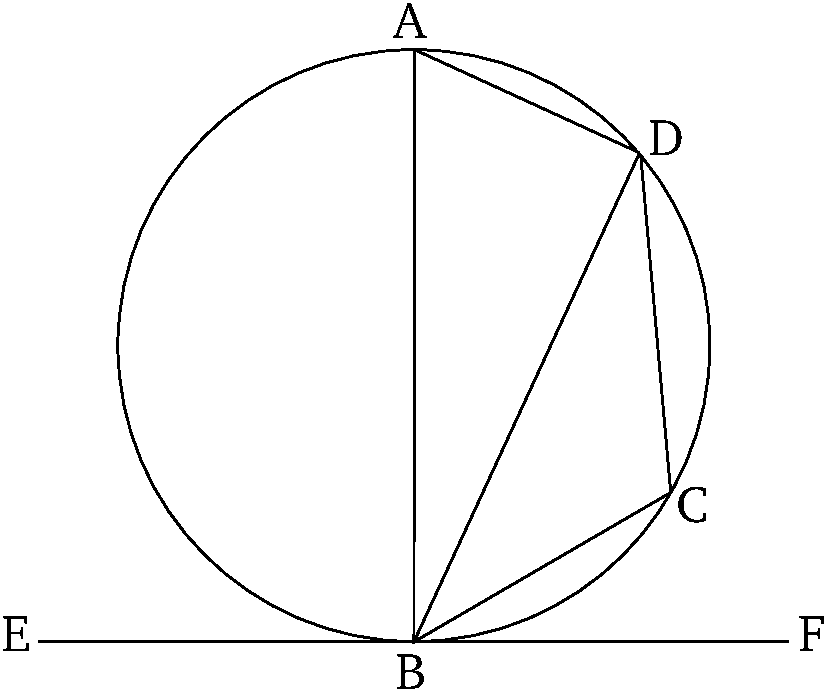
\includegraphics{Book03/fig32e.eps}}

\gr{Κύκλου γὰρ τοῦ ΑΒΓΔ ἐφαπτέσθω τιξ εὐθεῖα ἡ ΕΖ κατὰ τὸ Β σημεῖον, καὶ ἀπὸ τοῦ Β σημείου διήθθω τιξ εὐθεῖα εἰξ τὸν
ΑΒΓΔ κύκλον τέμνουσα α\kern -.7pt  ὐτὸν ἡ ΒΔ. λέγω, <ότι <ὰξ ποιεῖ γωνίαξ
ἡ ΒΔ μετὰ τῆξ ΕΖ  ἐφαπτομένηξ, >ίσαξ >έσονται ταῖξ ἐν τοῖξ
ἐναλλὰχ τμ\kern -.7pt  ήμασι τοῦ κύκλου γωνίαιξ, τουτέστιν, <ότι ἡ μὲν
ὑπὸ ΖΒΔ γωνία >ίση ἐστὶ τῆ| ἐν τῶ| ΒΑΔ τμ\kern -.5pt  ήματι συνισταμένῃ γωνίᾳ, ἡ δὲ ὑπὸ ΕΒΔ γωνία >ίση ἐστὶ τῆ| ἐν τῶ| ΔΓΒ τμ\kern -.3pt  ήματι συνισταμένῃ γωνίᾳ.}

\gr{>'Ηθθω γὰρ ἀπὸ τοῦ Β τῆ| ΕΖ πρὸξ ὀρθὰξ ἡ ΒΑ, καὶ εἰλήφθω ἐπὶ
τῆξ ΒΔ περιφερείαξ τυθὸν σημεῖον τὸ Γ, καὶ ἐπεζεύθθωσαν αἱ ΑΔ, ΔΓ, ΓΒ.}

\gr{Καὶ ἐπεὶ κύκλου τοῦ ΑΒΓΔ ἐφάπτεταί τιξ εὐθεῖα ἡ ΕΖ κατὰ
τὸ Β, καὶ ἀπὸ τῆξ ἁφῆξ >ῆκται τῆ| ἐφαπτομένῃ πρὸξ ὀρθὰξ ἡ ΒΑ, ἐπὶ τῆξ ΒΑ >άρα τὸ κέντρον ἐστὶ τοῦ ΑΒΓΔ κύκλου. ἡ ΒΑ
>άρα διάμετόξ ἐστι τοῦ ΑΒΓΔ κύκλου; ἡ >άρα ὑπὸ ΑΔΒ γωνία
ἐν ἡμικυκλίῳ ο>ῦσα ὀρθή ἐστιν. λοιπαὶ >άρα αἱ ὑπὸ ΒΑΔ, ΑΒΔ
μιᾶ| ὀρθῆ| >ίσαι εἰσίν. ἐστὶ δὲ καὶ ἡ ὑπὸ ΑΒΖ ὀρθή; ἡ >άρα ὑπὸ ΑΒΖ >ίση ἐστὶ ταῖξ ὑπὸ ΒΑΔ, ΑΒΔ. κοινὴ ἀφῃρήσθω ἡ ὑπὸ
ΑΒΔ; λοιπὴ >άρα ἡ ὑπὸ ΔΒΖ γωνία >ίση ἐστὶ τῆ| ἐν τῶ| ἐναλλὰχ τμ\kern -.7pt  ήματι τοῦ κύκλου γωνίᾳ τῆ| ὑπὸ ΒΑΔ. καὶ ἐπεὶ ἐν κύκλῳ
τετράπλευρόν ἐστι τὸ ΑΒΓΔ, αἱ ἀπεναντίον α\kern -.7pt  ὐτοῦ γωνίαι δυσὶν
ὀρθαῖξ >ίσαι  εἰσίν. εἰσὶ δὲ καὶ αἱ ὑπὸ ΔΒΖ, ΔΒΕ δυσὶν ὀρθαῖξ
>ίσαι;
 αἱ >άρα ὑπὸ ΔΒΖ, ΔΒΕ ταῖξ ὑπὸ ΒΑΔ, ΒΓΔ >ίσαι
εἰσίν, ~ὡν ἡ ὑπὸ ΒΑΔ τῆ| ὑπὸ ΔΒΖ ἐδείθθη >ίση;
λοιπὴ >άρα ἡ ὑπὸ ΔΒΕ τῆ| ἐν τῶ| ἐναλλὰχ τοῦ κύκλου τμ\kern -.5pt  ήματι
τῶ| ΔΓΒ τῆ| ὑπὸ ΔΓΒ γωνίᾳ ἐστὶν >ίση.}

\gr{Ἐὰν >άρα κύκλου ἐφάπτηταί τιξ εὐθεῖα, ἀπὸ δὲ τῆξ ἁφῆξ εἰξ τὸν κύκλον διαθθῆ| τιξ εὐθεῖα τέμνουσα τὸν κύκλον, <ὰξ ποιεῖ γωνίαξ
πρὸξ τῆ| ἐφαπτομένῃ, >ίσαι >έσονται ταῖξ ἐν τοῖξ ἐναλλὰχ
τοῦ κύκλου τμ\kern -.7pt  ήμασι γωνίαιξ; <όπερ >έδει δεῖχαι.}}

\ParallelRText{
\begin{center}
{\large Proposition 32}
\end{center}

If some straight-line touches a circle, and some (other) straight-line is drawn  
across, from the point of contact into the circle,  cutting the circle (in two), (then) those angles  the (straight-line) makes
with the tangent will be equal to the angles in
the alternate segments of the circle.

\epsfysize=2.1in
\centerline{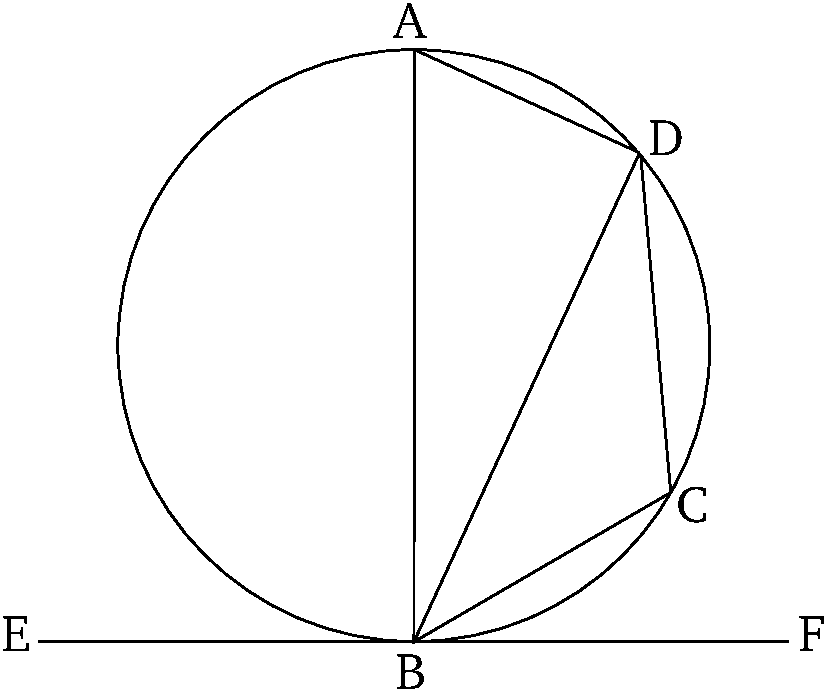
\includegraphics{Book03/fig32e.eps}}

For let some straight-line $EF$ touch the circle $ABCD$ at the point $B$, and let
some (other) straight-line $BD$ be drawn from point $B$ into the
circle $ABCD$, cutting it (in two). I say that the angles $BD$ makes with the tangent 
$EF$  will be equal to the angles in the alternate segments of the circle.
That is to say, that angle $FBD$ is equal to the angle constructed
in segment $BAD$, and angle $EBD$ is equal to the angle constructed in segment $DCB$.

For let $BA$ be drawn from $B$, at right-angles to $EF$ [Prop.~1.11].
And let the point $C$ be taken at random on the circumference $BD$. And
let $AD$, $DC$, and $CB$ be joined.

And since some straight-line $EF$ touches the circle $ABCD$ at point $B$, and
$BA$ has been drawn from the point of contact, at right-angles to the
tangent, the center of circle $ABCD$ is thus on $BA$ [Prop.~3.19].
Thus, $BA$ is a diameter of circle $ABCD$.
Thus, angle $ADB$, being in a semi-circle, is a right-angle [Prop.~3.31].
Thus, the remaining angles (of triangle $ADB$) $BAD$ and $ABD$ are equal to one right-angle [Prop.~1.32]. And $ABF$ is also a right-angle. Thus,
$ABF$ is equal to $BAD$ and $ABD$. Let $ABD$ be subtracted from both.
Thus, the remaining angle $DBF$ is equal to the angle $BAD$ in the alternate
segment of the circle. And since $ABCD$ is a quadrilateral in a circle,
(the sum of) its opposite angles is equal to two right-angles [Prop.~3.22]. And $DBF$ and $DBE$ is also equal to two right-angles [Prop.~1.13]. Thus, $DBF$ and $DBE$ is equal to $BAD$ and $BCD$, of which
$BAD$ was shown (to be) equal to $DBF$. Thus, the remaining (angle) $DBE$ is
equal to the angle $DCB$ in the alternate segment $DCB$ of the circle.

Thus, if some straight-line touches a circle, and some (other) straight-line is drawn  across, from the point of contact into the circle,  cutting the circle (in two), (then) those angles  the (straight-line) makes
with the tangent will be equal to the angles in
the alternate segments of the circle. (Which is) the very thing it was required to
show.}
\end{Parallel}

%%%%%%
% Prop 3.33
%%%%%%
\pdfbookmark[1]{Proposition 3.33}{pdf3.33}
\begin{Parallel}{}{} 
\ParallelLText{
\begin{center}
{\large \ggn{33}.}
\end{center}\vspace*{-7pt}

\gr{Ἐπὶ τῆξ δοθείσηξ εὐθείαξ γράψαι τμ\kern -.7pt  ῆμα κύκλου δεθόμε\-νον γωνίαν >ίσην τῆ| δοθείσῃ γωνίᾳ εὐθυγράμμῳ.}

\epsfysize=1.35in
\centerline{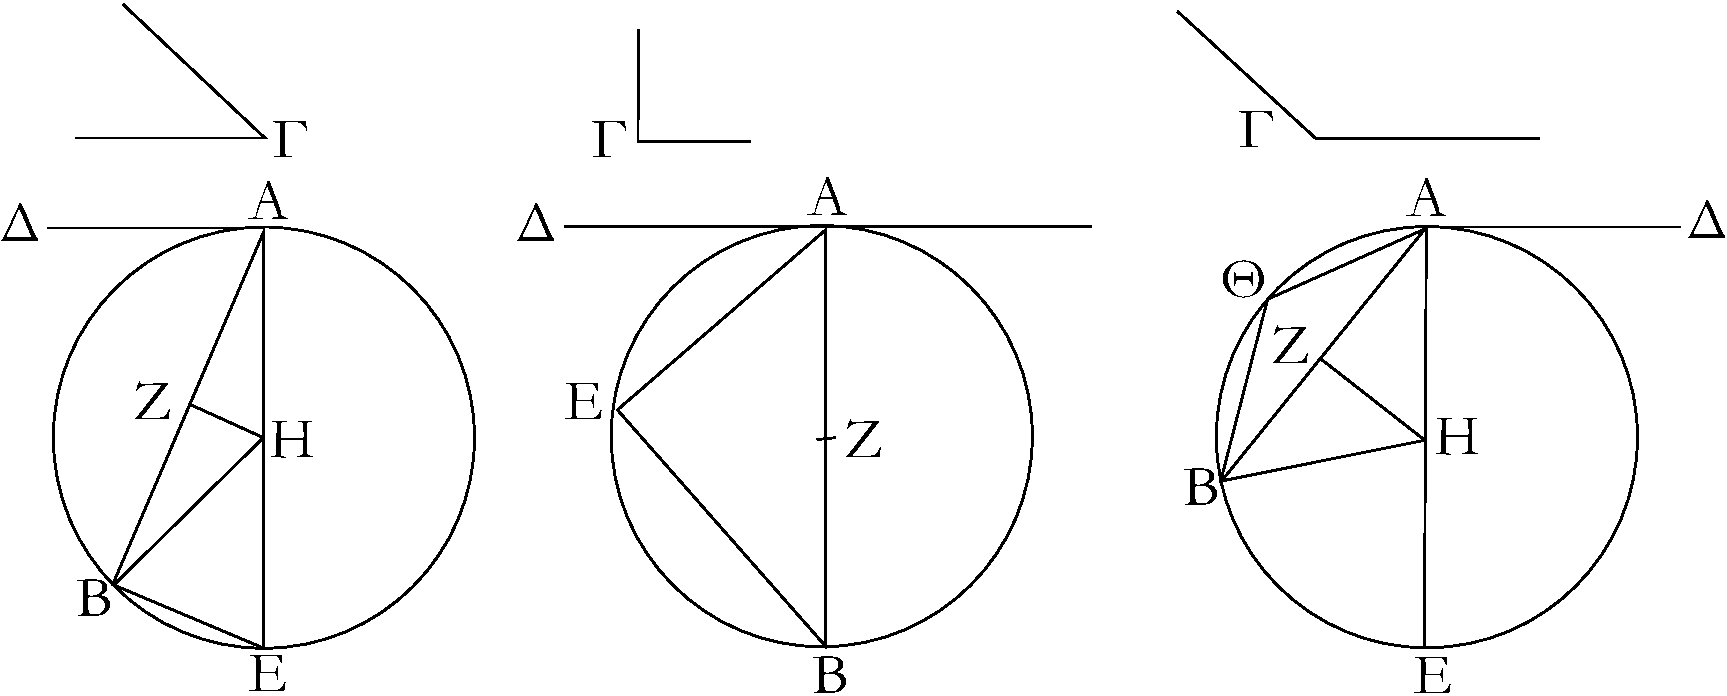
\includegraphics{Book03/fig33g.eps}}

\gr{>'Εστω ἡ δοθεῖσα εὐθεῖα ἡ ΑΒ, ἡ δὲ δοθεῖσα γωνία εὐθύγραμμοξ ἡ
πρὸξ τῶ| Γ; δεῖ δὴ ἐπὶ τῆξ δοθείσηξ εὐθείαξ τῆξ ΑΒ γράψαι τμ\kern -.7pt  ῆμα
κύκλου δεθόμενον γωνίαν >ίσην τῆ| πρὸξ τῶ| Γ.}

\gr{Ἡ δὴ πρὸξ τῶ| Γ [γωνία] >ήτοι ὀχεῖά ἐστιν >ὴ ὀρθὴ >ὴ ἀμβλεῖα;
>έστω πρότερον ὀχεῖα, καὶ ὡξ ἐπὶ τῆξ πρώτηξ καταγραφῆξ συνεστάτω
πρὸξ τῆ| ΑΒ εὐθείᾳ καὶ τῶ| Α σημείῳ τῆ| πρὸξ τῶ| Γ γωνίᾳ
>ίση ἡ ὑπὸ ΒΑΔ; ὀχεῖα >άρα ἐστὶ καὶ ἡ ὑπὸ ΒΑΔ. >ήθθω
τῆ| ΔΑ πρὸξ ὀρθὰξ ἡ ΑΕ, καὶ τετμ\kern -.7pt  ήσθω ἡ ΑΒ δίθα κατὰ τὸ Ζ, καὶ
>ήθθω ἀπὸ τοῦ Ζ σημείου τῆ| ΑΒ πρὸξ ὀρθὰξ ἡ ΖΗ, καὶ
ἐπεζεύθθω ἡ ΗΒ.}

\gr{Καὶ ἐπεὶ >ίση ἐστὶν ἡ ΑΖ τῆ| ΖΒ, κοινὴ δὲ ἡ ΖΗ, δύο δὴ αἱ
ΑΖ, ΖΗ δύο ταῖξ ΒΖ, ΖΗ >ίσαι εἰσίν; καὶ γωνία ἡ ὑπὸ ΑΖΗ [γωνίᾳ]
τῆ| ὑπὸ ΒΖΗ >ίση; βάσιξ >άρα ἡ ΑΗ βάσει τῆ| ΒΗ >ίση ἐστίν. ὁ >άρα κέντρῳ μὲν τῶ| Η διαστήματι δὲ τῶ| ΗΑ κύκλοξ γραφόμενοξ <ήχει καὶ διὰ τοῦ Β. γεγράφθω καὶ >έστω ὁ ΑΒΕ, καὶ ἐπεζεύθθω ἡ ΕΒ.
ἐπεὶ ο>ῦν ἀπ> >άκραξ τῆξ ΑΕ διαμέτρου ἀπὸ τοῦ Α τῆ| ΑΕ πρὸξ ὀρθάξ
ἐστιν ἡ ΑΔ, ἡ ΑΔ >άρα ἐφάπτεται τοῦ ΑΒΕ κύκλου; ἐπεὶ ο>ῦν
κύκλου τοῦ ΑΒΕ ἐφάπτεταί τιξ εὐθεῖα ἡ ΑΔ, καὶ ἀπὸ τῆξ κατὰ
τὸ Α ἁφῆξ  εἰξ τὸν ΑΒΕ κύκλον διῆκταί τιξ εὐθεῖα ἡ ΑΒ, ἡ
>άρα ὑπὸ ΔΑΒ γωνία >ίση ἐστὶ τῆ| ἐν τῶ| ἐναλλὰχ τοῦ 
κύκλου τμ\kern -.7pt  ήματι γωνίᾳ τῆ| ὑπὸ ΑΕΒ. ἀλλ> ἡ ὑπὸ ΔΑΒ τῆ|
πρὸξ τῶ| Γ ἐστιν >ίση; καὶ ἡ πρὸξ τῶ| Γ >άρα γωνία >ίση
ἐστὶ τῆ| ὑπὸ ΑΕΒ.}

\gr{Ἐπὶ τῆξ δοθείσηξ >άρα εὐθείαξ τῆξ ΑΒ τμ\kern -.7pt  ῆμα κύκλου γέγραπται
τὸ ΑΕΒ δεθόμενον γωνίαν τὴν ὑπὸ ΑΕΒ >ίσην τῆ| δοθείσῃ
τῆ| πρὸξ τῶ| Γ.}

\gr{Ἀλλὰ δὴ ὀρθὴ >έστω ἡ πρὸξ τῶ| Γ; καὶ δέον πάλιν >έστω ἐπὶ
τῆξ ΑΒ γράψαι τμ\kern -.7pt  ῆμα κύκλου δεθόμενον γωνίαν >ίσην τῆ| πρὸξ
τῶ| Γ ὀρθῆ| [γωνίᾳ]. συνεστάτω [πάλιν] τῆ| πρὸξ τῶ| Γ ὀρθῆ| γωνίᾳ >ίση ἡ ὑπὸ ΒΑΔ, ὡξ >έθει ἐπὶ τῆξ δευτέραξ καταγραφῆξ, καὶ τετμ\kern -.7pt  ήσθω ἡ ΑΒ δίθα κατὰ τὸ Ζ, καὶ κέντρῳ τῶ| Ζ, διαστήματι δὲ
ὁποτέρῳ τῶν ΖΑ, ΖΒ, κύκλοξ γεγράφθω ὁ ΑΕΒ.}

\gr{Ἐφάπτεται >άρα ἡ ΑΔ εὐθεῖα τοῦ ΑΒΕ κύκλου διὰ τὸ ὀρθὴν ε>ῖναι
τὴν πρὸξ τῶ| Α γωνίαν. καὶ >ίση ἐστὶν ἡ ὑπὸ ΒΑΔ γωνία
τῆ| ἐν τῶ| ΑΕΒ τμ\kern -.7pt  ήματι; ὀρθὴ γὰρ καὶ α\kern -.7pt  ὐτὴ ἐν ἡμικυκλίῳ
ο>ῦσα. ἀλλὰ καὶ ἡ ὑπὸ ΒΑΔ τῆ| πρὸξ τῶ| Γ >ίση ἐστίν. καὶ
ἡ ἐν τῶ| ΑΕΒ >άρα >ίση ἐστὶ  τῆ| πρὸξ τῶ| Γ.}

\gr{Γέγραπται >άρα πάλιν ἐπὶ τῆξ ΑΒ τμ\kern -.7pt  ῆμα κύκλου τὸ ΑΕΒ δεθόμενον
γωνίαν >ίσην τῆ| πρὸξ τῶ| Γ.}

\gr{Ἀλλὰ δὴ ἡ πρὸξ τῶ| Γ ἀμβλεῖα >έστω; καὶ συνεστάτω α\kern -.7pt  ὐτῆ|
>ίση πρὸξ τῆ| ΑΒ εὐθείᾳ καὶ τῶ| Α σημείῳ ἡ ὑπὸ ΒΑΔ, ὡξ
>έθει ἐπὶ τῆξ τρίτηξ καταγραφῆξ, καὶ τῆ| ΑΔ πρὸξ ὀρθὰξ >ήθθω ἡ ΑΕ,
καὶ τετμ\kern -.7pt  ήσθω πάλιν ἡ ΑΒ δίθα κατὰ τὸ Ζ, καὶ τῆ| ΑΒ πρὸξ ὀρθὰξ
>ήθθω ἡ ΖΗ, καὶ ἐπεζεύθθω ἡ ΗΒ.}

\gr{Καὶ ἐπεὶ πάλιν >ίση ἐστὶν ἡ ΑΖ τῆ| ΖΒ, καὶ κοινὴ ἡ ΖΗ, δύο δὴ αἱ
ΑΖ, ΖΗ δύο ταῖξ ΒΖ, ΖΗ >ίσαι εἰσίν; καὶ γωνία ἡ ὑπὸ
ΑΖΗ γωνίᾳ τῆ| ὑπὸ ΒΖΗ >ίση; βάσιξ >άρα ἡ ΑΗ βάσει τῆ| ΒΗ
>ίση ἐστίν; ὁ >άρα κέντρῳ μὲν τῶ| Η διαστήματι δὲ τῶ| ΗΑ κύκλοξ
γραφόμενοξ <ήχει καὶ διὰ τοῦ Β. ἐρθέσθω ὡξ ὁ ΑΕΒ. καὶ ἐπεὶ
τῆ| ΑΕ διαμέτρῳ ἀπ> >άκραξ πρὸξ ὀρθάξ ἐστιν ἡ ΑΔ, ἡ ΑΔ >άρα
ἐφάπτεται τοῦ ΑΕΒ κύκλου. καὶ ἀπὸ τῆξ κατὰ τὸ Α ἐπαφῆξ διῆκται
ἡ ΑΒ; ἡ >άρα ὑπὸ ΒΑΔ γωνία >ίση ἐστὶ τῆ| ἐν τῶ| ἐναλλὰχ τοῦ
κύκλου τμ\kern -.7pt  ήματι  τῶ| ΑJΒ συνισταμένῃ γωνίᾳ. ἀλλ> ἡ ὑπὸ ΒΑΔ γωνία τῆ| πρὸξ τῶ| Γ >ίση ἐστίν. καὶ ἡ ἐν τῶ| ΑJΒ >άρα τμ\kern -.7pt  ήματι
γωνία >ίση  ἐστὶ τῆ| πρὸξ τῶ| Γ.}

\gr{Ἐπὶ τῆξ >άρα δοθείσηξ εὐθείαξ τῆξ ΑΒ γέγραπται τμ\kern -.7pt  ῆμα κύκλου τὸ
ΑJΒ δεθόμενον γωνίαν >ίσην τῆ| πρὸξ τῶ| Γ; <όπερ >έδει ποιῆσαι.}}

\ParallelRText{
\begin{center}
{\large Proposition 33}
\end{center}

To draw a segment of a circle, accepting an angle equal to a given rectilinear angle, on a given straight-line.

\epsfysize=1.53in
\centerline{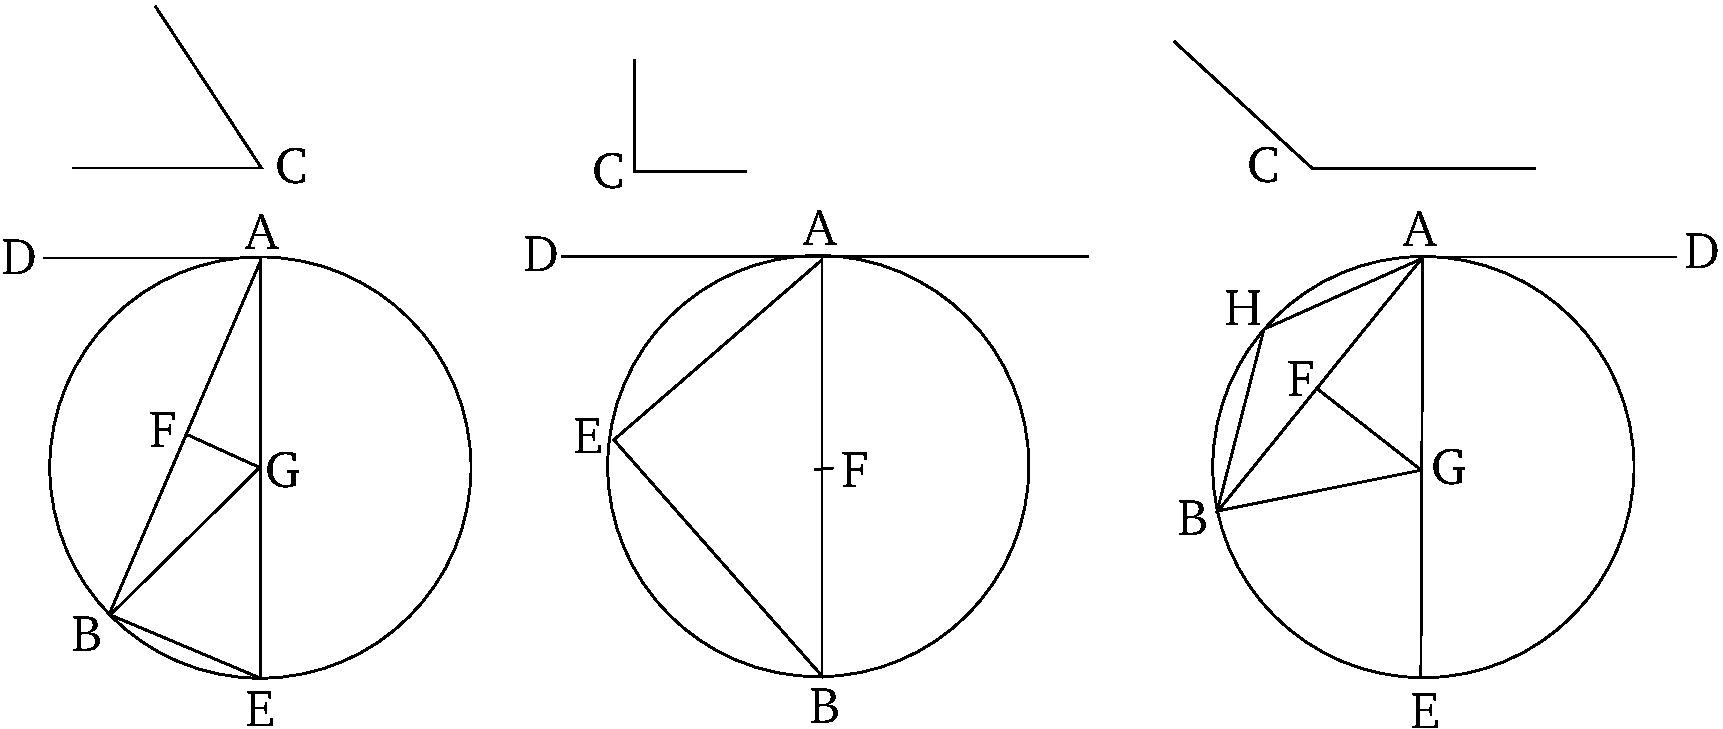
\includegraphics{Book03/fig33e.eps}}

Let $AB$ be the given straight-line, and $C$ the given rectilinear angle. So
it is required to draw a segment of a circle, accepting an angle equal to $C$,
on the given straight-line $AB$.

So the [angle] $C$ is surely either acute, a right-angle, or obtuse. First of all,
let it be acute. And, as in the first diagram (from the left), let (angle) $BAD$,
equal to angle $C$,  be
constructed  on the straight-line $AB$,  at the point A (on it)
[Prop.~1.23]. Thus, $BAD$ is also acute. Let $AE$ be drawn, at
right-angles to $DA$ [Prop.~1.11]. And let $AB$ be cut in half
at $F$ [Prop.~1.10]. And let $FG$ be drawn from point $F$, at right-angles to $AB$
[Prop.~1.11]. And let $GB$ be joined.

And since $AF$ is equal to $FB$, and $FG$ (is) common, the two (straight-lines)
$AF$, $FG$ are equal to the two (straight-lines) $BF$, $FG$ (respectively). And
angle $AFG$ (is) equal to [angle] $BFG$. Thus, the base $AG$ is equal to the
base $BG$ [Prop.~1.4]. Thus, the circle drawn with center $G$, and radius $GA$, will also go through $B$ (as well as $A$). Let it be drawn, and let it be (denoted) $ABE$. And let $EB$ be joined. Therefore, since $AD$ is at the extremity
of diameter $AE$,  (namely, point) $A$,  at right-angles to $AE$, the (straight-line)
$AD$ thus touches the circle $ABE$ [Prop.~3.16~corr.]. Therefore,
since some straight-line $AD$ touches the circle $ABE$, and some (other)
straight-line $AB$ has been drawn across from the point of contact $A$ into circle
$ABE$, angle $DAB$ is thus equal to the angle $AEB$ in the alternate segment of the
circle [Prop.~3.32]. But, $DAB$ is equal to $C$. Thus,
angle $C$ is also equal to $AEB$.

Thus, a segment $AEB$ of a circle, accepting the angle $AEB$ (which is) equal to the
given (angle) $C$, has been drawn on the given straight-line $AB$.

And so let $C$ be a right-angle. And let it again be necessary to draw  a segment
of a circle on $AB$, accepting an angle equal to the right-[angle] $C$. Let the (angle)
$BAD$ [again] be constructed, equal to the right-angle $C$ [Prop.~1.23], as in the second diagram (from the left). And let $AB$ be cut in half at $F$ [Prop.~1.10]. And let the circle $AEB$ be
drawn with center $F$, and radius either  $FA$ or $FB$.

Thus, the straight-line $AD$ touches the circle $ABE$, on account of the angle at $A$ being a right-angle [Prop.~3.16 corr.]. And angle $BAD$ is equal
to the angle in segment $AEB$. For (the latter angle), being in a semi-circle, is also a right-angle [Prop.~3.31]. But,  $BAD$ is also equal to $C$. Thus, the (angle) in (segment) $AEB$ is also equal to $C$.

Thus, a segment $AEB$ of a circle, accepting an angle equal to $C$, has again been
drawn on $AB$.

And so let (angle) $C$ be obtuse. And let (angle) $BAD$, equal
to ($C$), be constructed  on the straight-line $AB$, at the point $A$ 
(on it) [Prop.~1.23], as in the third diagram (from the left). And let $AE$ be
drawn, at right-angles to $AD$ [Prop.~1.11]. And let $AB$ again be 
cut in half at $F$ [Prop.~1.10]. And let $FG$ be drawn,
at right-angles to $AB$ [Prop.~1.10]. And let $GB$ 
be joined.

And again, since $AF$ is equal to $FB$, and $FG$ (is) common, the two (straight-lines) $AF$, $FG$ are equal to the two (straight-lines) $BF$, $FG$ (respectively).
And angle $AFG$ (is) equal to angle $BFG$. Thus, the base $AG$ is equal to
the base $BG$ [Prop.~1.4]. Thus, a circle of center $G$, and radius $GA$,
being drawn, will also go through $B$ (as well as $A$). Let it go like $AEB$ (in the third diagram
from the left). And since $AD$ is at right-angles to the diameter $AE$, at its extremity, $AD$ thus touches circle $AEB$ [Prop.~3.16~corr.]. And $AB$ has been drawn across (the circle) from the point of contact $A$. Thus, angle $BAD$ is equal to the angle constructed in the alternate segment $AHB$ of the circle 
[Prop.~3.32]. But, angle $BAD$ is equal to $C$. Thus, the angle in segment
$AHB$ is also equal to $C$.

Thus, a segment $AHB$ of a circle, accepting an angle equal to $C$, has been
drawn on the given straight-line $AB$. (Which is) the very thing
it was required to do.}
\end{Parallel}

%%%%%%
% Prop 3.34
%%%%%%
\pdfbookmark[1]{Proposition 3.34}{pdf3.34}
\begin{Parallel}{}{} 
\ParallelLText{
\begin{center}
{\large\ggn{34}.}
\end{center}\vspace*{-7pt}

\gr{Ἀπὸ τοῦ δοθέντοξ κύκλου τμ\kern -.7pt  ῆμα ἀφελεῖν δεθόμενον γωνίαν
>ίσην τῆ| δοθείσῃ γωνίᾳ εὐθυγράμμῳ.}

\gr{>'Εστω ὁ δοθεὶξ κύκλοξ ὁ ΑΒΓ, ἡ δὲ δοθεῖσα γωνία εὐθύγραμμοξ
ἡ πρὸξ  τῶ| Δ; δεῖ δὴ ἀπὸ τοῦ ΑΒΓ κύκλου τμ\kern -.7pt  ῆμα ἀφελεῖν
δεθόμενον γωνίαν >ίσην τῆ| δοθείσῃ γωνίᾳ εὐθυγράμμῳ τῆ| πρὸξ
τῶ| Δ.}

\epsfysize=1.8in
\centerline{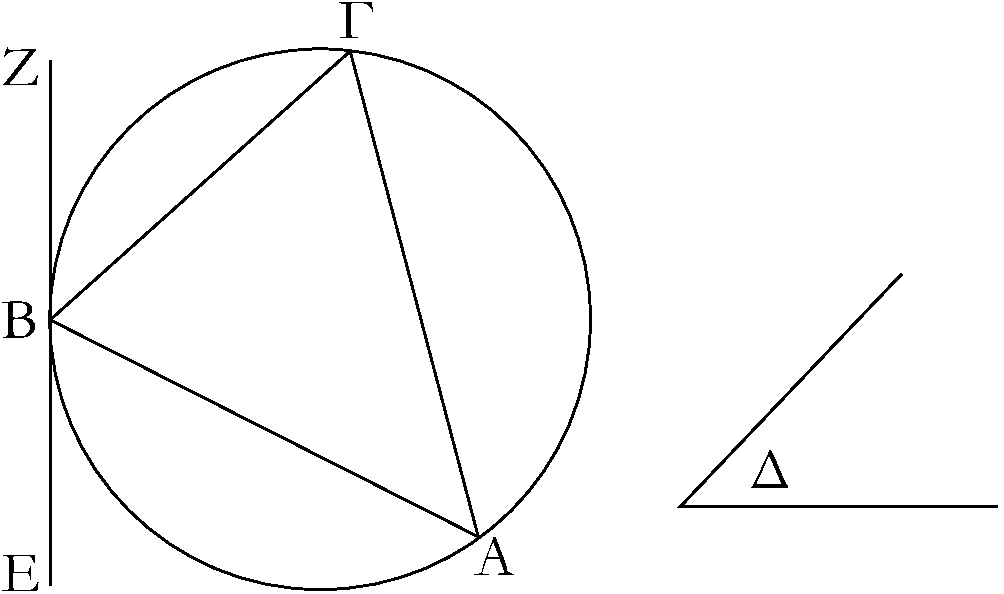
\includegraphics{Book03/fig34g.eps}}

\gr{>'Ηθθω τοῦ ΑΒΓ ἐφαπτομένη ἡ ΕΖ κατὰ τὸ Β σημεῖον, καὶ συνεστάτω
πρὸξ τῆ| ΖΒ εὐθείᾳ καὶ τῶ| πρὸξ α\kern -.7pt  ὐτῆ| σημείῳ τῶ| Β τῆ| πρὸξ
τῶ| Δ γωνίᾳ >ίση ἡ ὑπὸ ΖΒΓ.}

\gr{Ἐπεὶ ο>ῦν κύκλου τοῦ ΑΒΓ ἐφάπτεταί τιξ εὐθεῖα ἡ ΕΖ, καὶ ἀπὸ
τῆξ κατὰ τὸ Β ἐπαφῆξ διῆκται ἡ ΒΓ, ἡ ὑπὸ ΖΒΓ >άρα γωνία
>ίση ἐστὶ τῆ| ἐν τῶ| ΒΑΓ ἐναλλὰχ τμ\kern -.7pt  ήματι συνισταμένῃ γωνίᾳ.
ἀλλ> ἡ ὑπὸ ΖΒΓ τῆ| πρὸξ τῶ| Δ ἐστιν >ίση; καὶ ἡ ἐν τῶ| ΒΑΓ
>άρα τμ\kern -.7pt  ήματι >ίση ἐστὶ τῆ| πρὸξ τῶ| Δ [γωνίᾳ].}

\gr{Ἀπὸ τοῦ δοθέντοξ >άρα κύκλου τοῦ ΑΒΓ τμ\kern -.7pt  ῆμα ἀφή|ρηται τὸ ΒΑΓ
δεθόμενον γωνίαν >ίσην τῆ| δοθείσῃ γωνίᾳ εὐθυγράμ\-μῳ τῆ|
πρὸξ τῶ| Δ; <όπερ >έδει ποιῆσαι.}}

\ParallelRText{
\begin{center}
{\large Proposition 34}
\end{center}

To cut off a segment, accepting an angle equal to a given rectilinear angle,
from a given circle.

Let $ABC$ be the given circle, and $D$ the given rectilinear angle. So it is
required to cut off a segment, accepting an angle equal to the given
rectilinear angle $D$, from the given circle $ABC$.

\epsfysize=1.8in
\centerline{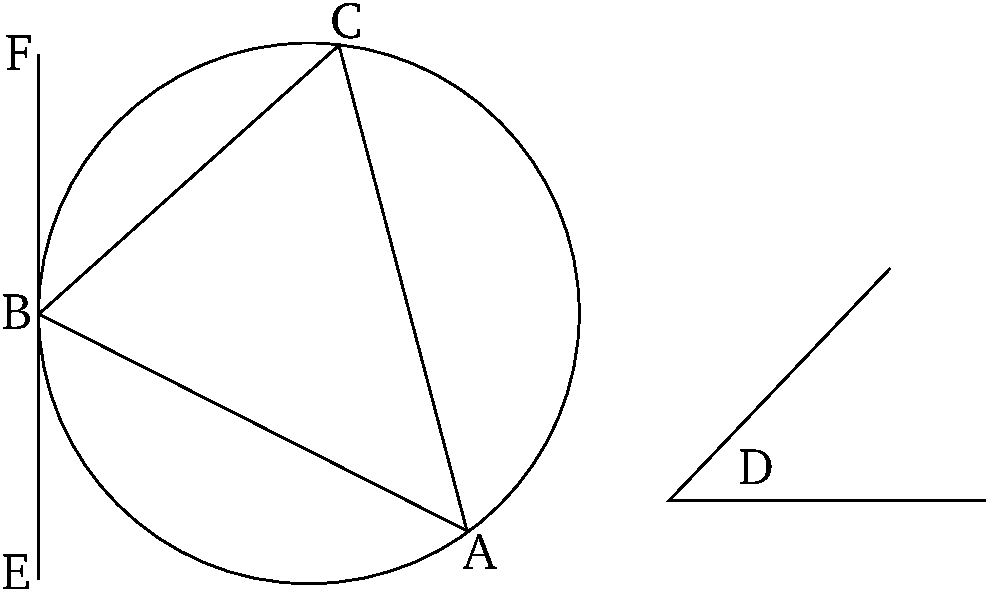
\includegraphics{Book03/fig34e.eps}}

Let $EF$ be drawn touching $ABC$ at point $B$.$^\dag$ And let (angle)
$FBC$, equal to angle $D$, be constructed  on the
straight-line $FB$, at the point $B$ on it [Prop.~1.23].

Therefore, since some straight-line $EF$ touches the circle $ABC$, and
$BC$ has been drawn across (the circle) from the point of contact $B$, angle
$FBC$ is thus equal to the angle constructed in the alternate segment
$BAC$ [Prop.~1.32]. But, $FBC$ is equal to $D$. Thus, the (angle)
in the segment $BAC$ is also equal to [angle] $D$.

Thus, the segment $BAC$, accepting an angle equal to the given
rectilinear angle $D$, has been cut off from the given circle $ABC$. (Which is)
the very thing it was required to do.}
\end{Parallel}
{\footnotesize \noindent$^\dag$ Presumably,
by finding the center of $ABC$ [Prop.~3.1], drawing a straight-line between
the center and point $B$, and then drawing $EF$ through point $B$, at right-angles
to the aforementioned straight-line [Prop.~1.11].}

%%%%%%
% Prop 3.35
%%%%%%
\pdfbookmark[1]{Proposition 3.35}{pdf3.35}
\begin{Parallel}{}{} 
\ParallelLText{
\begin{center}
{\large \ggn{35}.}
\end{center}\vspace*{-7pt}

\gr{Ἐὰν ἐν κύκλῳ δύο εὐθεῖαι τέμνωσιν ἀλλήλαξ, τὸ ὑπὸ τῶν
τῆξ μιᾶξ τμ\kern -.7pt  ημάτων περιεχόμενον ὀρθογώνιον >ίσον ἐστὶ
τῶ| ὑπὸ τῶν τῆξ ἑτέραξ τμ\kern -.7pt  ημάτων περιεθομένῳ ὀρθογωνίῳ.}

\gr{Ἐν γὰρ κύκλῳ τῶ| ΑΒΓΔ δύο εὐθεῖαι αἱ ΑΓ, ΒΔ τεμνέτωσαν ἀλλήλαξ κατὰ τὸ Ε σημεῖον; λέγω, <ότι τὸ ὑπὸ τῶν ΑΕ, ΕΓ
περιεχόμενον ὀρθογώνιον >ίσον ἐστὶ τῶ| ὑπὸ τῶν ΔΕ, ΕΒ
περιεθομένῳ ὀρθογωνίῳ.}

\gr{Εἰ μὲν ο>ῦν αἱ ΑΓ, ΒΔ διὰ τοῦ κέντρου εἰσὶν <ώστε τὸ Ε
κέντρον ε>ῖναι τοῦ ΑΒΓΔ κύκλου, φανερόν, <ότι
>ίσων οὐσῶν τῶν ΑΕ, ΕΓ, ΔΕ, ΕΒ καὶ τὸ ὑπὸ τῶν ΑΕ,
ΕΓ περιεχόμενον ὀρθογώνιον >ίσον ἐστὶ τῶ| ὑπὸ τῶν
ΔΕ, ΕΒ περιεθομένῳ ὀρθογωνίῳ.}

\gr{μ\kern -.7pt  ὴ >έστωσαν δὴ αἱ ΑΓ, ΔΒ διὰ τοῦ κέντρου, καὶ εἰλήφθω τὸ
 κέντρον τοῦ ΑΒΓΔ, καὶ >έστω τὸ Ζ,  καὶ ἀπὸ τοῦ Ζ ἐπὶ
τὰξ ΑΓ, ΔΒ εὐθείαξ κάθετοι >ήθθωσαν αἱ ΖΗ, ΖJ, καὶ ἐπεζεύθθωσαν
αἱ ΖΒ, ΖΓ, ΖΕ.}

\gr{Καὶ ἐπεὶ εὐθεῖά τιξ διὰ τοῦ κέντρου ἡ ΗΖ εὐθεῖάν τινα μ\kern -.7pt  ὴ διὰ
τοῦ κέντρου τὴν ΑΓ πρὸξ ὀρθὰξ τέμνει, καὶ δίθα α\kern -.7pt  ὐτὴν τέμνει;
>ίση >άρα ἡ ΑΗ τῆ| ΗΓ. ἐπεὶ ο>ῦν εὐθεῖα ἡ ΑΓ τέτμ\kern -.5pt  ηται εἰξ μὲν
>ίσα κατὰ τὸ Η, εἰξ δὲ >άνισα κατὰ τὸ Ε, τὸ >άρα ὑπὸ τῶν
ΑΕ, ΕΓ περιεχόμενον ὀρθογώνιον μετὰ τοῦ ἀπὸ τῆξ ΕΗ τετραγώνου
>ίσον ἐστὶ τῶ| ἀπὸ τῆξ ΗΓ; [κοινὸν] προσκείσθω τὸ ἀπὸ τῆξ ΗΖ;
τὸ >άρα ὑπὸ τῶν ΑΕ, ΕΓ μετὰ τῶν ἀπὸ τῶν ΗΕ, ΗΖ >ίσον ἐστὶ
τοῖξ ἀπὸ τῶν ΓΗ, ΗΖ. ἀλλὰ τοῖξ μὲν ἀπὸ τῶν ΕΗ, ΗΖ >ίσον
ἐστὶ τὸ ἀπὸ τῆξ ΖΕ, τοὶξ δὲ ἀπὸ τῶν ΓΗ, ΗΖ >ίσον
ἐστὶ τὸ ἀπὸ τῆξ ΖΓ; τὸ >άρα ὑπὸ τῶν ΑΕ, ΕΓ  μετὰ τοῦ ἀπὸ τῆξ ΖΕ >ίσον  ἐστὶ τῶ| ἀπὸ τῆξ ΖΓ. >ίση δὲ ἡ ΖΓ τῆ| ΖΒ; τὸ
>άρα ὑπὸ τῶν ΑΕ, ΕΓ μετὰ τοῦ ἀπὸ τῆξ ΕΖ >ίσον ἐστὶ
τῶ| ἀπὸ τῆξ ΖΒ. διὰ τὰ α\kern -.3pt  ὐτὰ δὴ καὶ τὸ 
 ὑπὸ  τῶν ΔΕ, ΕΒ μετὰ τοῦ ἀπὸ τῆξ
ΖΕ ἰσον ἐστὶ τῶ| ἀπὸ τῆξ ΖΒ. ἐδείθθη δὲ καὶ τὸ ὑπὸ
τῶν ΑΕ, ΕΓ μετὰ τοῦ ἀπὸ τῆξ ΖΕ >ίσον τῶ| ἀπὸ τῆξ
ΖΒ; τὸ >άρα ὑπὸ τῶν ΑΕ, ΕΓ μετὰ τοῦ ἀπὸ τῆξ ΖΕ >ίσον
ἐστὶ τῶ| ὑπὸ τῶν
ΔΕ, ΕΒ μετὰ τοῦ ἀπὸ τῆξ ΖΕ. κοινὸν ἀφῆ|ρήσθω
τὸ ἀπὸ τῆξ ΖΕ; λοιπὸν >άρα τὸ ὑπὸ
τῶν ΑΕ, ΕΓ περιεχόμενον ὀρθογώνιον >ίσον ἐστὶ τῶ| ὑπὸ
τῶν ΔΕ, ΕΒ περιεθομένῳ ὀρθογωνίῳ.}\\~\\~\\~\\~\\~\\~\\

\epsfysize=1.5in
\centerline{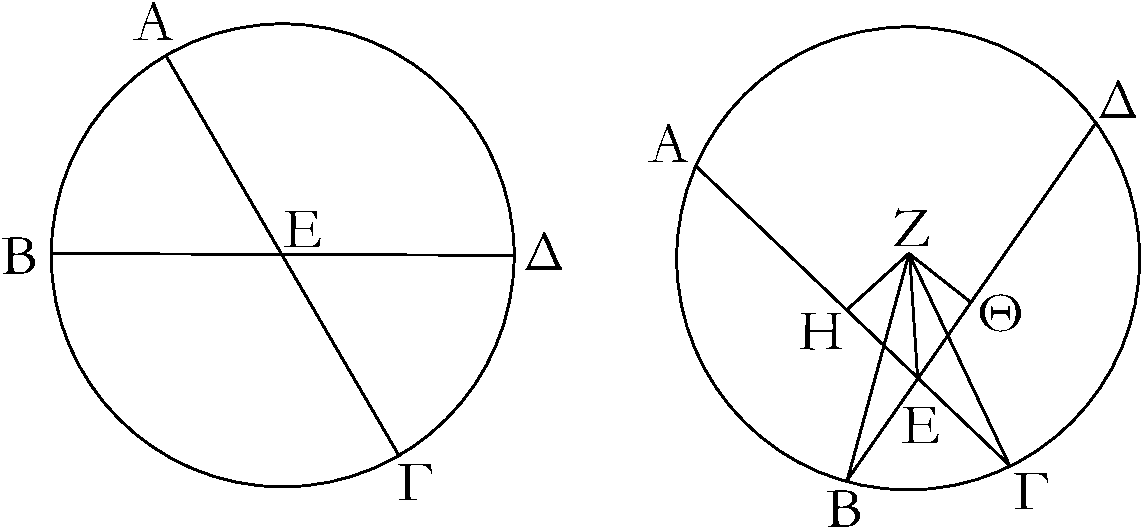
\includegraphics{Book03/fig35g.eps}}

\gr{Ἐὰν >άρα ἐν κύκλῳ εὐθεῖαι δύο τέμνωσιν ἀλλήλαξ, τὸ ὑπὸ τῶν
τῆξ μιᾶξ τμ\kern -.7pt  ημάτων περιεχόμενον ὀρθογώνιον >ίσον ἐστὶ
τῶ| ὑπὸ τῶν τῆξ ἑτέραξ τμ\kern -.7pt  ημάτων περιεθομένῳ ὀρθογωνίῳ;
<όπερ >έδει δεῖχαι.}}

\ParallelRText{
\begin{center}
{\large Proposition 35}
\end{center}

If two straight-lines in a circle cut one another, (then) the rectangle
contained by the pieces of one is equal to the rectangle contained
by the pieces of the other.

For let the two straight-lines $AC$ and $BD$, in the circle $ABCD$,
cut one another at  point $E$. I say that the rectangle contained by
$AE$ and $EC$ is equal to the rectangle contained  by $DE$ and $EB$.

In fact, if $AC$ and $BD$ are through the center (as in the first diagram from the left), so that $E$ is the center
of circle $ABCD$, (then it is) clear that, $AE$, $EC$, $DE$, and $EB$ being equal,
the rectangle contained by $AE$ and $EC$ is also equal to the rectangle
contained by $DE$ and $EB$.

So let $AC$ and $DB$ not be though the center (as in the second diagram from the left), and let the center of $ABCD$ 
be found [Prop.~3.1], and let it be (at) $F$. And let $FG$ and $FH$
be drawn from $F$, perpendicular to the straight-lines $AC$ and $DB$
(respectively) [Prop.~1.12]. And let $FB$, $FC$, and $FE$ 
be joined.

And since some straight-line, $GF$, through the center, cuts at right-angles  some (other) straight-line, $AC$, not through the center,  (then) it also cuts
it in half [Prop.~3.3]. Thus, $AG$ (is) equal to $GC$. Therefore,
since the straight-line $AC$ is cut equally at $G$, and unequally at $E$,
the rectangle contained by $AE$ and $EC$ plus the square on $EG$ is thus
equal to the (square) on $GC$ [Prop.~2.5]. Let the (square) on
$GF$ be added [to both]. Thus, the (rectangle contained) by 
$AE$ and $EC$ plus the (sum of the squares) on $GE$ and $GF$ is equal to
the (sum of the squares) on $CG$ and $GF$. But, the (square) on $FE$ is equal to the (sum of the squares)
on $EG$ and $GF$   [Prop.~1.47],
and the (square)
on $FC$  is equal to the (sum of the squares) on $CG$ and $GF$ [Prop.~1.47]. Thus, the (rectangle contained) by
$AE$ and $EC$ plus the (square) on $FE$ is equal to the (square) on $FC$.
And $FC$ (is) equal to $FB$. Thus, the (rectangle contained) by
$AE$ and $EC$ plus the (square) on $FE$ is equal to the (square) on $FB$.
So, for the same (reasons), the (rectangle contained) by
$DE$ and $EB$ plus the (square) on $FE$ is equal to the (square) on $FB$.
And the (rectangle contained) by
$AE$ and $EC$ plus the (square) on $FE$ was also shown (to be) equal to the (square) on $FB$. Thus,  the (rectangle contained) by
$AE$ and $EC$ plus the (square) on $FE$ is equal to the (rectangle contained) by
$DE$ and $EB$ plus the (square) on $FE$. Let the (square) on $FE$ be
taken from both. Thus, the remaining rectangle contained by $AE$ and
$EC$ is equal to the rectangle contained by $DE$ and $EB$.

\epsfysize=1.5in
\centerline{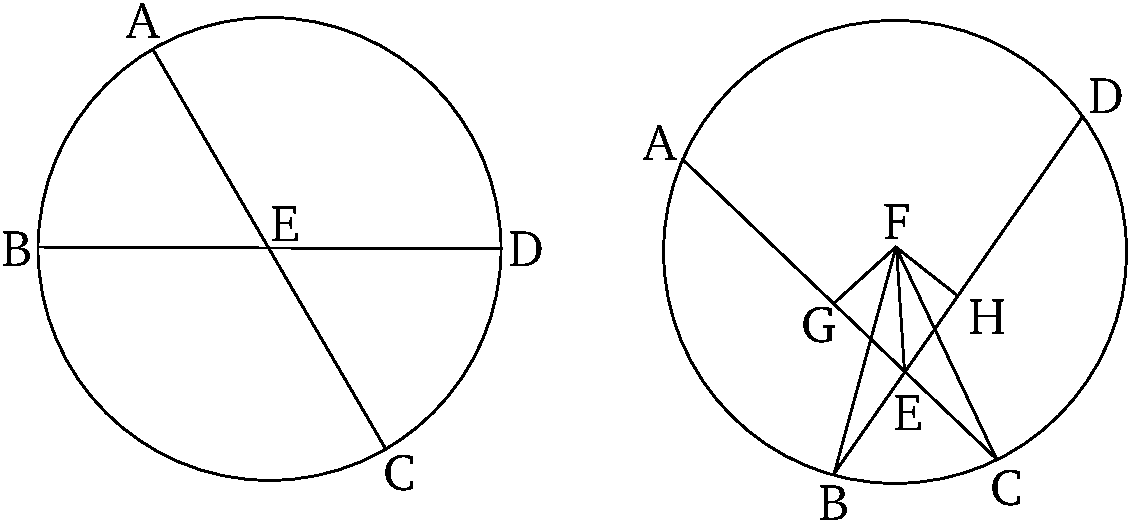
\includegraphics{Book03/fig35e.eps}}

Thus, if two straight-lines in a circle cut one another, (then) the rectangle
contained by the pieces of one is equal to the rectangle contained
by the pieces of the other. (Which is) the very thing it was required to
show.}
\end{Parallel}

%%%%%%
% Prop 3.36
%%%%%%
\pdfbookmark[1]{Proposition 3.36}{pdf3.36}
\begin{Parallel}{}{} 
\ParallelLText{
\begin{center}
{\large \ggn{36}.}
\end{center}\vspace*{-7pt}

\gr{Ἐὰν κύκλου ληφθῆ| τι σημεῖον ἐκτόξ, καὶ ἀπ> α\kern -.7pt  ὐτοῦ πρὸξ τὸν
κύκλον προσπίπτωσι δύο εὐθεῖαι, καὶ ἡ μὲν α\kern -.7pt  ὐτῶν τέμνῃ τὸν
κύκλον, ἡ δὲ ἐφάπτηται, >έσται τὸ ὑπὸ <όληξ τῆξ τεμνούσηξ
καὶ τῆξ ἐκτὸξ ἀπολαμβανομένηξ μεταχὺ τοῦ τε σημείου καὶ
τῆξ κυρτῆξ περιφερείαξ >ίσον τῶ| ἀπὸ τῆξ ἐφαπτομένηξ τετραγώνῳ.}

\gr{Κύκλου γὰρ τοῦ ΑΒΓ εἰλήφθω τι σημεῖον ἐκτὸξ τὸ Δ, καὶ ἀπὸ
τοῦ Δ πρὸξ τὸν ΑΒΓ κύκλον προσπιπτέτωσαν δύο εὐθεῖαι αἱ ΔΓ[Α],
ΔΒ; καὶ ἡ μὲν ΔΓΑ τεμνέτω τὸν ΑΒΓ κύκλον, ἡ δὲ ΒΔ ἐφαπτέσθω;
λέγω, <ότι τὸ ὑπὸ τῶν ΑΔ, ΔΓ περιεχόμενον ὀρθογώνιον
>ίσον ἐστὶ τῶ| ἀπὸ τῆξ ΔΒ τετραγώνῳ.}\\

\epsfysize=1.8in
\centerline{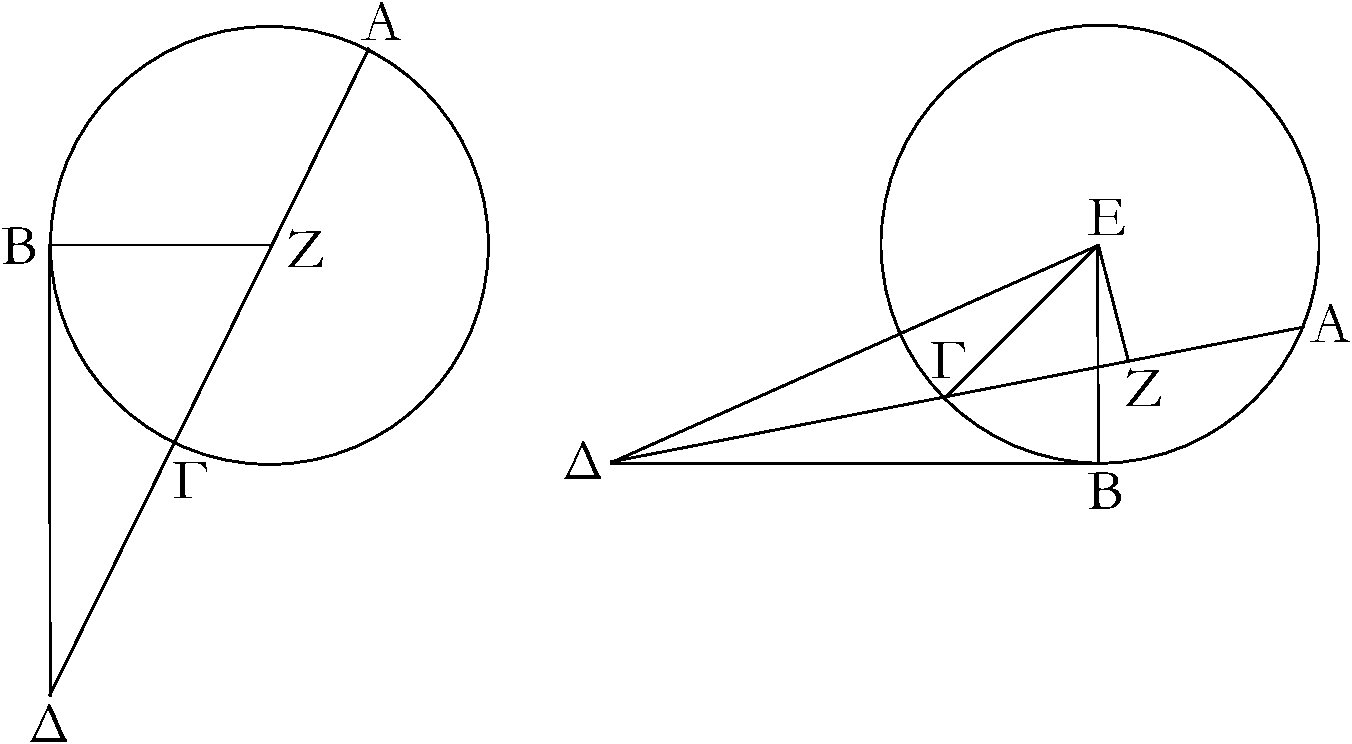
\includegraphics{Book03/fig36g.eps}}

\gr{Ἡ >άρα [Δ]ΓΑ >ήτοι διὰ τοῦ κέντρου ἐστὶν >ὴ ο>ύ. >έστω πρότερον
διὰ τοῦ κέντρου, καὶ >έστω τὸ Ζ κέντρον τοῦ ΑΒΓ κύκλου, καὶ ἐπεζεύθθω ἡ ΖΒ; ὀρθὴ >άρα ἐστὶν ἡ ὑπὸ ΖΒΔ. καὶ ἐπεὶ εὐθεῖα
ἡ ΑΓ δίθα τέτμ\kern -.7pt  ηται κατὰ τὸ Ζ, πρόσκειται δὲ α\kern -.7pt  ὐτῆ| ἡ ΓΔ, τὸ
>άρα ὑπὸ τῶν ΑΔ, ΔΓ μετὰ τοῦ ἀπὸ τῆξ ΖΓ >ίσον
ἐστὶ τῶ| ἀπὸ τῆξ ΖΔ. >ίση δὲ ἡ ΖΓ τῆ| ΖΒ; τὸ >άρα ὑπὸ
τῶν ΑΔ, ΔΓ μετὰ τοῦ ἀπὸ τῆξ ΖΒ >ίσον ἐστὶ τῶ| ἀπὸ τῆξ ΖΔ.
 τῶ| δὲ ἀπὸ τῆξ ΖΔ >ίσα
 ἐστὶ τὰ ἀπὸ τῶν ΖΒ, ΒΔ; τὸ >άρα ὑπὸ τῶν ΑΔ, ΔΓ μετὰ
τοῦ ἀπὸ τῆξ ΖΒ >ίσον ἐστὶ τοῖξ ἀπὸ τῶν ΖΒ, ΒΔ. κοινὸν
ἀφῃρήσθω τὸ ἀπὸ  	τῆξ ΖΒ; λοιπὸν >άρα τὸ ὑπὸ τῶν ΑΔ, ΔΓ
>ίσον ἐστὶ τῶ| ἀπὸ τῆξ ΔΒ ἐφαπτομένηξ.}

\gr{Ἀλλὰ δὴ ἡ ΔΓΑ μ\kern -.7pt  ὴ >έστω διὰ τοῦ κέντρου τοῦ ΑΒΓ κύκλου,
καὶ εἰλήφθω τὸ κέντρον τὸ Ε, καὶ 
ἀπὸ τοῦ Ε ἐπὶ τὴν ΑΓ κάθετοξ >ήθθω ἡ ΕΖ, καὶ ἐπεζεύθθωσαν
αἱ ΕΒ, ΕΓ, ΕΔ; ὀρθὴ >άρα ἐστὶν ἡ ὑπὸ ΕΒΔ. καὶ ἐπεὶ εὐθεῖά
τιξ διὰ τοῦ κέντρου ἡ ΕΖ εὐθεῖάν τινα μ\kern -.7pt  ὴ διὰ τοῦ κέντρου τὴν
ΑΓ πρὸξ ὀρθὰξ τέμνει, καὶ δίθα α\kern -.5pt  ὐτὴν τέμνει; ἡ ΑΖ >άρα τῆ|
ΖΓ ἐστιν >ίση. καὶ ἐπεὶ εὐθεῖα ἡ ΑΓ τέτμ\kern -.3pt  ηται δίθα κατὰ τὸ Ζ
σημεῖον, πρόσκειται δὲ α\kern -.7pt  ὐτῆ| ἡ ΓΔ, τὸ >άρα ὑπὸ τῶν ΑΔ, ΔΓ μετὰ
τοῦ ἀπὸ τῆξ ΖΓ >ίσον ἐστὶ τῶ| ἀπὸ τῆξ ΖΔ. κοινὸν προσκείσθω τὸ
ἀπὸ τῆξ ΖΕ; τὸ >άρα ὑπὸ τῶν ΑΔ, ΔΓ μετὰ τῶν ἀπὸ
τῶν ΓΖ, ΖΕ >ίσον ἐστὶ τοῖξ ἀπὸ τῶν ΖΔ, ΖΕ. τοῖξ δὲ ἀπὸ
τῶν ΓΖ, ΖΕ >ίσον ἐστὶ τὸ ἀπὸ τῆξ ΕΓ; ὀρθὴ γὰρ [ἐστιν]
 ἡ ὑπὸ ΕΖΓ [γωνία]; τοῖξ δὲ ἀπὸ τῶν ΔΖ, ΖΕ >ίσον ἐστὶ
 τὸ ἀπὸ τῆξ ΕΔ; τὸ >άρα ὑπὸ τῶν ΑΔ, ΔΓ μετὰ τοῦ ἀπὸ
 τῆξ ΕΓ >ίσον ἐστὶ τῶ| ἀπὸ τῆξ ΕΔ. >ίση
 δὲ ἡ ΕΓ τὴ| ΕΒ; 
 τὸ >άρα ὑπὸ τῶν ΑΔ, ΔΓ μετὰ τοῦ ἀπὸ τῆξ ΕΒ >ίσον
 ἐστὶ τῶ| >άπὸ τῆξ ΕΔ.
  τῶ| δὲ ἀπὸ τῆξ ΕΔ
 >ίσα ἐστὶ τὰ ἀπὸ τῶν ΕΒ, ΒΔ; ὀρθὴ γὰρ ἡ ὑπὸ ΕΒΔ γωνία;
 τὸ >άρα ὑπὸ τῶν ΑΔ, ΔΓ μετὰ τοῦ ἀπὸ 
τῆξ ΕΒ >ίσον 
 ἐστὶ τοῖξ ἀπὸ τῶν ΕΒ, ΒΔ. κοινὸν ἀφῃρήσθω τὸ ἀπὸ τῆξ
 ΕΒ; λοιπὸν >άρα τὸ ὑπὸ τῶν ΑΔ, ΔΓ >ίσον ἐστὶ τῶ| ἀπὸ τῆξ
 ΔΒ.}
 
 \gr{Ἐὰν >άρα κύκλου ληφθῆ| τι σημεῖον ἐκτόξ, καὶ ἀπ> α\kern -.7pt  ὐτοῦ πρὸξ τὸν
κύκλον προσπίπτωσι δύο εὐθεῖαι, καὶ ἡ μὲν α\kern -.7pt  ὐτῶν τέμνῃ τὸν
κύκλον, ἡ δὲ ἐφάπτηται, >έσται τὸ ὑπὸ <όληξ τῆξ τεμνούσηξ
καὶ τῆξ ἐκτὸξ ἀπολαμβανομένηξ μεταχὺ τοῦ τε σημείου καὶ
τῆξ κυρτῆξ περιφερείαξ >ίσον τῶ| ἀπὸ τῆξ ἐφαπτομένηξ τετραγώνῳ;
<όπερ >έδει δεῖχαι.}}

\ParallelRText{
\begin{center}
{\large Proposition 36}\end{center}

If some point is taken outside a circle, and  two straight-lines
radiate from it towards the circle, and (one) of them cuts the circle, and the (other)
touches (it), (then) the (rectangle contained) by the whole  (straight-line) cutting (the circle), and the (part of it) 
cut off outside (the circle),
between the point and the convex circumference, will be equal to the
square on the tangent (line).

For let some point $D$ be taken outside circle $ABC$, and let two
straight-lines, $DC[A]$ and $DB$, radiate from $D$ towards circle $ABC$. And
let $DCA$ cut circle $ABC$, and let $BD$ touch (it). I say that the rectangle
contained by $AD$ and $DC$ is equal to the square on $DB$.

\epsfysize=1.8in
\centerline{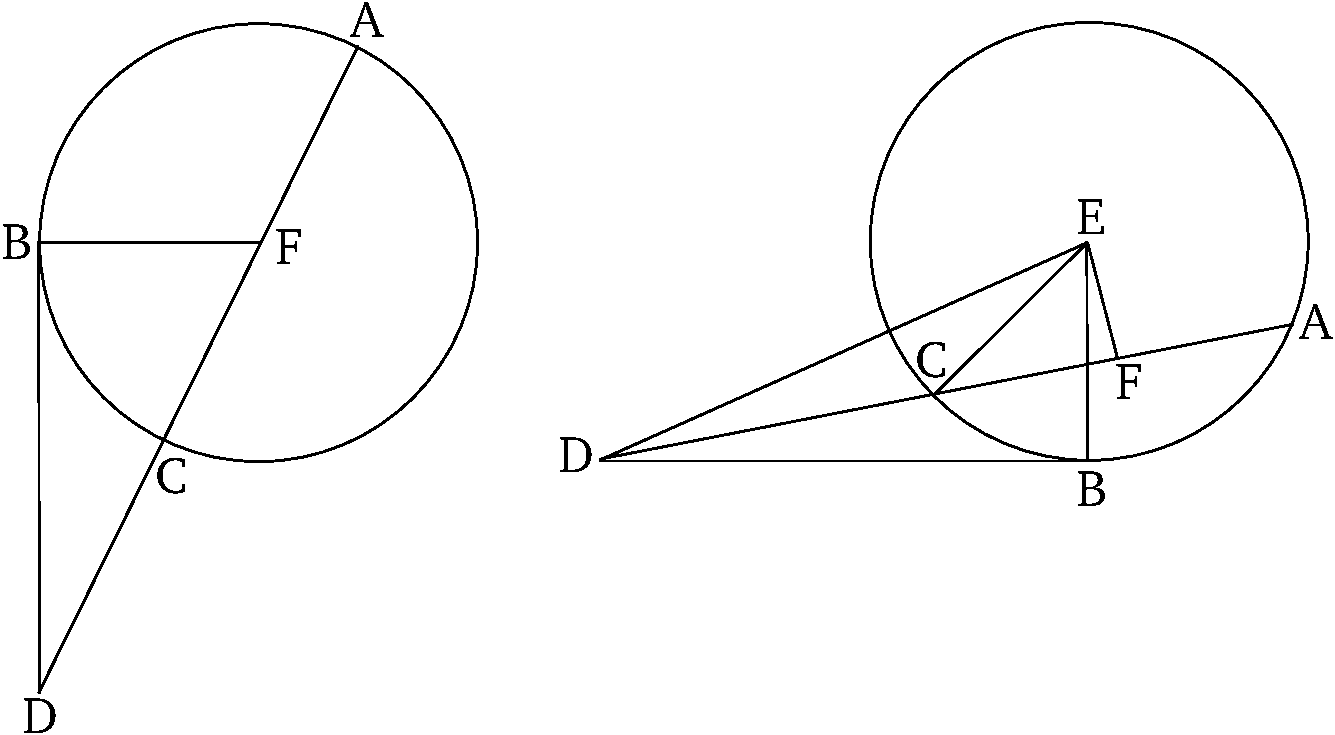
\includegraphics{Book03/fig36e.eps}}

$[D]CA$ is surely either through the center, or not. Let it first of all be
through the center, and let $F$ be the center of circle $ABC$, and let 
$FB$ be joined. Thus, (angle) $FBD$ is a right-angle [Prop.~3.18].
And since straight-line $AC$ is cut in half at $F$, let $CD$ be added to it.
Thus, the (rectangle contained) by $AD$ and $DC$ plus the (square) on $FC$ is
equal to the (square) on $FD$ [Prop.~2.6]. And $FC$ (is) equal to $FB$.
Thus, the (rectangle contained) by $AD$ and $DC$ plus the (square) on $FB$
is equal to the (square) on $FD$. And the (square) on $FD$ is equal to
the (sum of the squares) on $FB$ and $BD$ [Prop.~1.47]. Thus, the
(rectangle contained) by $AD$ and $DC$ plus the (square) on $FB$ is equal
to the (sum of the squares) on $FB$ and $BD$. Let the (square) on $FB$ be subtracted
from both. Thus, the remaining (rectangle contained) by $AD$ and $DC$ 
is equal to the (square) on the tangent $DB$.

And so let $DCA$ not be through the center of circle $ABC$, and let the center $E$
be found, and let $EF$ be drawn from $E$, perpendicular to
$AC$ [Prop.~1.12]. And let $EB$, $EC$, and $ED$ be joined. (Angle)
$EBD$ (is) thus a right-angle [Prop.~3.18]. And since some straight-line, $EF$, through the
center, cuts some (other) straight-line, $AC$, not through the center, at
right-angles, it also cuts it in half [Prop.~3.3]. Thus, $AF$ is equal to
$FC$. And since the straight-line $AC$ is cut in half at point $F$, let $CD$ 
be added to it. Thus, the (rectangle contained) by $AD$ and
 $DC$ plus the
(square) on $FC$ is equal to the (square) on $FD$ [Prop.~2.6]. Let
the (square) on $FE$ be added to both. Thus, the (rectangle contained)
by $AD$ and $DC$ plus the (sum of the squares) on $CF$ and $FE$ is equal to
the (sum of the squares) on $FD$ and $FE$. But  the (square) on $EC$  is equal to the (sum of the squares)
on $CF$ and $FE$. For [angle] $EFC$ [is] a
right-angle [Prop.~1.47]. And the (square) on $ED$ is equal to the (sum of the squares) on $DF$ and
$FE$   [Prop.~1.47]. Thus, the (rectangle
contained) by $AD$ and $DC$ plus the (square) on $EC$ is equal to the (square)
on $ED$. And $EC$ (is) equal to $EB$. Thus, the (rectangle
contained) by $AD$ and $DC$ plus the (square) on $EB$ is equal to the (square)
on $ED$. And the (sum of the squares) on 
$EB$ and $BD$  is equal to  the (square) on $ED$. For $EBD$ (is) a right-angle [Prop.~1.47]. Thus, the (rectangle
contained) by $AD$ and $DC$ plus the (square) on $EB$ is equal to the (sum of the squares)
on $EB$ and $BD$. Let the (square) on $EB$ be subtracted from both. Thus, the remaining
(rectangle contained) by $AD$ and $DC$ is equal to the (square) on $BD$.

Thus, if some point is taken outside a circle, and  two straight-lines
radiate from it towards the circle, and (one) of them cuts the circle, and (the other) touches (it), (then) the (rectangle contained) by the whole  (straight-line) cutting (the circle), and the (part of it) 
cut off outside (the circle),
between the point and the convex circumference, will be equal to the
square on the tangent (line). (Which is) the very thing it was required to show.}
\end{Parallel}

%%%%%%
% Prop 3.37
%%%%%%
\pdfbookmark[1]{Proposition 3.37}{pdf3.37}
\begin{Parallel}{}{} 
\ParallelLText{
\begin{center}
{\large \ggn{37}.}
\end{center}\vspace*{-7pt}

\gr{Ἐὰν κύκλου ληφθῆ| τι σημεῖον ἐκτόξ, ἀπὸ δὲ τοῦ σημείου πρὸξ τὸν
κύκλον προσπίπτωσι δύο εὐθεῖαι, καὶ ἡ μὲν α\kern -.7pt  ὐτῶν τέμνῃ
τὸν κύκλον, ἡ δὲ προσπίπτῃ, >ῆ| δὲ τὸ ὑπὸ [τῆξ] <όληξ τῆξ
τεμνούσηξ καὶ τῆξ ἐκτὸξ ἀπολαμβανομένηξ μεταχὺ τοῦ τε σημείου καὶ
τῆξ κυρτῆξ περιφερείαξ >ίσον τῶ| ἀπὸ τῆξ προσπιπτούσηξ, ἡ
προσπίπτουσα ἐφάψεται τοῦ κύκλου.}

\gr{Κύκλου γὰρ τοῦ ΑΒΓ εἰλήφθω τι σημεῖον ἐκτὸξ τὸ Δ, καὶ ἀπὸ
τοῦ Δ πρὸξ τὸν ΑΒΓ κύκλον προσπιπτέτωσαν δύο εὐθεῖαι αἱ
ΔΓΑ, ΔΒ, καὶ ἡ μὲν ΔΓΑ τεμνέτω τὸν κύκλον, ἡ δὲ ΔΒ προσπιπτέτω,
>έστω δὲ τὸ ὑπὸ τῶν ΑΔ, ΔΓ >ίσον τῶ| ἀπὸ τῆξ ΔΒ. λέγω,
<ότι ἡ ΔΒ ἐφάπτεται τοῦ ΑΒΓ κύκλου.}\\~\\

\epsfysize=1.75in
\centerline{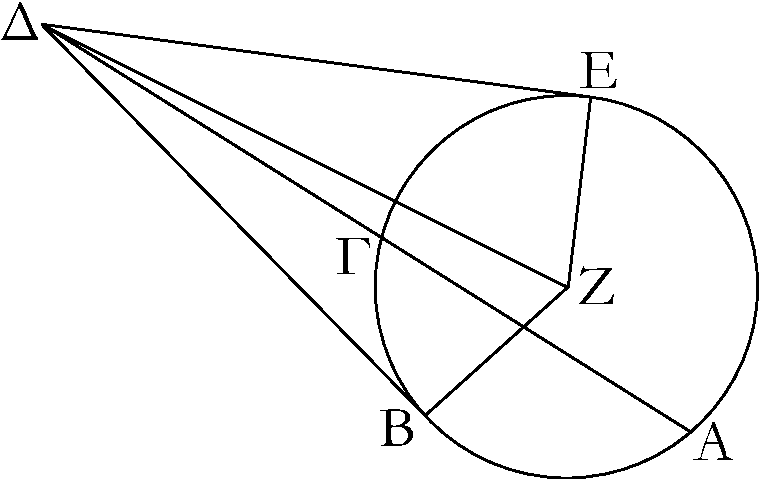
\includegraphics{Book03/fig37g.eps}}

\gr{>'Ηθθω γὰρ τοῦ ΑΒΓ ἐφαπτομένη ἡ ΔΕ, καὶ εἰλήφθω τὸ κέντρον
τοῦ ΑΒΓ κύκλου, καὶ >έστω τὸ Ζ, καὶ ἐπεζεύθθωσαν αἱ ΖΕ, ΖΒ, ΖΔ.
ἡ >άρα ὑπὸ ΖΕΔ ὀρθή ἐστιν. καὶ ἐπεὶ ἡ ΔΕ ἐφάπτεται τοῦ
ΑΒΓ κύκλου, τέμνει δὲ ἡ ΔΓΑ, τὸ >άρα ὑπὸ τῶν ΑΔ, ΔΓ
>ίσον ἐστὶ τῶ| ἀπὸ τῆξ ΔΕ. >ῆν δὲ καὶ τὸ ὑπὸ τῶν
ΑΔ, ΔΓ >ίσον τῶ| ἀπὸ τῆξ ΔΒ; τὸ >άρα ἀπὸ τῆξ ΔΕ >ίσον ἐστὶ τῶ| ἀπὸ
τῆξ ΔΒ;
>ίση >άρα ἡ ΔΕ τῆ| ΔΒ.
ἐστὶ δὲ καὶ ἡ ΖΕ τῆ| ΖΒ >ίση; δύο δὴ αἱ ΔΕ, ΕΖ δύο ταῖξ ΔΒ, ΒΖ
>ίσαι εἰσίν; καὶ βάσιξ α\kern -.7pt  ὐτῶν κοινὴ ἡ ΖΔ; γωνία >άρα ἡ ὑπὸ
ΔΕΖ γωνίᾳ τῆ| ὑπὸ ΔΒΖ ἐστιν >ίση. ὀρθὴ δὲ ἡ ὑπὸ ΔΕΖ; ὀρθὴ
>άρα καὶ ἡ ὑπὸ ΔΒΖ. καί ἐστιν ἡ ΖΒ ἐκβαλλομένη διάμετροξ;
ἡ δὲ τῆ| διαμέτρῳ τοῦ κύκλου πρὸξ ὀρθὰξ ἀπ>
>άκραξ ἀγομένη ἐφάπτεται τοῦ κύκλου; ἡ ΔΒ >άρα ἐφάπτεται
τοῦ ΑΒΓ κύκλου. ὁμοίωξ δὴ δειθθήσεται, κ>ὰν τὸ κέντρον  ἐπὶ
τῆξ ΑΓ τυγθάνῃ.}

\gr{Ἐὰν >άρα κύκλου ληφθῆ| τι σημεῖον ἐκτόξ, ἀπὸ δὲ τοῦ σημείου πρὸξ τὸν
κύκλον προσπίπτωσι δύο εὐθεῖαι, καὶ ἡ μὲν α\kern -.7pt  ὐτῶν τέμνῃ
τὸν κύκλον, ἡ δὲ προσπίπτῃ, >ῆ| δὲ τὸ ὑπὸ  <όληξ τῆξ
τεμνούσηξ καὶ τῆξ ἐκτὸξ ἀπολαμβανομένηξ μεταχὺ τοῦ τε σημείου καὶ
τῆξ κυρτῆξ περιφερείαξ >ίσον τῶ| ἀπὸ τῆξ προσπιπτούσηξ, ἡ
προσπίπτουσα ἐφάψεται τοῦ κύκλου; <όπερ >έδει δεῖχαι.}}

\ParallelRText{
\begin{center}
{\large Proposition 37}
\end{center}

If some point is taken outside a circle, and two straight-lines radiate
from the point towards the circle, and one of them cuts the circle, and the
(other) meets (it), and the (rectangle contained) by the whole (straight-line)
cutting (the circle), and the (part of it) 
cut off outside (the circle),
between the point and the convex circumference,  is equal to the (square)
on the (straight-line) meeting (the circle), (then) the (straight-line)
meeting (the circle) will touch the circle.

For let some point $D$ be taken outside circle $ABC$, and let two
straight-lines, $DCA$ and $DB$, radiate from $D$ towards circle $ABC$, and
let $DCA$ cut the circle, and let $DB$ meet (the circle). And let the (rectangle
contained) by $AD$ and $DC$ be equal to the (square) on $DB$. I say that $DB$ touches circle $ABC$.

\epsfysize=1.75in
\centerline{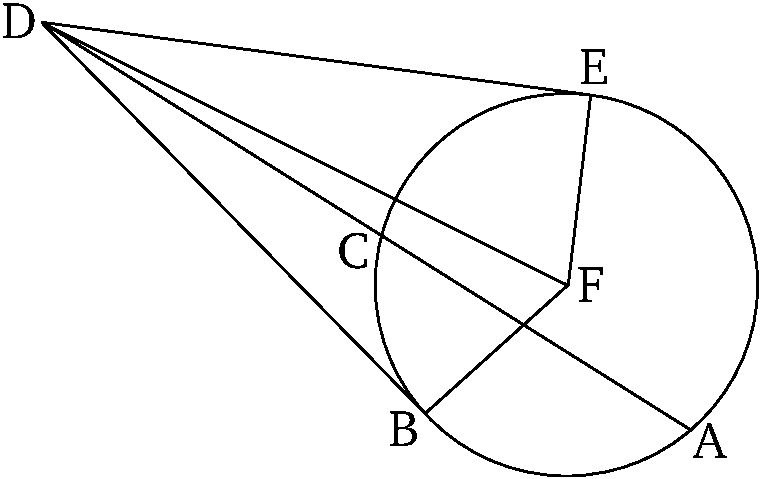
\includegraphics{Book03/fig37e.eps}}

For let $DE$ be drawn touching $ABC$ [Prop. 3.17], and let the center of the circle
$ABC$ be found, and let it be (at) $F$. And let $FE$, $FB$, and $FD$ 
be joined. (Angle) $FED$ is thus a right-angle [Prop.~3.18].
And since $DE$ touches circle $ABC$, and $DCA$ cuts (it), the (rectangle contained) by $AD$ and $DC$ is thus equal to the (square) on $DE$ [Prop.~3.36]. And the (rectangle contained) by $AD$ and $DC$ was also equal
to the (square) on $DB$.  Thus, the (square) on $DE$ is equal to the
(square) on $DB$. Thus, $DE$ (is) equal to $DB$. And $FE$ is also equal to
$FB$. So the two (straight-lines) $DE$, $EF$ are equal to the two (straight-lines)
$DB$, $BF$ (respectively).  And their base, $FD$, is common. Thus, angle $DEF$ is equal to
angle $DBF$ [Prop.~1.8]. And $DEF$ (is) a right-angle. Thus, $DBF$
(is) also a right-angle. And $FB$ produced is a diameter, And a (straight-line)
drawn at right-angles to a diameter of a circle, at its extremity, touches the
circle [Prop.~3.16~corr.]. Thus, $DB$ touches circle $ABC$. 
Similarly, (the same thing) can be shown, even if the center happens to be
on $AC$.

Thus, if some point is taken outside a circle, and two straight-lines radiate
from the point towards the circle, and one of them cuts the circle, and the
(other) meets (it), and the (rectangle contained) by the whole (straight-line)
cutting (the circle), and the (part of it) 
cut off outside (the circle),
between the point and the convex circumference,  is equal to the (square)
on the (straight-line) meeting (the circle), (then) the (straight-line)
meeting (the circle) will touch the circle. (Which is) the very thing it was
required to show.}
\end{Parallel}

\newpage~\thispagestyle{empty}
